% Document template based on LNCS, adapted by Matt Welsh <mdw@cs.berkeley.edu>

% This version is adapted to use PDFTEX to render to PDF directly. 
% If you want to use dvi, you need to change any figures to use '.eps'
% rather than '.pdf', and probably get rid of the hyperref package.

\documentclass[10pt]{article}
\usepackage{program}
\usepackage{acm-style10} % ACM proceedings formatting
\usepackage{times}  % Use Adobe Times font set
\usepackage{epsfig,twocolumn}
\usepackage{url}
\usepackage{textcomp}
\usepackage{usenix}
\usepackage[english]{babel} % mdw: Required to get good hyphenation on RH6.0
                            % (fixed in RH6.1)
\usepackage{graphicx} 
\usepackage{color}

% This will generate links within the PDF as well as a set of bookmarks
% \usepackage[colorlinks,pdfpagemode=None]{hyperref} 

%\def\dsp{\def\baselinestretch{0.92}\large\normalsize}
%\def\dsp{\def\baselinestretch{0.92}}
%\dsp
%\def\dsp{\def\baselinestretch{1.0}}
%\dsp

% DO NOT REMOVE THIS DEFINITION --- IF I HAVE LEFT AN XXXNOTE IN THE
% TEXT IT NEEDS TO BE ADDRESSED AND NOT HIDDEN!
\newcommand{\XXXnote}[1]{{\bf\color{red} XXX: #1}}
%\newcommand{\XXXnote}[1]{}

%\pagestyle{plain}
\pagestyle{empty}
%\pagenumbering{arabic}

%set dimensions of columns, gap between columns, and space between
%paragraphs
%\setlength{\textheight}{9.25in}
\setlength{\textheight}{9.0in}
\setlength{\columnsep}{0.25in}
\setlength{\textwidth}{6.75in}
\setlength{\footskip}{0.0in}
%\setlength{\topmargin}{-0.25in}
\setlength{\topmargin}{0.0in}
\setlength{\headheight}{0.0in}
\setlength{\headsep}{0.0in}
%\setlength{\oddsidemargin}{-0.15in}
\setlength{\oddsidemargin}{-0.125in}
\setlength{\evensidemargin}{0in}
\setlength{\parindent}{1pc}
\setlength{\itemindent}{0.0in}
%\setlength{\parskip}{\baselineskip}
\setlength{\baselineskip}{12pt}

%\setlength{\textheight}{9.25in}
%\setlength{\columnsep}{0.33in}
%\setlength{\textwidth}{7.4in}
%\setlength{\footskip}{0.0in}
%\setlength{\topmargin}{-0.25in}
%\setlength{\headheight}{0.0in}
%\setlength{\headsep}{0.0in}
%\setlength{\oddsidemargin}{-.45in}
%%\setlength{\oddsidemargin}{0in}
%\setlength{\parindent}{1pc}
%%\setlength{\parskip}{\baselineskip}

\begin{document}
% MDW: This needs to be HERE (after the \begin{document})
%\setlength{\baselineskip}{12pt}

%don't want date printed
\date{}

%%%%%%%%%%%% THIS IS WHERE WE PUT IN THE TITLE AND AUTHORS %%%%%%%%%%%%

\title{{\ttlfnt Fidelity and Yield in a \\ Volcano Monitoring Sensor
Network}}
\author{{\aufnt Geoff Werner-Allen$^\star$, Konrad Lorincz$^\star$, 
Jeff Johnson$^\dag$, Jonathan Lees$^\ddag$, and Matt Welsh$^\star$} \\
{\affaddr $^\star$ Division of Engineering and Applied Sciences, Harvard University} \\
{\affaddr $^\dag$ Dept. of Earth Sciences, University of New Hampshire} \\
{\affaddr $^\ddag$ Dept. of Geological Sciences, University of North
Carolina}}
\maketitle
%\copyrightspace

\thispagestyle{empty}

%%%%%%%%%%%%%  ABSTRACT GOES HERE %%%%%%%%%%%%%%

\subsection*{Abstract}
%\abstract{
\begin{small}
%\setlength{\baselineskip}{20pt}
We present a science-centric evaluation of a 19-day sensor
network deployment at Reventador, an active volcano in Ecuador.
Each of the 16~sensors continuously sampled seismic and acoustic 
data at 100~Hz. Nodes used an event-detection algorithm to trigger 
on interesting volcanic activity and initiate reliable data transfer 
to the base station. During the deployment, the network recorded
229~earthquakes, eruptions, and other seismoacoustic events. 
\end{small}

%\setlength{\baselineskip}{9pt}
\begin{small}
The science requirements of reliable data
collection, accurate event detection, and high timing precision 
drive sensor networks in new directions for geophysical monitoring.
The main contribution of this paper is an evaluation of the sensor
network as a scientific instrument, holding it to the standards
of existing instrumentation in terms of data {\em fidelity} (the
quality and accuracy of the recorded signals) and {\em yield} (the quantity
of the captured data).  
We describe an approach to {\em time rectification} of the acquired 
signals that can recover accurate timing despite failures of the 
underlying time synchronization protocol. In addition, we perform a 
detailed study of the sensor network's data using a direct comparison 
to a standalone data logger, as well as an investigation of seismic 
and acoustic wave arrival times across the network. 
%\setlength{\baselineskip}{9pt}
\end{small}
%}

%%%%%%%%%%%%%  BODY OF PAPER GOES HERE %%%%%%%%%%%%%%

\tensize
\setlength{\baselineskip}{12pt}

%\setlength{\baselineskip}{11.5pt}
\chapter{Introduction}
\label{chap-intro}

An emerging application for wireless sensor networks is their use in medical
care. Many medical applications place new demands on sensor network designs.
They often involve variable data rates, multiple receivers, and mobile
nodes. Most existing sensor network designs do not adequately support these
requirements, focusing instead on aggregating small amounts of data from nodes
at fixed locations. Therefore a gap exists between existing sensor network
architectures and the requirements of medical applications.

In this dissertation, we bridge the gap by making three contributions: we
propose CodeBlue medical sensor network architecture, TinyADMR ad-hoc multicast routing protocol, and LiveNet passive monitoring infrastructure.
With CodeBlue, we address the challenges of providing a flexible 
and implementable system architecture for mote-based medical
sensor networks. TinyADMR addresses challenges in multicast routing with the
existence of low quality radio links, memory and bandwidth limitations.
LiveNet addresses the challenges for evaluating deployed medical sensor
networks by reconstructing network dynamics without introducing additional
overhead to the network. We evaluate CodeBlue, TinyADMR and LiveNet
with an indoor sensor network testbed and with a disaster drill deployment.

\section{Medical sensor networks}

The convergence of several new hardware technologies, including MEMS, low
power processors, and low power radio, has enabled a new class of computing
platform: wireless sensors. Wireless sensors combine the capability of
sensing, computation, and wireless communication into a single physical
package, enabling a wide range of applications. Over the past decade, sensor
networks research community has explored the use of wireless sensors in
military target tracking and environmental monitoring such as habitats,
forests, volcanoes, civil infrastructures, factory equipments, and home energy
usage.

One common characteristic of most conventional sensor networks is that they
are intended for deployments of stationary nodes that transmit data at
relatively low rates, with a focus on best-effort data collection at a central
base station. Although the sensor networks research community has made
tremendous progress in perfecting networking and operating system support in
this space, we argue that there is a lack of adequate architectural
support for one emerging and important application domain: medical care.

In a hospital or clinic, outfitting every patient with tiny,
wearable wireless vital sign sensors allows doctors, nurses and other
caregivers to continuously monitor the status of their patients.  In
an emergency or disaster scenario, the same technology would enable
medics to more effectively care for large numbers of casualties.
First responders could receive immediate notifications on any changes
in patient status, such as respiratory failure or cardiac arrest.
Wireless sensors can augment or replace existing wired telemetry
systems for many specific clinical applications, such as physical
rehabilitation or long-term ambulatory monitoring.

A typical scenario involves many patients wearing sensors that monitor basic
vital signs such as heart rate or blood oxygen saturation. A small number of
medical personnel are responsible for continuously monitoring the patients
using devices such as laptops or PDAs. Using the real-time information
retrieved from the network, the medical team can treat
patients who need urgent care more efficiently.


\subsection{Application requirements}

Medical sensor networks have several different characteristics than
conventional sensor network applications. The sensors are worn by patients and the
data sinks are mobile computers carried by doctors or nurses so that the nodes
in the network are not stationary. Unlike typical sensor networks, there are
likely to be more than one data sinks in the network. Nodes can also join or
leave the network dynamically. Furthermore, the data traffic pattern is
on-demand and dynamic. Different doctors may be interested in real-time status
of different groups of patients and the groups can potentially overlap. There may
also be interests for different types or resolutions of sensor data.
Conventional sensor network architectures are inadequate in such scenarios
because the system cannot assume fixed sensor queries, sampling rate and
static traffic pattern. 


%% data may have different priorities associated with it

\subsection{Resource limitation}

In addition to meeting a different set of application requirements, medical sensor
networks, as conventional sensor network systems, face the challenges from
severe
resource limitations of the low power sensor platforms. To be practical, the
sensor nodes must be light-weight, low power and low cost so that they can be
wearable, have long enough battery lifetime and be affordable. This entails
the use of low power radio and low power processor.  For example, the mote
platform, MicaZ~\cite{micaz}, that we use for our medical sensor networks has
4~KB of RAM, a 4~MHz 8-bit CPU and a low power IEEE 802.15.4 radio with
maximum transmit power at 0 dBm. The implication of such a limited platform is
that the software running on the mote cannot be overly computationally
intensive or require large amount of memory. Yet, the system must be responsive enough
to handle complex
interactions with the environment such as sampling medical sensors and
performing radio communication in time. As a result, we not only have to find
a new architecture that fulfills the application requirements, it must also be
designed carefully so that it is light weight enough to fit into the platform
but complex enough to fulfill the application demands. 

\section{Systems challenges for medical sensor networks}

We outline a set of challenges identified through the process of designing,
implementing, deploying, and evaluating a medical sensor network. First of
all, there needs to be a new network architecture to efficiently support the
type of queries and traffic patterns for medical sensor networks. Secondly,
to support the new architecture, it is necessary to provide multicast routing
capability on resource-limited sensor nodes. Third, studying a deployed
medical sensor network requires a non-trivial network monitoring infrastructure.

\subsection{A new network architecture}

In contrast to conventional sensor network applications, medical monitoring
must support a large number of patient sensors deployed in a hospital or
disaster site, a variety of data rates, and multiple mobile receiving
devices, such as PDAs carried by doctors or medics. Moreover, medical
monitoring cannot make use of traditional
in-network aggregation since it is not generally meaningful to combine data
from multiple patients. The goal is instead to efficiently deliver information
to the correct receivers. Therefore, there is a significant gap between
existing sensor network designs and the requirements of medical monitoring. 

Supporting such broad range of requirements demands a new approach to
sensor network design. To bridge the technology gap, we propose CodeBlue, an
architecture for medical sensor networks that provides a set of protocols and
services tailored for this application domain. CodeBlue includes
a publish/subscribe communication model, a rich query interface for periodic
and triggered collection of sensor data, a dynamic sensor discovery protocol,
and a programmatic external interface based on Web Services standards.
CodeBlue provides a high-level interface to the network, making it easy to
support new sensor types and applications that tie into real-time medical
sensor data.

\subsection{Multicast on resource limited sensor nodes}

By reviewing the application requirements of medical sensor networks, it
becomes clear that an ad-hoc multicast routing protocol is more adequate
than the conventional many-to-one data collection tree routing approach.
Fortunately there are existing multicast protocols designed for ad-hoc mobile
networks. However, after the attempt to implement one such protocol, ADMR, on
our resource limited sensor platform, we have discovered several challenges
that were not foreseen by the original designers. In order to achieve
acceptable packet delivery ratio, we have to use different routing metrics that
involves the use of link quality information. We have also
investigated the challenges to scale the network within the memory and
bandwidth limitations on the sensor platform.

\subsection{Deployment support}

To find out whether a design is practical for realistic use, one needs to
deploy the network and evaluate the performance in a realistic environment.
For this purpose, we have conducted a deployment study of the CodeBlue
network. It is necessary to record system behavior in order to study
the correctness and performance of the network during the deployment. Under severe
resource constraints on CPU, memory and bandwidth, it is not practical to
record such information on the sensor nodes locally or transmit the logged
information over the radio. To overcome this problem, we have designed and
built LiveNet, an entirely passive monitoring infrastructure for
reconstructing dynamics of deployed sensor networks.  LiveNet is passive and
therefore does not require changing the application code or incur any
additional resource consumption in the network. Yet, it is able provide
valuable information for evaluating and debugging the deployed network.

\section{Dissertation outline}

The remainder of the dissertation is organized as follows.

Chapter 2 considers background and related work. This chapter introduces 
existing work in sensor networks and ad-hoc networking research community that 
are related to medical sensor networks. We also provide an overview of target
hardware platforms of this thesis.

Chapter 3 presents the requirements for a large class of medical sensor
network applications and a new software architecture to meet these
needs. We first propose the CodeBlue network architecture by presenting the
system goals and overall architecture design. We then describe individual
components
to discuss the design trade-offs in detail. Our key contributions include
proposing publish/subscribe as the appropriate networking abstraction for
a medical sensor network and designing CodeBlue Query (CBQ) interface, which
provides a programmatic interface to the medical sensor network.

Chapter 4 presents our approach to achieving efficient publish/subscribe
communication in sensor networks with mobile nodes, based on the
ADMR~\cite{admr-mobihoc01} {\em ad-hoc\/} multicast routing
protocol. We first describe the challenges encountered when designing and 
implementing the multicast layer to support publish/subscribe communication 
model for CodeBlue. We identify the
challenges from unreliable wireless radio links, memory constraints and
bandwidth constraints. We also explore and evaluate different route discovery
and expiration strategies. The key contributions include two new 
routing metrics that exploit link quality information and identifying
scalability limitations from memory and bandwidth constraints.

Chapter 5 describes LiveNet passive monitoring infrastructure. This chapter 
covers the architecture of LiveNet that involves passive sniffers, trace
merging algorithm and a set of analyses that are used to analyze CodeBlue
deployments. We also present the results of an extensive validation study of 
LiveNet's performance and accuracy with a set of controlled experiments with 
an indoor testbed, MoteLab.

Chapter 6 covers implementation and detailed performance evaluation of
CodeBlue network architecture.  We present evaluation of CodeBlue both on a
sensor network testbed and with a disaster drill deployment.  The testbed
experiments evaluate CodeBlue in scalability, fairness, latency, jitter and
effect of mobility. Then we present a deployment study that was part of a disaster
drill simulating a bus accident. Using data from LiveNet, we are able to
analyze the traffic load, network hotspots, routing paths, and query yield for
this deployment.

Chapter 7 contains lessons learned from the experience of 
designing, implementing, deploying and evaluating medical sensor networks and
provide potential future research directions. 

Chapter 8 concludes.
 
\section{Background}
\label{evaluation-sec-background}


%\subsection{Previous work}

% Tungurahua and Reventador deployment
%Our group is one of the first to explore the use of low-power 
%wireless sensor networks for geophysical monitoring, particularly 
%on active volcanoes. Although wireless telemetry is used on 
%seismic arrays at dozens of volcanoes worldwide, such installations involve 
%large, power-hungry equipment that is not well-suited for rapid, 
%dense deployments. As a result, even many of the most most threatening 
%and active volcanoes (e.g., Mount St. Helens~\cite{malone-81}) maintain 
%networks of less than ten stations.
%One of the primary limitations of volcano seismological studies is simply
%the lack of spatial coverage on a particular volcano.  
%This is true of
%heavily-monitored volcanoes like Mt. St. Helens and Mt. Fuji as well as
%on remote locations in Ecuador.

%Our team has been collaborating for the last two years and has deployed
%two wireless arrays on volcanoes in Ecuador. Our first deployment in
%July 2004 at Volc\'{a}n Tungurahua demonstrated the proof-of-concept, 
%involving three wireless sensor nodes sampling continuous infrasonic 
%time series data~\cite{volcano-agu04,volcano-ewsn05}.  
%The sensor array transmitted continuous, real-time infrasonic signals to
%a base-station laptop via a radio modem 9~km from the deployment site.
%The network operated for 54~hours and collected data on a dozen
%eruptive events during this time. This deployment helped us to optimize
%node placement, packaging, and radio communication in a challenging
%environment. The second installation at Volc\'{a}n Reventador is the
%subject of this paper and is described in the next section.

%In this paper we focus on our second deployment in August 2005, 
%in which we deployed a larger, more sophisticated network on the 
%upper flanks of Volc\'{a}n Reventador. A previous magazine 
%article~\cite{volcano-ieeeic06} detailed the network architecture
%and an overview of the deployment itself. Briefly, the network 
%consisted of 16~nodes, each with seismometers and microphones, 
%distributed over a 3~km extent running radially from the vent. 


\section{System Architecture}
\label{evaluation-sec-design}

% 17 Apr 2006 : GWA : Brief overview of system design.  For now I'm going to
%               defer as many details as possible to the evalution sections
%               since we've covered this in some detail in the IEEE article.
%               Also trying to avoid recycling the wording.  I'm working from
%               the paper copy so the skeleton might be similar though.

In this section we provide a brief overview of the design of our volcano
monitoring sensor network and details of the deployment at Reventador. In an
earlier magazine article~\cite{volcano-ieeeic06} we describe the system and
deployment in more detail, although we have not previously published results
evaluating its performance.

\subsection{Sensor hardware}
\label{evaluation-sec-hardware}

\begin{figure}[t]
\label{evaluation-fig-station}
\begin{center}
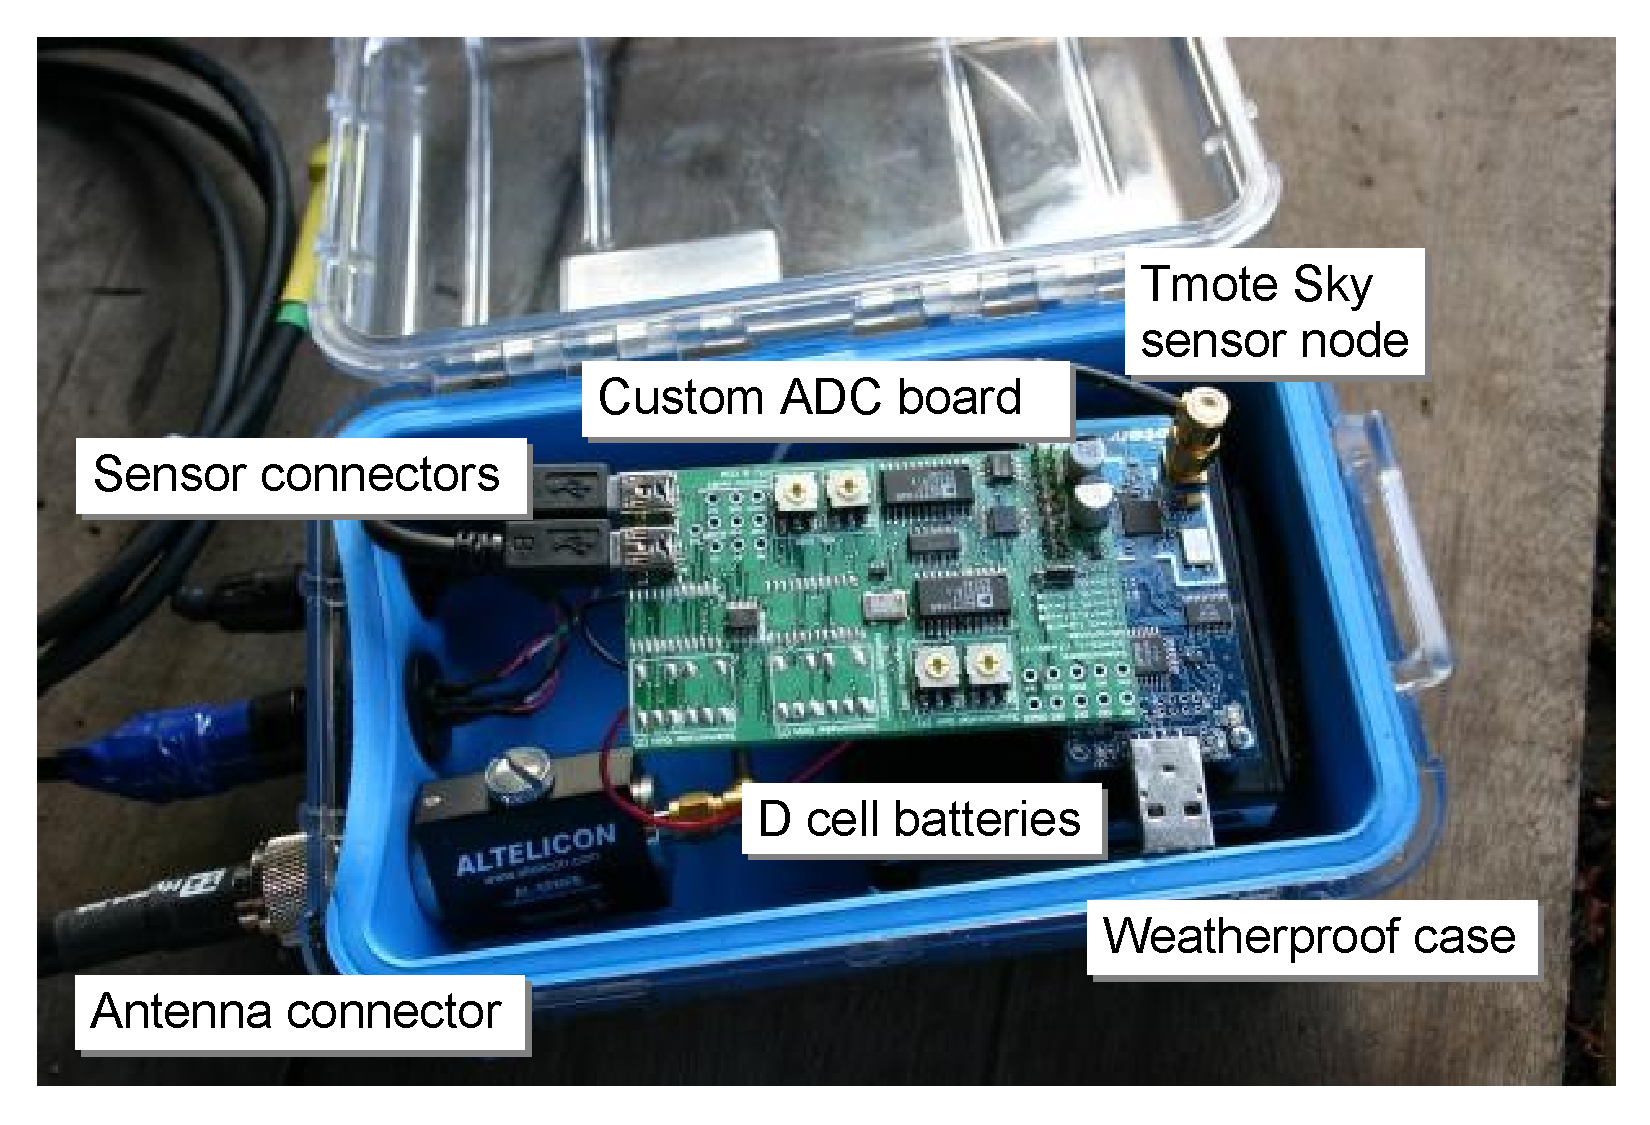
\includegraphics[width=1.0\hsize]{./5-evaluation/figs/pics/Station2-small.pdf}
\end{center}
\caption{\textbf{Our wireless volcano monitoring sensor node.}}
\end{figure}

%We deployed 16 wireless monitoring stations onto Volc\'{a}n Reventador.
%Nodes were arranged in a roughly-linear configuration radiating from the vent
%and spanning over 3km.  Figure REFERENCE shows the locations of each node as
%well as those of several wired monitoring stations deployed nearby.
%\GWAnote{Do we event want to include this figure again? It takes up a lot of
%space but it probably would be nice to have...}

Our wireless sensor node (Figure~\ref{evaluation-fig-station}) is based on
the TMote Sky~\cite{moteiv} platform, which integrates a TI~MSP430 processor,
10~KB of SRAM, 48~KB of program ROM, 1~MByte of flash memory, and a Chipcon
CC2420 radio. All software is implemented in TinyOS~\cite{tinyos-asplos00}.
We designed a custom sampling board that provides four channels of 24-bit
analog-to-digital conversion (TI~AD7710). 
%While the MSP430 provides several channels of ADC, its resolution of 16~bits
%was inadequate for our needs.

Nodes were interfaced to either a single-axis seismometer (GeoSpace GS-11) or
three seismometers in a triaxial configuration (GeoSpace GS-1). 
%The GS-11 sensors are inexpensive and lightweight, but are only sensitive at
%frequencies above 4.5~Hz. In contrast, the GS-1 sensors have a corner
%frequency of 1~Hz but are significantly more expensive and heavy. 
Both sensors are passive instruments; ground motion generates a voltage which
is amplified and digitized by the sampling board.  In addition, each node was
attached to an omnidirectional microphone (Panasonic WM-034BY). This
microphone has been used in other infrasonic monitoring
studies~\cite{johnson-etal-04b}.

% MDW: Node 204 talked to 206 which was 1055 meters away!
Each node was equipped with an 8.5~dBi omnidirectional antenna mounted on
1.5~m of PVC pipe.  This permitted line-of-sight radio range of over 1~km
without amplification; nodes were typically placed 200-400~m apart in our
deployment. Nodes were powered by two D-cell batteries with a lifetime of
approximately 1~week.  Each node was enclosed in a weatherproof Pelican case.

Several other pieces of hardware complete the system. FreeWave radio modems
provided a long-distance radio link between the sensor array and the volcano
observatory, 4.6~km away. A laptop located at the observatory logged data and
was used to monitor and control the network.  Finally, to establish a global
timebase, we used a single Crossbow MicaZ~\cite{xbow} mote interfaced to a
GPS receiver (Garmin OEM~18~LVC).  The GPS receiver provided a 1~Hz pulse
that is accurate to GPS time within 1~$\mu$s, and acted as the root of the
network time synchronization protocol as described in
Section~\ref{evaluation-sec-timing}.

\subsection{Network topology and status monitoring}

Nodes form a multihop routing tree rooted at the gateway node that is
physically attached to the FreeWave modem; we use a variant of
MintRoute~\cite{awoo-multihop} that uses the CC2420's Link Quality Indicator
metric to select routing paths. Each node transmits a {\em status message}
every 10~sec that includes its position in the routing tree, buffer status,
local and global timestamps, battery voltage, and other information. 
%These status messages form the basis of much of the analysis in this paper.
In addition, the base station can issue a {\em command} to each node,
instructing it to respond with an immediate status message, start or stop
data sampling, and set various software parameters.  Commands are propagated
using a simple flooding protocol.  The {\em Deluge} protocol~\cite{deluge}
was also used to permit over-the-air reprogramming and rebooting of nodes.

\subsection{Event detection and data collection}

Because of the high data rates involved (600-1200~bytes/sec from each node)
it is infeasible to continuously transmit all sensor data. Rather, nodes are
programmed to locally detect interesting seismic events and transmit event
reports to the base station. If enough nodes trigger in a short time
interval, the base station attempts to download the last 60~sec of data from
each node.  This design forgoes continuous data collection for increased
resolution following significant seismic events, which include earthquakes,
eruptions, or long-period (LP) events, such as tremor.  The download window
of 60~sec was chosen to capture the bulk of the eruptive and earthquake
events, although many LP events can exceed this window (sometimes lasting
minutes or hours).  To validate our network against existing scientific
instrumentation, our network was designed for high-resolution signal
collection rather than extensive in-network processing.
%In the future we would like to explore more advanced in-network signal
%processing.

During normal operation, each node continuously samples its seismic and
acoustic sensors at 100~Hz, storing the data to flash memory. Data is stored
as 256-byte {\em blocks} in the flash.
%with each block identified by a monotonically increasing {\em block ID}.
Each block 
%is tagged with its ID 
is tagged with the {\em local timestamp} corresponding to the first sample in
the block.  This timestamp is later mapped onto a global time reference as
described in Section~\ref{evaluation-sec-timing}. The 1~Mbyte flash is
treated as a circular buffer storing approximately 20~min of data. 

In addition, nodes run an {\em event detection algorithm} that computes two
exponentially-weighted moving averages (EWMA) over the input signal with
different gain settings. When the ratio between the two EWMAs exceeds a
threshold, the node transmits an event report to the base station.
%$\alpha_{\mathit{high}} > \alpha_{\mathit{low}}$.  That is, the high-gain
%EWMA is more sensitive to changes in the input signal than the low-gain
%EWMA. If the ratio of the high-gain EWMA to the low-gain EWMA exceeds a
%threshold $T$, the node considers the signal to contain a significant event
%and transmits a {\em trigger} message to the base station.
If the base station receives triggers from 30\% of the active nodes within a
10~sec window, it considers the event to be well-correlated and initiates
data collection.

Our reliable bulk-transfer protocol, called {\em Fetch}, operates as follows.
The base station waits for 30~sec following an event before iterating through
all nodes in the network. The base sends each node a command to temporarily
stop sampling, ensuring the event will not be overwritten by subsequent
samples.  For each of the 206~blocks in the 60~sec window, the base sends a
{\em block request} to the node.  The node reads the requested block from
flash and transmits the data as a series of 8~packets.  After a short timeout
the base will issue a repair request to fill in any missing packets from the
block.
%The repair process continues until all packets have been received or a
%timeout occurs. 
Once all blocks have been received or a timeout occurs, the base station
sends the node a command to resume sampling and proceeds to download data
from the next node. 
%The data is logged by the base station laptop for later analysis.

\subsection{Deployment on Volc\'{a}n Reventador}

\begin{figure}[t]
\label{evaluation-fig-schematic}
\begin{center}
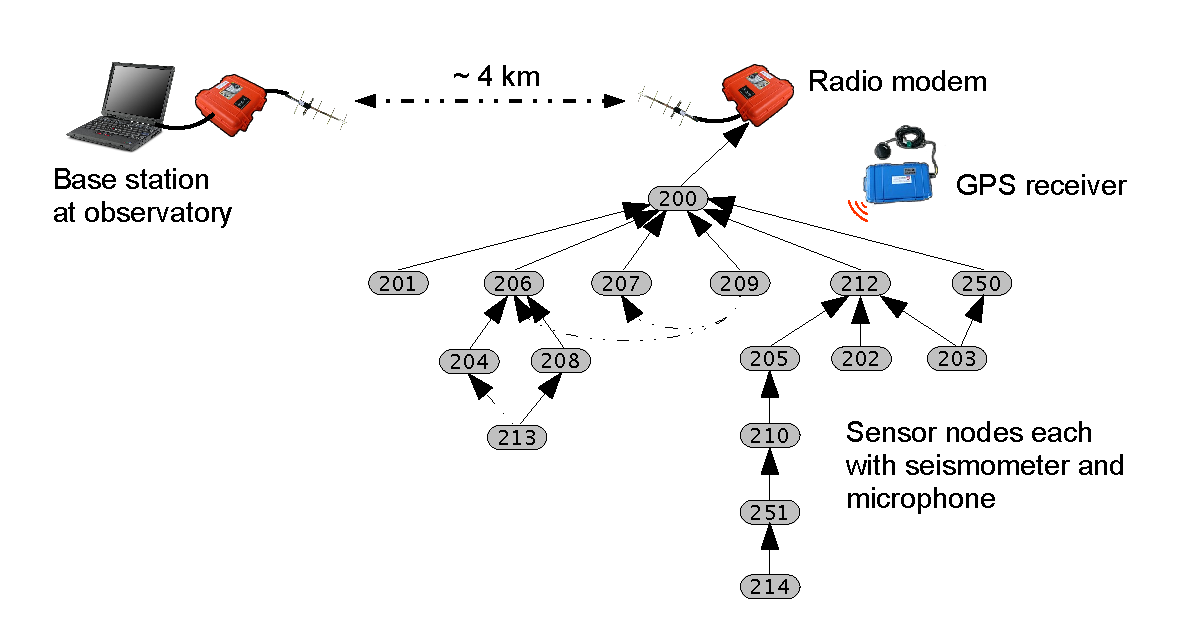
\includegraphics[width=1.0\hsize]{./5-evaluation/figs/pics/schematic2.pdf}
\end{center}
\caption{\textbf{Sensor network architecture.} Nodes form a
multihop routing topology, relaying data via a long-distance radio
modem to the observatory. A GPS receiver is used to establish a global
timebase. The network topology shown here was used during
our deployment at Reventador.}
\end{figure}

\begin{figure}[t]
\label{evaluation-fig-map}
\begin{center}
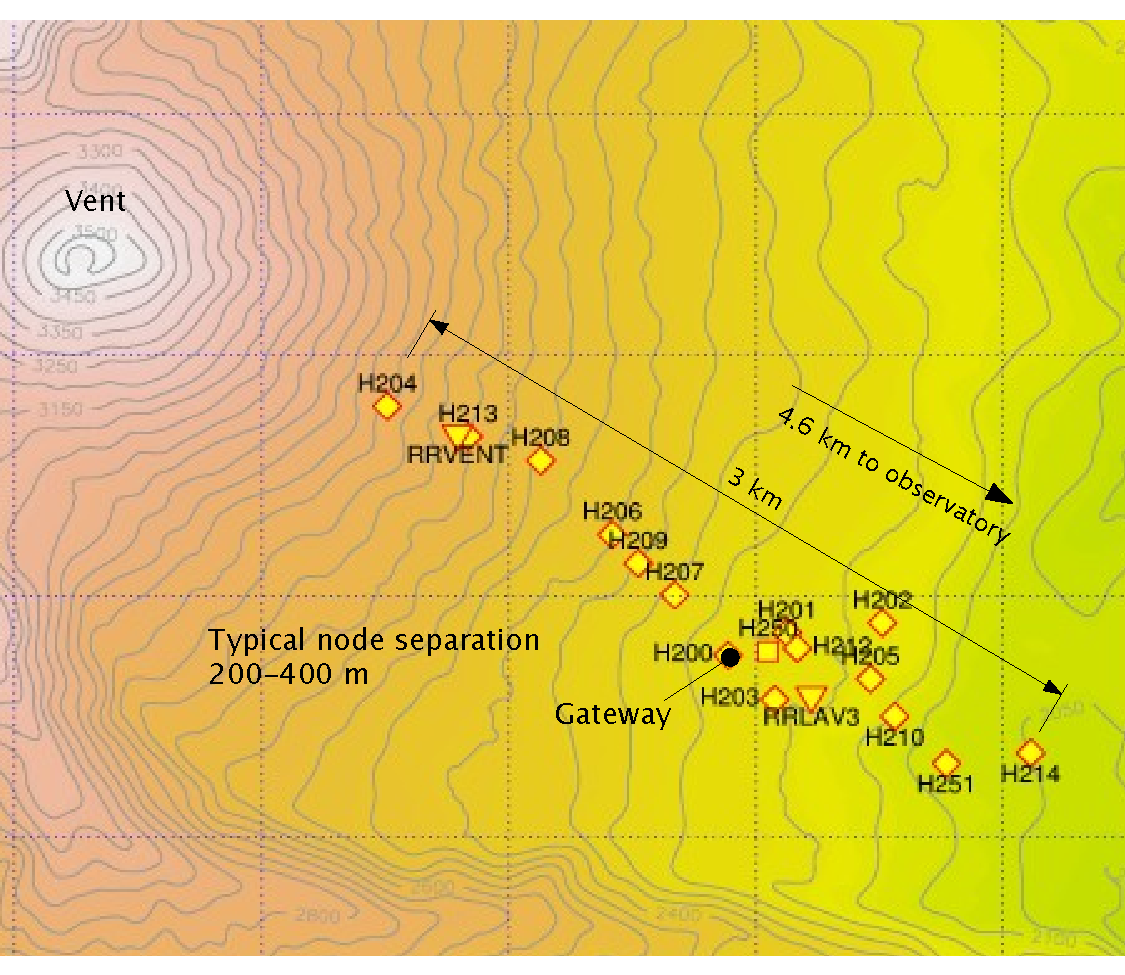
\includegraphics[width=1.0\hsize]{./5-evaluation/figs/pics/reventador-map-crop.pdf}
\end{center}
\caption{\textbf{Map of sensor deployment at Volc\'{a}n Reventador.}
In addition to the 16~sensor nodes, two broadband seismometers
with data loggers (RRVENT and RRLAV3) were colocated with the network.}
\end{figure}

% MDW 26-Aug-06: I have revisited some of Jeff Johnson's suggestions
% in the below text; i.e., hyphenation on "broad-band" and so forth.

Our deployment at Reventador took place between August 1--19, 2005.
Reventador is an active volcano located in northern Ecuador, about 100~km
from Quito. 
%The volcano erupted with massive force in 2002, blanketing the streets of
%Quito with ash, closing schools and the airport. 
During this time, Reventador's activity consisted of small explosive events
that ejected ash and incandescent blocks several times a day. Associated
seismicity included numerous explosion earthquakes as well as
extended-duration shaking (tremor) and shallow rock-fracturing earthquakes.

We deployed 16~sensor nodes on the upper flanks of Reventador, as shown in
Figure~\ref{evaluation-fig-map}, over a 3~km linear configuration radiating
away from the vent. The resulting multihop topology is shown in
Figure~\ref{evaluation-fig-schematic}. The upper flanks of the volcano were
completely deforested by a large eruption in November 2002, allowing for
line-of-sight radio communication between adjacent sensor nodes.  Two
standalone seismic stations, consisting of a broadband sensor, a Reftek 130
data logger with 1~GByte flash memory cards, and a GPS receiver for
timestamping, were colocated with sensor nodes. The data from these stations
is essential to our network validation, described in
Sections~\ref{evaluation-sec-eventdetection}~and~\ref{evaluation-sec-timing}.
The base station was located at a small hotel 4.6~km from the deployment
site.  The sensors were deployed for a total of 19~days, during which time
the network recorded data from 229~earthquakes, eruptions, and tremor events,
logging 107~MBytes of data. The long hike and lack of roads prevented
frequent returns to the deployment site, although we returned several times
to change batteries and perform other network maintenance.

%Colocated with our
%sensor network were two broadband seismometer stations,
%each using a Reftek~130 data logger with 1~GByte flash memory cards
%and a GPS receiver for timestamping. The data from these stations 
%is essential to our network validation, described in 
%Sections~\ref{sec-eventdetection}~and~\ref{sec-timing}.  
%The base station was located at 
%a small hotel 4.6~km from the deployment site. 

% MDW 26-Aug-06: I don't think this subsection is really needed. 
% Maybe the first paragraph could be added back somewhere; the rest is
% not pithy enough to warrant inclusion.

%\subsection{Design decisions}
%
%For this deployment our primary design goals were simplicity,
%statelessness, and robustness.  As such, we chose not to focus on
%aggressive power management, routing performance, fault tolerance
%(e.g. multiple base stations and GPS receivers), or scalability.  We
%plan to address these issues in future deployments.
%
%Some of our design decisions were influenced by the fact that the deployment
%site was a strenuous 3~hour hike from the observatory, meaning that we wanted
%to avoid problems that might require returning to the deployment
%site.  Other decisions were driven by more pragmatic reasons.  For example,
%although having a GPS receiver on each node would make the system more
%robust, we decided against it due to the increased cost, power, and
%deployment logistics.  Each GPS node requires a car battery to power it for a
%longer duration, making the deployment impractical given the difficult
%circumstances.  Instead we decided to equip only one node with a GPS receiver
%and use FTSP~\cite{ftsp} to synchronize the rest of the network.
%
%Finally, we point out that initially we planed on a 25~node network.
%However, because of various hardware failures we ended up with 16
%deployable nodes.


\section{Network Robustness}
\label{evaluation-sec-robustness}

The first evaluation metric that we consider is the {\em robustness} of the
sensor network.  Sensor network deployments have typically been plagued by
failures of individual nodes and the support infrastructure. Clearly,
robustness has a direct effect on the resulting data yield.  Our evaluation
shows that while nodes exhibited very high uptimes, the base station
infrastructure was very unreliable, and a single bug affecting the Deluge
protocol caused a three-day outage of the entire network.

%For example, in the 2003~Great Duck Island
%deployment~\cite{gdi-sensys04}, burrow nodes in the multihop network 
%failed after an average of 29~days, primarily due to battery
%exhaustion.

\subsection{Overall network uptime}

\begin{figure}[t]
\label{evaluation-fig-nodesalive}
\begin{center}
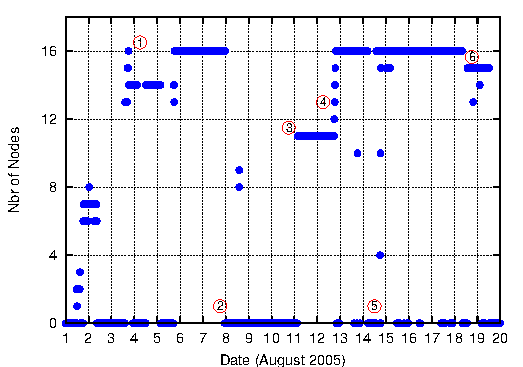
\includegraphics[width=\hsize]{./5-evaluation/figs/robustness/nodesalive/nodesalive.pdf}
\end{center}
\caption{\textbf{Nodes reporting over time.}
This figure shows the number of nodes reporting over each 10~min window
during the 19-day deployment period.  The annotations (1) through (6) are
described in the text.}
\end{figure}

Figure~\ref{evaluation-fig-nodesalive} shows the number of nodes reporting
over each 10-minute interval during the entire 19-day deployment. A node is
included in the count if any of its status messages were received at the base
station during the 10-minute window.  Annotations show several significant
events that occurred during the deployment. The network was installed in two
phases of 8~nodes each, the first on August~1 and the second on August~3.  At
label (1) the entire 16~node network is operational.  However, initial
software misconfiguration required rebooting several nodes during a third
visit to the deployment site on August~5.  The network then ran with 16~nodes
active for a little more than 2~days. 

At label (2) on August~8, a software command was transmitted to reboot the
network, using Deluge~\cite{deluge}, in an attempt to correct the time
synchronization fault described in Section~\ref{evaluation-sec-timing}.  This
caused a software failure affecting all nodes, with only a few reports being
received at the base station later on August~8.  After repeated attempts to
recover the network, we returned to the deployment site on August~11 (label
(3)) to manually reprogram each node.  However, only 11~nodes could be
reached before nightfall, forcing a return to the observatory. On August~12
(label (4)) we returned to the deployment site and reprogrammed the remaining
5~nodes. 

From August~13~through~18, all~16~nodes were reporting nearly continuously.
The intermittent failures (label (5)) were caused by power outages at the
observatory, causing the base station laptop and radio modem to fail. During
these times no data was logged by the base station although the sensor nodes
themselves were probably operational, since all nodes would report when the
base station recovered.

Several days before the end of the deployment, node 204, located closest to
the vent, stopped reporting data (label (6)). When the network was
disassembled we discovered that the antenna mast had been destroyed, most
likely by a bomb ejected from the volcano during an eruption, although the
node itself remained intact.  This failure underscores the importance of
remote telemetry for acquiring data at hazardous volcanoes.

\subsection{Individual node uptime}

\begin{figure}[t]
\label{evaluation-fig-nodeuptime}
\begin{center}
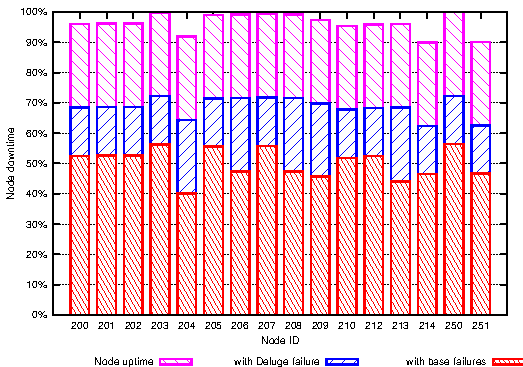
\includegraphics[width=\hsize]{./5-evaluation/figs/robustness/nodesalive/node-uptime2.pdf}
\end{center}
\caption{\textbf{Individual node uptimes.}
This figure shows the percentage of time that each node reported status
messages during the 19-day deployment.  Shown separately are the apparent
node uptimes caused by the whole-network outage and base station outages.
While the former was true sensor node failure, the latter did not seem to
affect the sensor nodes themselves.}
\end{figure}

Figure~\ref{evaluation-fig-nodeuptime} shows the uptime for each node during
the 19-day deployment. Each bar consists of three portions. The lowest
portion is the {\em apparent} uptime of each node accounting for both the
base station failures and single 3-day~software outage. Because base station
failures did not affect individual nodes, the middle bar shows the apparent
uptime including only the 3-day~outage. In this case, the mean node uptime
is~69\%.  However, with the 3-day outage factored out, nodes achieved an
average uptime of~96\%.  These numbers are encouraging and suggest that the
sensor nodes were very reliable in spite of the software crash.

Based on discussions with the authors of Deluge, we believe this failure was
caused by a single bug in the {\tt InternalFlash} TinyOS component (which has
since been fixed).  This bug prevented Deluge from storing critical state
information, causing nodes to reboot continuously at short intervals.  We did
not see this behavior in the lab before deployment, although we had not
rigorously tested this portion of the code. In retrospect, it was optimistic
of us to rely on a complex network reboot protocol that had not been
field-tested.  Deluge was removed from the binary used during the network
reprogram following the failure; it was replaced with a simpler mechanism to
reboot individual nodes using a radio command.

%  - Node reboots [KL]
%    - Determine manual vs. automatic reboots
%    - Correlate reboots to other node properties (routing load?)
%    - Impact of reboot (latency)
%\begin{figure}[t]
%  \begin{center}
%    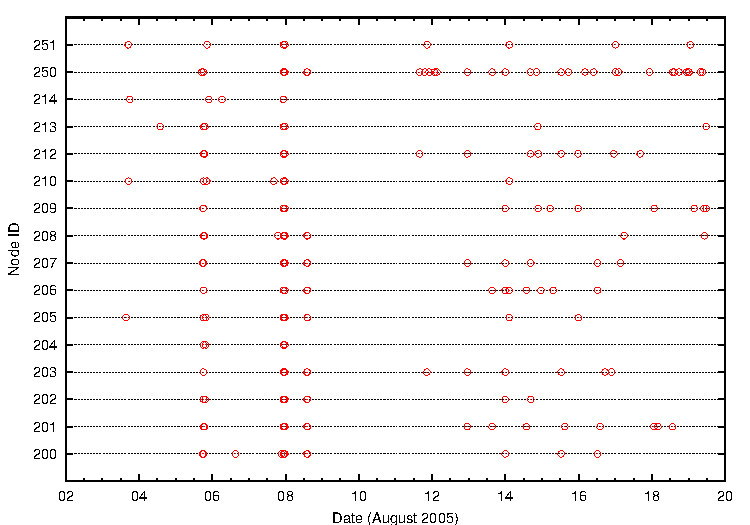
\includegraphics[width=\hsize]{./5-evaluation/figs/robustness/nodeReboots/nodeReboots.pdf}
%  \end{center}
%  \caption{\small{\bf Reboots of each node}
%    {\em This figure shows when each node rebooted during the 19-day deployment.}}
%    \label{fig-nodeReboots}
%\end{figure}


%\begin{figure}[t]
%  \begin{center}
%    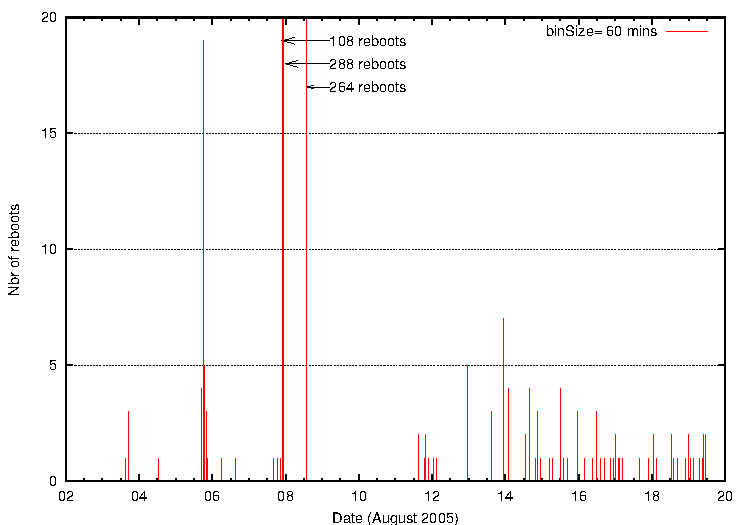
\includegraphics[width=\hsize]{./5-evaluation/figs/robustness/nodeReboots/nodeRebootsBinned.pdf}
%  \end{center}
%  \caption{\small{\bf Number of reboots over time}
%    {\em This figure shows a the number of reboots in 60 minute
%    windows.  As we can see, there was an unusually large number of
%    reboots right before the network reprogramming.}}
%    \label{fig-nodeRebootsBinned}
%\end{figure}

\subsection{Discussion}

Failures of the base station infrastructure were a significant source of
network downtime during the deployment.  This contrasts with common
assumptions that the base station is generally reliable and operating on a
continuous power source. This was our expectation prior to the deployment,
and we did not make adequate preparations for the intermittent electrical
supply at the observatory. A backup diesel generator was used during nightly
power outages, with extra laptop and car batteries supplying power when it
failed.  However, this approach was not ultimately successful.

It may be surprising that node uptime is not related to depth in the routing
tree. This suggests that if a node is ``down'' (i.e., we do not receive any
status messages from it during a 10-minute window) that it is still active
and routing packets for its children in the tree, even as its own status
messages are being lost. An alternate explanation is that a node could select
an alternate parent in the routing topology when its parent fails. However,
our analysis of the routing topology does not support this view, since nodes
rarely use more than one parent. For example, node~214 \textit{always} routes
data through node~251. The volcano-induced failure of node~204 near the end
of the deployment is the only notable failure of a single node.


\section{Event Detector Accuracy}
\label{evaluation-sec-eventdetection}

Our network was designed to capture interesting volcanic signals.  Thus, it
is critical that the system correctly identify and report such events.  This
section evaluates our event detection algorithm both in terms of the number
and rate of event triggers as well as its ability to detect scientifically
interesting events.

\subsection{Event triggers per node}

\begin{figure}[t]
\label{evaluation-fig-eventspernode}
\begin{center}
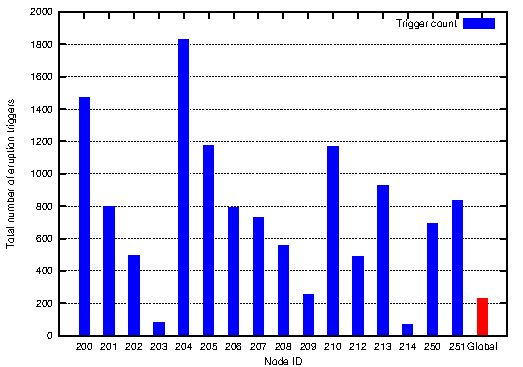
\includegraphics[width=\hsize]{./5-evaluation/figs/eventdetection/eruptionTriggers/eruptCount.pdf}
\end{center}
\caption{\textbf{Event triggers per node.}
This figure shows the total number of event triggers reported by each node.
It demonstrates a wide variation in trigger rates that cannot be attributed
only to varying node uptimes. For example, node~204 had the lowest uptime but
the largest number of event triggers.}
\end{figure}

\begin{figure}[t]
\label{evaluation-fig-eventspertime}
\begin{center}
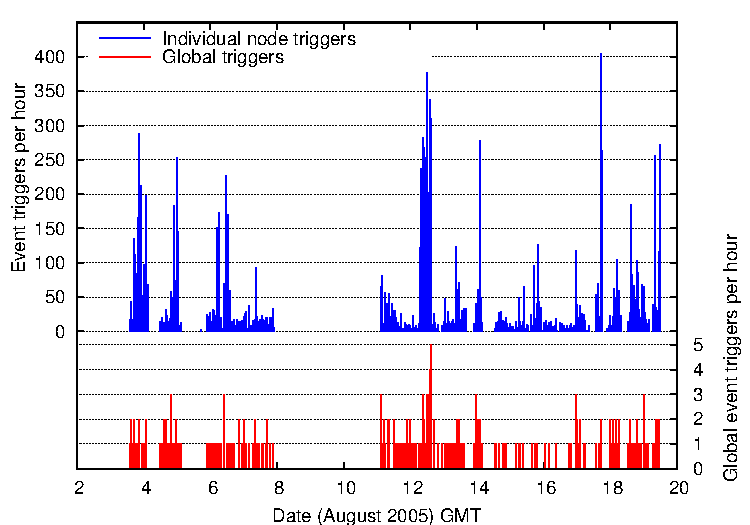
\includegraphics[width=\hsize]{./5-evaluation/figs/eventdetection/eruptionTriggers/eruptCountVsTime.pdf}
\end{center}
\caption{\textbf{Event triggers over time.}
The upper graph shows the total number of individual node triggers per hour.
The lower graph shows the corresponding number of global triggers.
Reventador's varying seismic activity generated between 0~to~5 global
triggers per hour.}
\end{figure}

Figure~\ref{evaluation-fig-eventspernode} shows the total number of events
reported by each node during the deployment. It shows a wide variation in the
event trigger rate, from 70~triggers for node~213 to 1830~triggers for
node~204.  Variation in the trigger rate can be attributed to many factors,
including the location of the node, the orientation of the seismometer, and
the quality of the seismometer-to-ground coupling.  Note that the trigger
rate does not seem to be related to distance from the vent. Although node~204
was closest to the vent and reported the most triggers, nodes 200, 205, and
210 all had high trigger counts despite being significantly farther away.

\subsection{Event triggers over time}

Figure~\ref{evaluation-fig-eventspertime} shows both the number of individual
node and global event triggers over each hour. We observe that the volcano's
activity varied greatly, generating trigger counts ranging between~2~and~405
events per hour when the network was online.  This activity translates into
up to 5~global event triggers an hour, each initiating a Fetch download cycle
of the associated data.

The volcano's bursty and unpredictable activity makes the network's design
more challenging than systems designed for statically-scheduled data
collection.  The data collection protocol, based on our earlier deployment at
Tungurahua~\cite{volcano-ewsn05}, assumed that events would be rare and that
it would be unnecessary to simultaneously record signals for one event while
downloading another. As a result, we missed a number of impressive
back-to-back eruptions typical of the activity at Reventador. It is worth
noting that the variable number of event reports is itself a measure of the
volcano's activity level and could be used to assess hazard levels. 

\subsection{Event detector accuracy}
\label{sec-eventdetectaccuracy}

%  - Event detector accuracy vs. Reftek data [MDW]
%    - Vary E.D. parameters

The network detected 229~eruptions, explosions, earthquakes, and tremor
events during the deployment. Ideally, we would like to assess its accuracy
in terms of the fraction of true events detected, as well as the false
positive rate. Given the high degree of coherence required by the global
event detector (requiring 30\% of the active nodes to trigger within a short
time window), we would be surprised if the sensor network recorded any false
events. Indeed, all of the signals we did capture appear to be based on true
volcanic activity, indicating a zero false positive rate.

We intended to apply our event detection algorithm to the signals collected
by the two broadband seismic stations to establish the algorithm's accuracy.
Unfortunately, we found this to be difficult for several reasons.  First,
each of the broadband stations suffered intermittent power and software
failures, either preventing them from logging any data, or corrupting the
collected signals or timestamps.  Thus, even in those cases where broadband
data is available, it is not always accurate. 
%Moreover, intermittent noise on a single broadband station could be
%interpreted as an event by our algorithm, yielding an artificially high
%trigger rate. 
Second, the broadband stations deployed a more sensitive seismometer with a
much wider frequency response.  The geophones used by our sensor nodes have a
corner frequency of 4.5~Hz, while the broadband sensors have a corner
frequency of 0.033~Hz.  Additionally, the broadband seismometers are much
more sensitive, generating voltages of 800~V/m/sec, whereas the geophones
have a sensitivity of only 32~V/m/sec. As a result, the broadband sensors are
able to detect much weaker seismic signals.

We focus our attention on a single day of data where the broadband stations
were recording clean data and the sensor network was relatively stable. One
of the authors, a seismologist, visually extracted events from the broadband
data; during this 24-hour period, a total of 589~events were recorded by the
broadband sensors. During the same time, the sensor network triggered on just
7~events, suggesting that our detection accuracy is very low (about 1\%).

The network could have failed to detect a seismic event for one of four
reasons: (1) failure of individual nodes; (2) failure of the base station or
radio modem; (3) the low sensitivity of our seismometers; or (4) failure of
the event detection algorithm itself. To factor out the increased sensitivity
of the broadband seismometers, we only consider the 174~events with SNR~$\geq
10$ from both stations, which we expect the geophones should have been able
to detect as well.  Also, Section~\ref{evaluation-sec-robustness} has already
addressed the question of uptime, so we focus here on the inherent accuracy
of the event detector when the network was operating correctly. 136~of the
174~broadband events occurred during times when the network was operational.
Taking these two factors into account, the network's detection accuracy is
still only about 5\%. 

%It is not
%clear how to tune the event detection algorithm for the broadband data.
%If the algorithm is not sensitive enough, it will fail to detect events that
%our network did in fact report.  If the algorithm is too sensitive, it will
%report false events that the sensor network should not have reported. 
%Although our EWMA-based algorithm was developed after consultation
%with seismologists, there is no single gold standard for event detection in
%the volcanological community.
%However, we did not experiment with different event-detection parameters in
%the field, as the number of eruptions and earthquakes triggering the current
%detector was more than adequate to exercise the network.  For our deployment
%the sheer volume of data precludes manual selection of events.

%In an attempt to assess the event detector's accuracy, we
%applied our original event-detection algorithm to the filtered 
%broadband data from August~11--19, which corresponds to 143~events 
%captured by our sensor network. 75~out of these~143 events (52\%) 
%have a trigger from at least one broadband station; 47~events (32\%)
%have triggers from both stations. The lack of triggers for the 
%remaining events (all of which are true seismic activity) 
%is due to corruption or gaps in the broadband data. 

%143~events from August 11--19 which were properly time rectified as described
%in Section~\ref{sec-timing}.  Of these events, 142 had corresponding data
%from at least one broadband station.  We then ran the original event
%detection algorithm on the broadband signals.
%%In addition, we lowered the EWMA ratio threshold of the detector from 1050
%%to 1030, making the detector much more sensitive than the mote detector.
%Due to the small number of broadband stations we consider a trigger from 
%{\em either} station as identifying a meaningful event. This implies that
%noise on a single station can increase our false positive rate.

% PARAMETERS USED HERE:
%   - Broadband event detector: low gain 1.0, high gain 9.0, threshold 1050
%   - Vote count required: 1 
%   - No suppression
%This resulted in 12505~individual triggers from the broadband data.
%123~out of the~142~events (87\%) had a
%corresponding trigger in the broadband data.  
%Given the high degree of
%coherence required by the global event detector (requiring 5~nodes to
%trigger within a short time window), we would be surprised if the sensor
%network recorded any spurious events. Indeed, all of the signals we did
%capture appear to be based on true volcanic activity.  
%We suspect that the
%lack of triggers for the remaining 19~events is due to corruption in the
%broadband data.
%However, with only 3~broadband stations, any one of
%which could have been faulty at any time, it is difficult to use this
%data to definitively evaluate event detection accuracy. 

%%%%%%%%%%%%%%%%%%%%%%%%%%%%%%%%%%%%%%%%%%%%%%%%%%%%%%%%%%%%%%%%%%%%%%%%%%%%
%%% MDW: Original text here:
%The more difficult question is what fraction of ``true'' events were
%successfully detected. As discussed above, without a gold standard for event
%detection and complete broadband data coverage, it is impossible to make 
%a direct comparison. The best we can do is use our original 
%event-detection algorithm on the broadband data and compare the 
%set of triggers to those reported by our network.
%
%Using the same global detector parameters (requiring both broadband
%stations to trigger within a 10~sec window) 
%yields 285 events in the broadband data set.
%%(a significant reduction from the 12505 individual triggers, suggesting very
%%high noise in the broadband data).
%Of these, 36 events (13\%) correspond to events recorded by our network.
%Each of remaining 249 missing events is the result of either the failure of
%the event detector, the failure of the sensor network, or false positives
%in the broadband data set. With only two broadband stations it is
%difficult to tease these reasons apart.  Of the 136 broadband events that
%occurred while all 16~nodes of the sensor network were operational, our
%network detected~24. If the broadband stations are considered ground truth
%this results in a detection accuracy of 17.7\%. 
%%%%%%%%%%%%%%%%%%%%%%%%%%%%%%%%%%%%%%%%%%%%%%%%%%%%%%%%%%%%%%%%%%%%%%%%%%%%

%%%%%%%%%%%%%%%%%%%%%%%%%%%%%%%%%%%%%%%%%%%%%%%%%%%%%%%%%%%%%%%%%%%%%%%%%%%%
%%% MDW: New text here:

%Without complete broadband data coverage, there is no way to tell how
%many true events occurred.  For sake of argument, let us consider the set
%of seismic events triggered in {\em both} broadband stations, a total
%of 406~triggers, as ``ground truth.''  However, because there are only
%two broadband stations, we expect a high false positive rate in the
%broadband data.  For example, if we had required only two~sensor votes 
%to trigger (rather than five), the number of sensor node events jumps 
%from 70~to~462 (an increase of 660\%) suggesting that the broadband
%trigger rate is artificially high.

%To compare the sensor network and broadband triggers, 
%We dilate each broadband trigger by 60~sec and consider
%any sensor network trigger that falls within this window to be 
%a match. 27~out of~the~70~(38\%) sensor network triggers match some 
%broadband trigger. Combining the broadband and sensor network
%triggers, there are 449~unique events; the sensor network detected 6\%. 
%However, it is worth noting
%that the broadband station missed 43~of the 70~sensor network events,
%likely due to missing data. The fact that the
%sensor network and broadband triggers are poorly correlated
%suggests that using the broadband stations is not an accurate 
%measure of ground truth. 

Recall that during a Fetch download cycle, nodes disabled sampling to avoid
overwriting data in flash. Download cycles could take up to several minutes
{\em per node} (see Section~\ref{evaluation-sec-performance}), meaning that
there are significant time windows when the network was unable to detect new
events.  During the Fetch cycles on August 15, the broadband stations
recorded 42~events, 24\% of the total events detected.  This indicates that,
all else being equal, the sensor network could have detected approximately
24\% more events had we designed the protocol to sample and download
simultaneously. We plan to add this feature in the next version of our
system.

In the end, we believe that our low detection rate is the result of the
parameters used in the EWMA-based event detection algorithm.  These
parameters were chosen prior to the deployment, based on our experience with
detecting infrasonic events at a different volcano~\cite{volcano-ewsn05}. We
did not experiment with modifying them in the field. Indeed, using our
algorithm with these same parameters on the broadband data for August~15
detects only 101~events, a fraction of the events chosen manually by an
expert.  We plan to tune our event-detection parameters for future
deployments based on the data collected by the broadband stations.

%Because we cannot define ground truth in absolute terms, we cannot
%directly report on the specificity and sensitivity of our event detection
%algorithm. Instead, we verify that for each event recorded by the
%sensor network, the same event-detection algorithm applied to the
%corresponding broadband station data would have also reported an 
%event. This is a measure of how many ``false positives'' are reported
%by the sensor network but does not capture ``false negatives.''
%
%We took a representative set of 78~events that appear to have accurate 
%timing (as described in Section~\ref{sec-timing}). We then applied our
%original event-detection algorithm on the corresponding data from 
%the RRVEN and RHOTEL stations (eliding station RLAV3 for the reasons 
%described above). The same event-detection parameters were used as
%by the motes in the original deployment. As expected, the algorithm 
%applied to the broadband data triggered events in 100\% of these cases, 
%meaning that there are no false positive events in our data set.

%less consensus about what constitutes a ``real event.''
%It is an open question what proportion of ``true'' events we
%successfully captured. 

%Applying our
%original algorithm to the broadband data set for August 11--19 
%reports 315~unique events. During the same period the sensor network
%reported 144~events. Only 33 events, or 23\% of the events reported
%by the network, match in both data sets. This is due to many factors.

%\begin{figure*}[t]
%\begin{tabular}{|llllll|} \hline
%{\bf Suppression window} & 
%{\bf Broadband events} &
%{\bf Mote events} &
%{\bf Matching events} & 
%{\bf ``False positive'' \%} & 
%{\bf ``False negative'' \%} \\ \hline
%{\bf 1 votes needed, thresh 1050} & & & & & \\ \hline
% {\em none}	& 8031 & 144 & 89 & 38\% & 99\% \\  \hline
%{\bf 2 votes needed, thresh 1050} & & & & & \\ \hline
% {\em none}	& 3530 & 144 & 37 & 74\% & 99\% \\  \hline
%\end{tabular}
%\caption{\small \XXXnote{finish this!}}
%\end{figure*}
%
%  - Global detector accuracy [MDW]
%    - How well did global detector filter out false events
%    - Specificity/sensitivity analysis [MDW - hold off]



\section{Data Collection Performance}
\label{evaluation-sec-performance}

In this section we assess the performance of the {\em Fetch} data collection
protocol. We evaluate Fetch in terms of its {\em yield}, its ability to
successfully collect requested data; and its {\em latency}, the time to
download events from the network.

\subsection{Data yield}

We define the {\em event yield} of a Fetch transfer as the fraction of nodes
for which the entire 60~sec signal was successfully downloaded following an
event. The calculation only considers those nodes that were active at the
time of the event detection (Figure~\ref{evaluation-fig-nodesalive}).  For
example, if 10~nodes were active during an event, then the event yield is
defined in terms of 10~nodes.  Note that the Fetch protocol attempts to
download a signal from all active nodes, even those that did not detect the
event.

\begin{figure}[t]
\label{evaluation-fig-compBlockYieldCDF}
\begin{center}
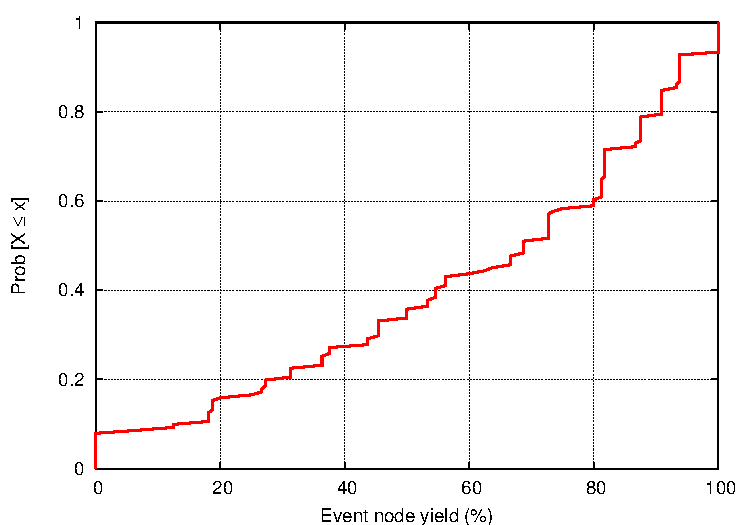
\includegraphics[width=\hsize]{./5-evaluation/figs/performance/yields/comparison/availableEventNodeYieldCDF.pdf}
\end{center}
\caption{\textbf{vent yield.}
This graph shows a CDF of the event yield for each of the 229~events recorded
during the entire deployment. Event yield is the fraction of active nodes
from which a complete 60~sec signal was downloaded following an event.}
\end{figure}

Figure~\ref{evaluation-fig-compBlockYieldCDF} shows a CDF of the event yield
for all 229~events recorded during the deployment.  As the figure shows, the
median event yield was 68.5\% and the 90th percentile was 94\%.  The yield
can be affected by several factors.  First, the protocol will abort a
transfer from a node after re-requesting the same block more than 20~times,
or if the transfer from a single node exceeds 10~minutes.  Second, because
sampling is disabled while performing a data transfer, if two back-to-back
events occur a node may not end up storing data for the second event.


% ------ Original text ------------------------
%% In this section we assess the performance of the {\em Fetch} data collection
%% protocol. We evaluate Fetch in terms of its {\em yield}, its ability 
%% to successfully collect requested data; and its {\em latency}, the 
%% time it took to download events from the network.

%% \subsection{Data yield}
%% %  - Yield [KL]
%% %    - % of detected events that we successfully downloaded data for
%% %    - How much data per event
%% %    - Consider all nodes vs. only "active" nodes
%% %    - Before and after reprogram

%% We define the {\em event block yield} of a Fetch transfer as the fraction of
%% requested data blocks successfully downloaded from each node following an
%% event. The calculation only considers those nodes that were operational at
%% the time of the event detection. For example, if 10~nodes were active during an
%% event, then the event block yield is defined as the fraction of data blocks
%% retrieved from those 10~nodes.  Normally, following an event the system would
%% attempt to download 60~sec of data from each operational node, including
%% nodes that did not report the event. 

%% \begin{figure}[t]
%% \begin{center}
%% 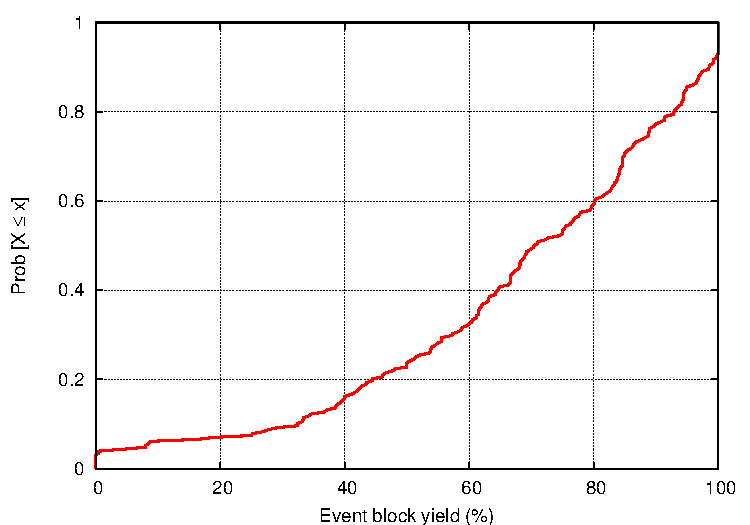
\includegraphics[width=\hsize]{./5-evaluation/figs/performance/yields/comparison/schBlockYieldCDF_entire.pdf}
%% \end{center}
%% \caption{\small{\bf Event block yield.}
%% {\em This graph shows a CDF of the event block yield for each of the 229~events
%% recorded during the entire deployment.}}
%% \label{fig-compBlockYieldCDF}
%% \end{figure}

%% Figure~\ref{fig-compBlockYieldCDF} shows a CDF of the event block
%% yield for all 229~events recorded during the deployment.  As the
%% figure shows, the median event block yield was 70.4\% and the 90th
%% percentile was 98.6\%.  The yield can be affected by several factors.
%% First, the protocol will abort a transfer from a node after
%% re-requesting the same block more than 20~times, or if the transfer
%% from a single node exceeds 10~minutes.  Second, because sampling is
%% disabled while performing a data transfer, if two back-to-back events
%% occur a node may not end up storing data for the second event.
% --------------------------------------------------------


%The event block yield of each transfer is affected by several factors.
%First, the Fetch protocol will timeout on a transfer from a node after
%re-requesting the same block more than 20~times, or if the cumulative
%transfer time from a single node exceeds 10~minutes.	Second, the protocol
%may request blocks not in a node's cache.  Because we disable sampling during
%a Fetch transfer, if two back-to-back events occur the second Fetch operation
%may attempt to request blocks that the node never stored because it was busy
%with the first transfer. Or we may simply fail to disable sampling on a
%particular node causing the requested blocks to be overwritten before we are
%able to retrieve them. 

%Also shown is a breakdown of the
%event block yield both before and after the network was reprogrammed on
%August 11, 2005 following the Deluge failure. After the
%reprogramming, the median event block yield improved from 66.7\% to 77.8\%. 

%The improvement is due to several changes that were introduced
%following the reprogramming in an attempt to improve the performance
%and robustness of the Fetch protocol based on our observations in the
%first few days of the deployment.  First, the transfer timeout was
%increased from 10~minutes to 20~minutes, giving nodes more time to
%respond to Fetch requests. Second, the speed at which Fetch commands
%were propagated through the network was increased by a factor of~4,
%decreasing the latency for a Fetch request to reach a node.  Third, we
%disabled duplicate suppression in the flooding protocol used to
%propagate Fetch requests to the network, increasing overall network
%load but increasing reliability.

%Figure~\ref{fig-compNodePercentiles} shows the 50th-percentile yield
%for each node before and after network reprogramming.  The yield for
%most nodes is very good (100\% in most cases), with a couple of
%exceptions.  In general, the yield is highest for nodes that were
%closest to the root of the tree and for those that only had 2
%channels.  This is consistent with our expectations.  When the base
%station concludes that there was an event, it first floods the network
%with a command telling nodes to stop sampling.  Afterwards, it
%downloads the event data from each node in a round-robin fashion,
%ordered by hop count from the root.  We observed that the stop
%sampling message did not always propagate to all the nodes, with nodes
%farter away from the root beeing less likely to have received the stop
%sampling command.  If a node did not stop sampling, there was a good
%chance that it might have overwritten it's circular flash buffer by
%the time it was scheduled to be downloaded.  Again this is more likely
%for nodes farter away because they were scheduled later.  The two
%nodes with 4 channeles, 250 and 251, produce twice as much data than
%the 2-channel nodes and therefore fill in their falsh at twice the
%rate.  Note that node 251 was also the second farthes node from the
%root after node 214.
%
%In Figure~\ref{fig-compNodePercentiles} we also see that after the
%network reprogramming, the yield for each node improved or stayed the
%same.  \XXXnote{add explanations}.

%\begin{figure}[t]
%\begin{center}
%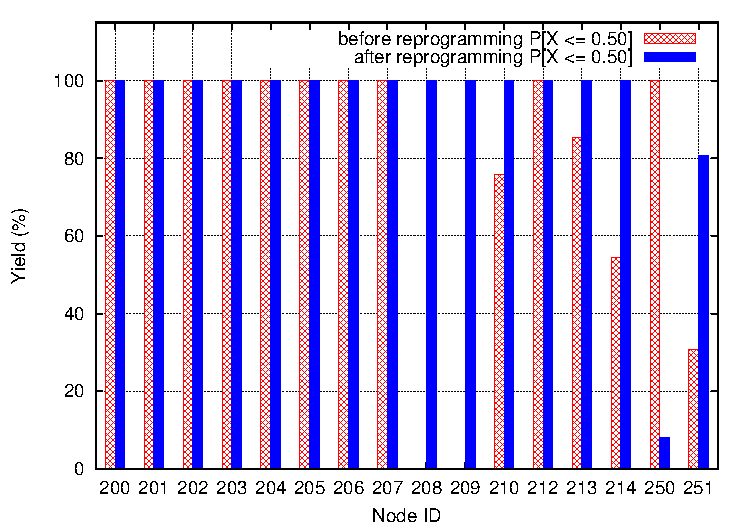
\includegraphics[width=\hsize]{./5-evaluation/figs/performance/yields/comparison/nodePercentiles.pdf}
%\end{center}
%\caption{\small{\bf 50th-percentile yield by nodeID before and after network reprogramming.}
%{\em The 50th-percentile yield for most of the nodes is very good,
%with a few exceptions.  After the network reprogramming, the yield for
%all nodes either improved or stayed the same.}}
%\label{fig-compNodePercentiles}
%\end{figure}

%% \XXXnote{MDW: The previous definition of ``node yield'' did not make
%% sense to me. I have tried to reword this but Konrad needs to check
%% that this is right. It does not make sense to ``download a node.''}

Next, we look at the {\em node yield} which we define as the probability that
an event was successfully downloaded from a given node.  Like the event
yield, the calculation only considers those nodes that were active at the
time of each event detection.  Node yield can be affected by several factors.
The depth and radio link quality of a node's routing path to the base station
affect packet loss rate and thereby the likelihood of a Fetch timeout.
%The farther a node is from the root of the tree, and the more low-quality
%links it has to route across, the more likely its packets will get lost.  
Additionally, two nodes outfitted with triaxial seismometers
(nodes~250~and~251) sample and store twice as much data as the others,
increasing the probability of a timeout.  Finally, a bug in our control
application caused node~250 to sample data continuously, even during a Fetch
operation. As a result, this node was more likely to overwrite an event
stored in flash before it could be downloaded.

\begin{figure}[t]
\label{evaluation-fig-nodeYield}
\begin{center}
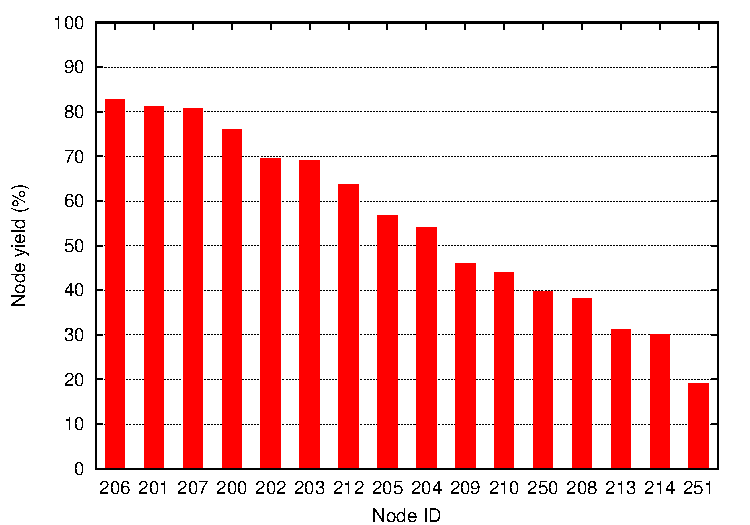
\includegraphics[width=\hsize]{./5-evaluation/figs/performance/yields/nodeYield/nodeYieldOnly.pdf}
\end{center}
\caption{\textbf{Node yield.}
This graph shows the node yield for each of the 16 nodes over the entire
deployment, defined as the probability that an event was successfully
downloaded from a node, as long as that node is active during the
corresponding event detection.}
\end{figure}

%% \XXXnote{MDW: I am very confused by this figure and the terminology
%% here. What does ``the total number of times a node was available and
%% successfully downloaded'' mean? I think we should probably just
%% eliminate the extra bars from the figure here, and only show the node
%% yield by itself. We have already shown the node uptimes in another figure.}

Figure~\ref{evaluation-fig-nodeYield} shows the node yield for each of the
nodes.
%% For comparison, it also shows the total number of times a node was
%% available and successfully downloaded for the entire deployment.  
We can see how the factors mentioned above affected performance.  First, the
nodes with the highest yield (above 80\%) tend to be within two hops from the
root (see Figure~\ref{evaluation-fig-schematic}).  However, despite being
within two or three hops, node~209 had a fairly low yield.  This is explained
by the fact that node~209 had a poor link to its closest parent, node~200.
In fact, although most nodes had a stable parent throughout the deployment,
node~209 used node~200 as its parent only 33\% of the time and nodes
206~and~207 the remaining 66\% of the time.  Node~213 also switched parents
between nodes 204~and~208, but unlike node~209 it was always three hops away.
Node~214 was the farthest node in terms of hopcount and as a result had one
of the lowest yields.  The larger amount of data was also a factor for the
four-channel nodes, 250~and~251. In addition, node~251 was five radio hops
from the gateway.


% -------- Original text ---------------------------------------------
%% Next, we look at the {\em node block yield} which we define as the fraction
%% of requested data blocks successfully downloaded from each node.
%% The node block yield can be affected by several 
%% factors. The depth and radio link quality of a node's routing path 
%% to the base station affect packet loss rate and thereby the likelihood
%% of a Fetch timeout.
%% %The farther a node
%% %is from the root of the tree, 
%% %and the more low-quality links it has to route
%% %across, 
%% %the more likely its packets will get lost.  
%% Additionally, two nodes outfitted with triaxial seismometers
%% (nodes~250~and~251) sample and store twice as much data as the others,
%% increasing the likelihood of failure.  Finally, a bug in our control
%% application caused node 250 to sample data continuously, even during a Fetch
%% operation. As a result, this node was more likely to overwrite an 
%% event stored in flash before it could be downloaded.

%% \begin{figure}[t]
%% \begin{center}
%% 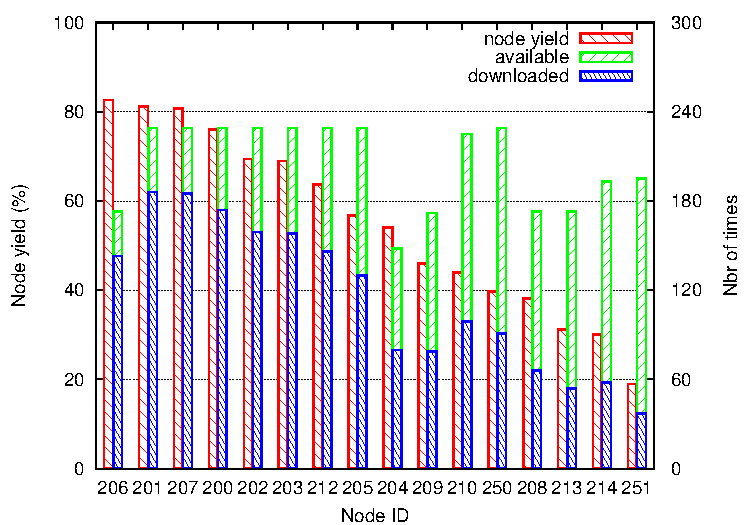
\includegraphics[width=\hsize]{./5-evaluation/figs/performance/yields/nodeYield/nodeYield.pdf}
%% \end{center}
%% \caption{\small{\bf Node block yield.}
%% {\em This graph shows the node block yield for each of the 16 nodes
%%   over the entire deployment. For comparison, the graph also shows the
%% total number of scheduled and downloaded blocks for each node on the 
%% right-hand $y$-axis.}}
%% \label{fig-nodeYield}
%% \end{figure}

%% Figure~\ref{fig-nodeYield} shows the node block yield for each of the nodes.
%% For comparison, it also shows the total number of blocks scheduled and
%% downloaded for the entire deployment.  We can see how the factors mentioned
%% above affected performance.  First, the blocks with the highest yield (above
%% 85\%) tend to be within two hops from the root (see
%% Figure~\ref{fig-schematic}).  However, despite being within two or three hops
%% node~209 had one of the lowest yields.  This is explained by the fact that
%% node~209 had a poor link to its closest parent, node~200.  In fact, although
%% most nodes had a stable parent throughout the deployment, node~209 used 
%% node~200 as its parent only 33\% of the time and nodes 206~and~207 
%% the remaining 66\% of the time.  
%% Node~213 also switched parents between nodes 204~and~208, but
%% unlike node~209 it was always three hops away.  Node~214 was the farthest
%% node in terms of hopcount and as a result had one of the lowest yields.  
%% The larger amount of data was also a factor for the four-channel nodes, 
%% 250~and~251. In addition, node~251 was five radio hops from the gateway.
% --------------------------------------------------------------


%% ; node 250 was continousely sampling, and therefore Fetch could not %
%always reach it before it overwrote the relevant data.

%% \begin{figure}[t]
%% \begin{center}
%% 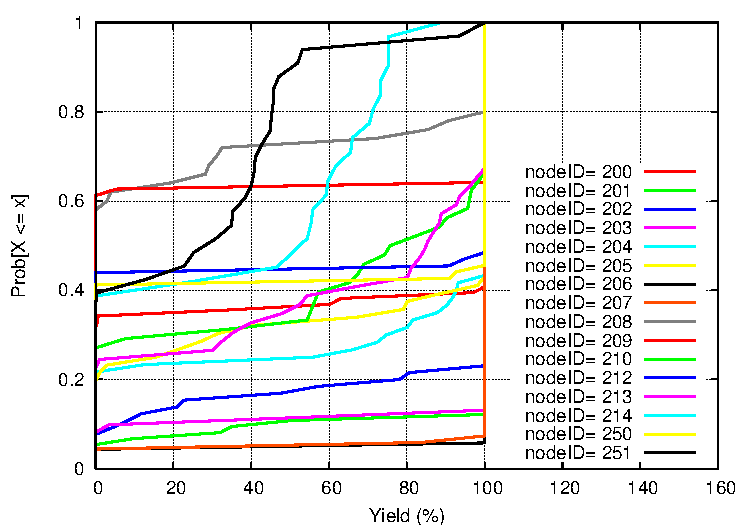
\includegraphics[width=\hsize]{./5-evaluation/figs/performance/yields/beforeReprogram/schBlockYieldCDFByNode.pdf}
%% \end{center}
%% \caption{\small{\bf Block yield by nodeID before network reprogramming.}
%% {\em This graph shows CDFs of the block yields for each node.  The
%% yields for some of the nodes is much higher (mostly the ones that were
%% farther in the routing tree) than for others.}}
%% \label{fig-blockYieldByNodeBeforeReprog}
%% \end{figure}

%% \begin{figure}[t]
%% \begin{center}
%% 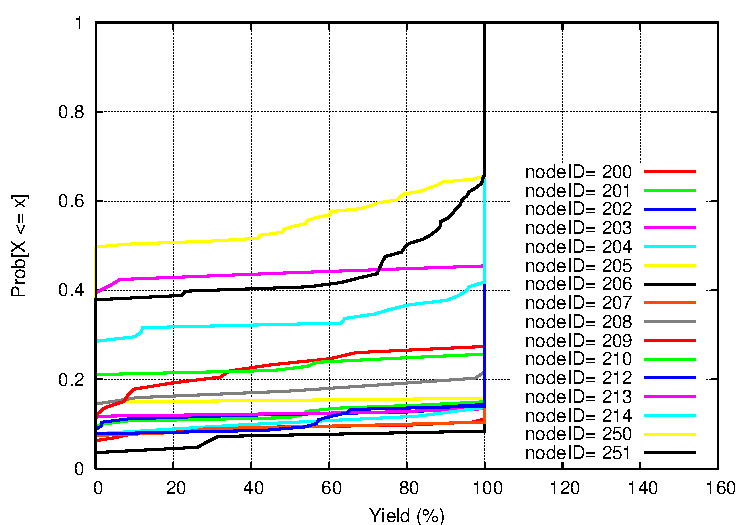
\includegraphics[width=\hsize]{./5-evaluation/figs/performance/yields/afterReprogram/schBlockYieldCDFByNode.pdf}
%% \end{center}
%% \caption{\small{\bf Block yield by nodeID after network reprogramming.}
%% {\em This graph shows CDFs of the block yields for each node.  The
%% yields for some of the nodes is much higher (mostly the ones that were
%% farther in the routing tree) than for others.}}
%% \label{fig-blockYieldByNodeAfterReprog}
%% \end{figure}


%% \begin{figure}[t]
%% \begin{center}
%% 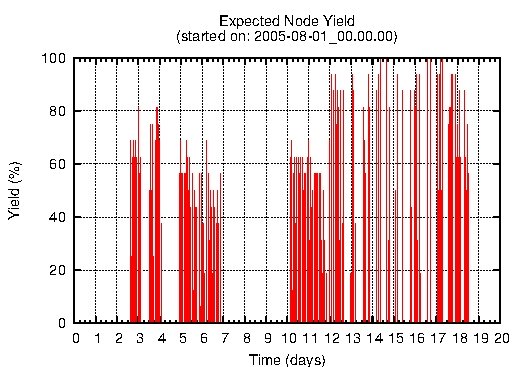
\includegraphics[width=\hsize]{./5-evaluation/figs/performance/yields/expNodeYield.pdf}
%% \end{center}
%% \caption{\small{\bf Expected node yield.}
%% {\em This graph shows the node yield out of the 16 nodes.  Only nodes
%% for which the enitre event was downloaded successfully are considered.}}
%% \label{fig-expNodeYield}
%% \end{figure}

%% \begin{figure}[t]
%% \begin{center}
%% 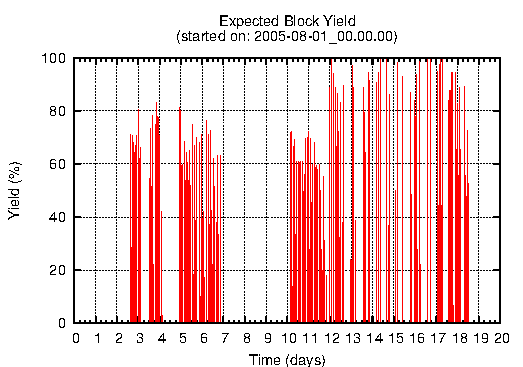
\includegraphics[width=\hsize]{./5-evaluation/figs/performance/yields/expBlockYield.pdf}
%% \end{center}
%% \caption{\small{\bf Expected block yield.}
%% {\em This graph shows the block yield out of the 16 nodes.  Only block
%% for which the enitre block was downloaded successfully are considered.}}
%% \label{fig-expBlockYield}
%% \end{figure}

%% \begin{figure}[t]
%% \begin{center}
%% 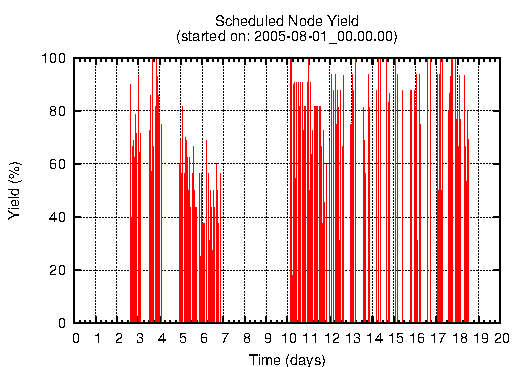
\includegraphics[width=\hsize]{./5-evaluation/figs/performance/yields/schNodeYield.pdf}
%% \end{center}
%% \caption{\small{\bf Scheduled node yield.}
%% {\em This graph shows the node yield out of the scheduled nodes for
%% each event.}}
%% \label{fig-schNodeYield}
%% \end{figure}

%% \begin{figure}[t]
%% \begin{center}
%% 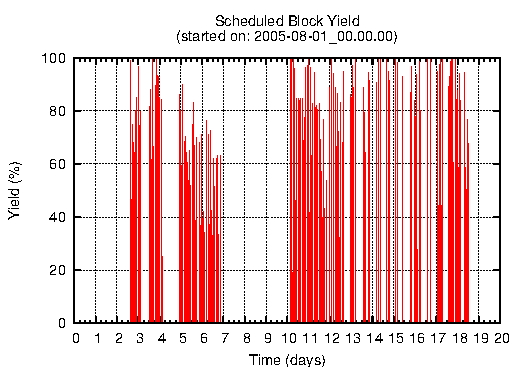
\includegraphics[width=\hsize]{./5-evaluation/figs/performance/yields/schBlockYield.pdf}
%% \end{center}
%% \caption{\small{\bf Scheduled block yield.}
%% {\em This graph shows the block yield out of the scheduled block for
%% each event.}}
%% \label{fig-schBlockYield}
%% \end{figure}

\subsection{Fetch latency}

Transfer latency directly impacts data yield. Because we disabled sampling on
each node (apart from node~250) during a Fetch download cycle, the duration
of the data transfer also affects a node's ability to record back-to-back
events.  

\begin{figure}[t]
\label{evaluation-fig-fetchlatency-byhops}
\begin{center}
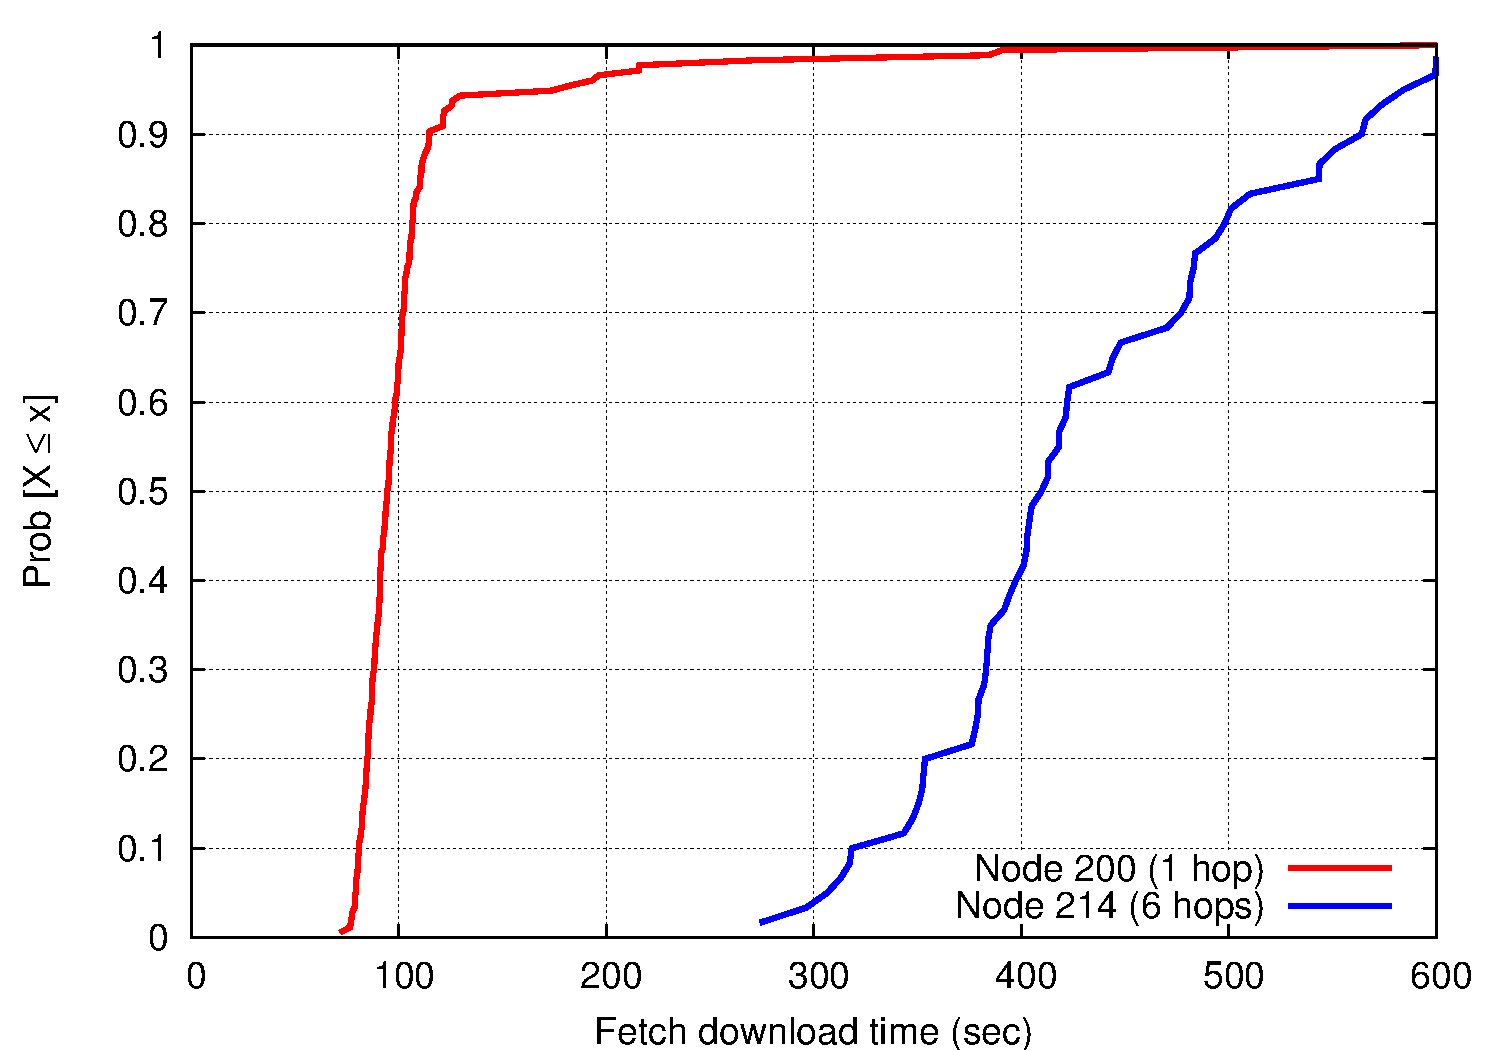
\includegraphics[width=\hsize]{./5-evaluation/figs/performance/CDFByHops/CDFBYHOPS.pdf}
\end{center}
\caption{\textbf{Distribution of Fetch latency for two nodes.}
The latency for a Fetch download depends on the depth of the node in the
routing tree, which affects both command propagation latency and reliability
of the routing path. Node~200 is located 1~hop from the sink and node~214 is
located 6~hops away.}
\end{figure}

The median latency for Fetch operations (downloading 60~sec worth of data
from a single node) was 186~sec and the 90th percentile was 444~sec.
Unsurprisingly, latency varies with the depth of the node in the routing
tree. Figure~\ref{evaluation-fig-fetchlatency-byhops} compares Fetch latency
for nodes 200~and~214, located 1~and~6 hops away from the sink, respectively.
Node~200 had a median Fetch latency of 94~sec, while node 214~had a median
latency of 409~sec, about 63~sec per hop.  This is due to both increased
delay for propagating Fetch command messages, as well as increasing packet
loss and retransmission overheads as the data flows over multiple hops to the
base.

%\begin{figure}[t]
%\begin{center}
%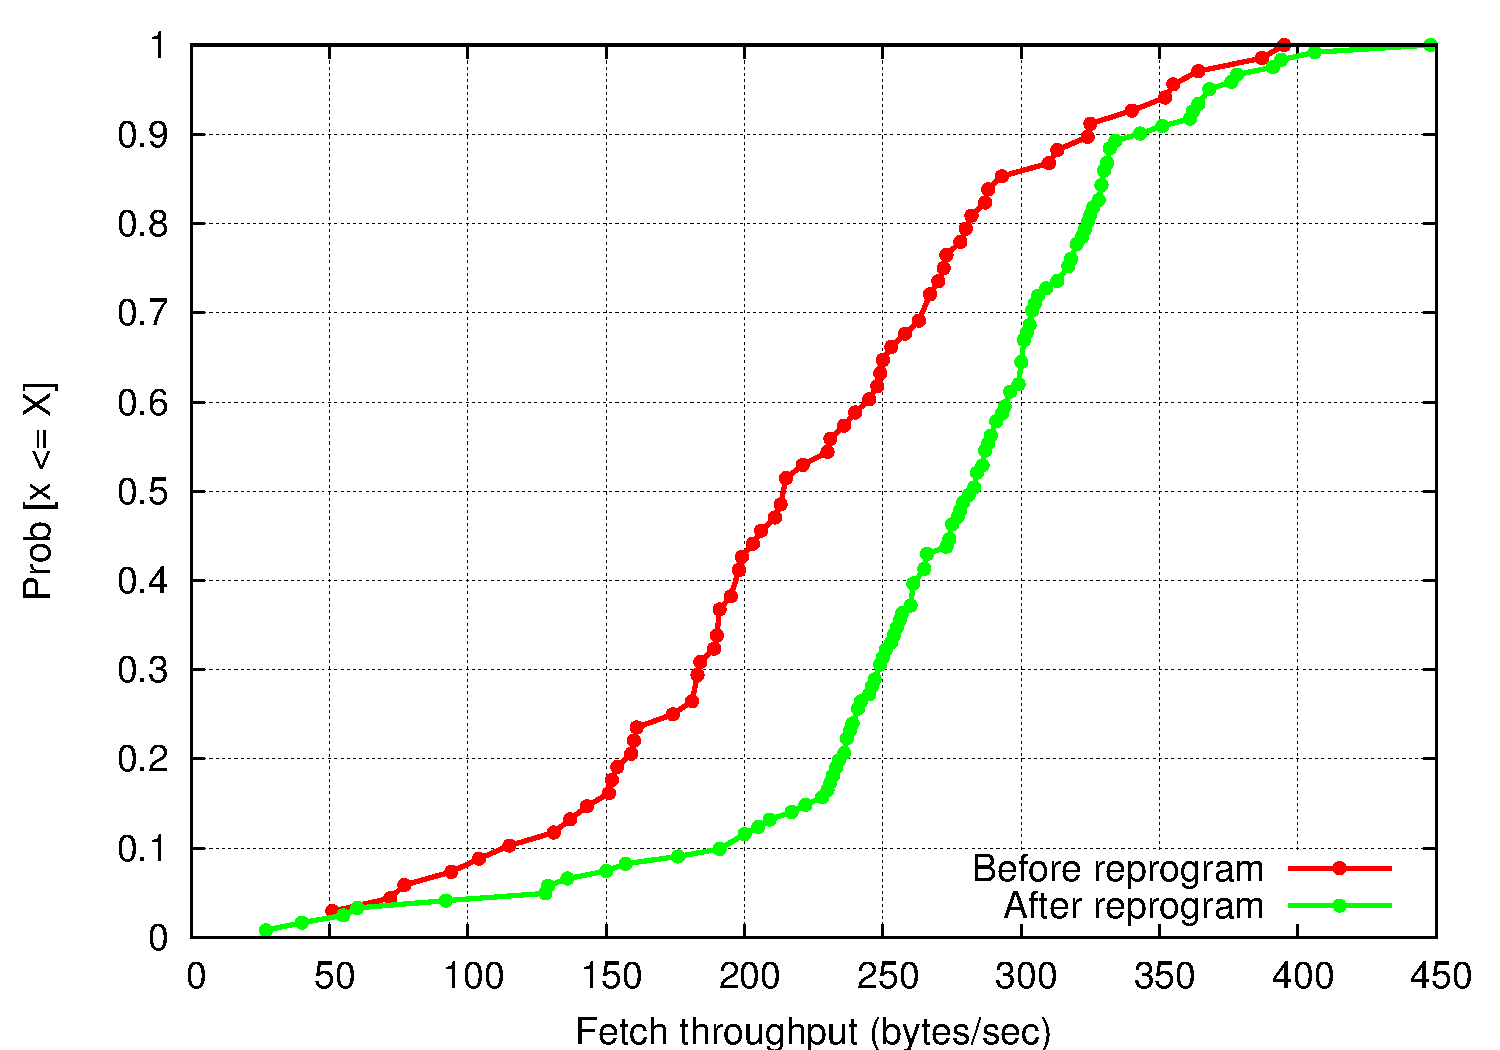
\includegraphics[width=\hsize]{./5-evaluation/figs/performance/fetchspeed/fetchspeed-cdf-oldnew.pdf}
%\end{center}
%\caption{\small{\bf Fetch throughput.}
%{\em This graph shows a CDF of the the throughput for each Fetch
%operation before and after the node reprogram. 
%Before programming, the median throughput was XXX~bytes/sec and after
%the median was~XXX~bytes/sec.}}
%\label{fig-fetchspeed-oldnew}
%\end{figure}

%Figure~\ref{fig-fetchspeed-oldnew} shows a CDF of the throughput of
%each Fetch operation from each node following an event. Before
%the network reprogram on August 11, the median throughput was
%215~bytes/sec; after the reprogram the median increased to 283~bytes/sec.
%While these values are far less than the peak thoughput achievable
%by the radio (which can exceed 12000 bytes/sec when MAC delays
%are accounted for), it is important to note that the Fetch protocol
%was never designed to maximize throughput. In particular, the 
%protocol requests a single block at a time from the network, and
%uses a long delay (up to 1~sec) before retransmitting a block request.

Fetch was initially designed to support reliable downloads of infrequent
events and we did not anticipate the need to capture back-to-back signals.
Unfortunately, these were common at Reventador, and may necessitate a
redesign. For example, it may be possible to reduce latency by streaming
multiple blocks in one request and reconstructing partial blocks after a
burst. Caching recently-received blocks on intermediate nodes could reduce
latency for repair requests~\cite{netshm-emnets05}.  However, such changes
would greatly increase the complexity of the protocol. For this deployment we
opted to prioritize simplicity and stability over performance.

%   - Throughput by hopcount
%\begin{figure}[t]
%\begin{center}
%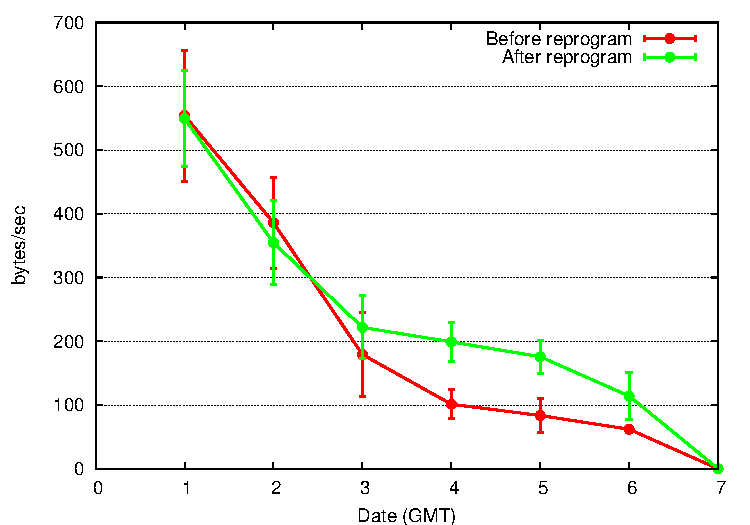
\includegraphics[width=\hsize]{./5-evaluation/figs/performance/fetchspeed-byhops/fetchspeed-oldnew.pdf}
%\end{center}
%\caption{\small{\bf Fetch throughput by node hop count.}
%{\em The throughput of fetch downloads diminishes rapidly as the
%hopcount distance to the node increases. This is due to increased
%packet loss and longer latencies for propagating fetch command
%messages. After reprogramming, fetch throughput increases primarily
%for nodes several hops from the base station.}}
%\label{fig-fetchspeed-byhops}
%\end{figure}

%  - Throughput [MDW]
%    - Bytes/sec
%\begin{figure}[t]
%\begin{center}
%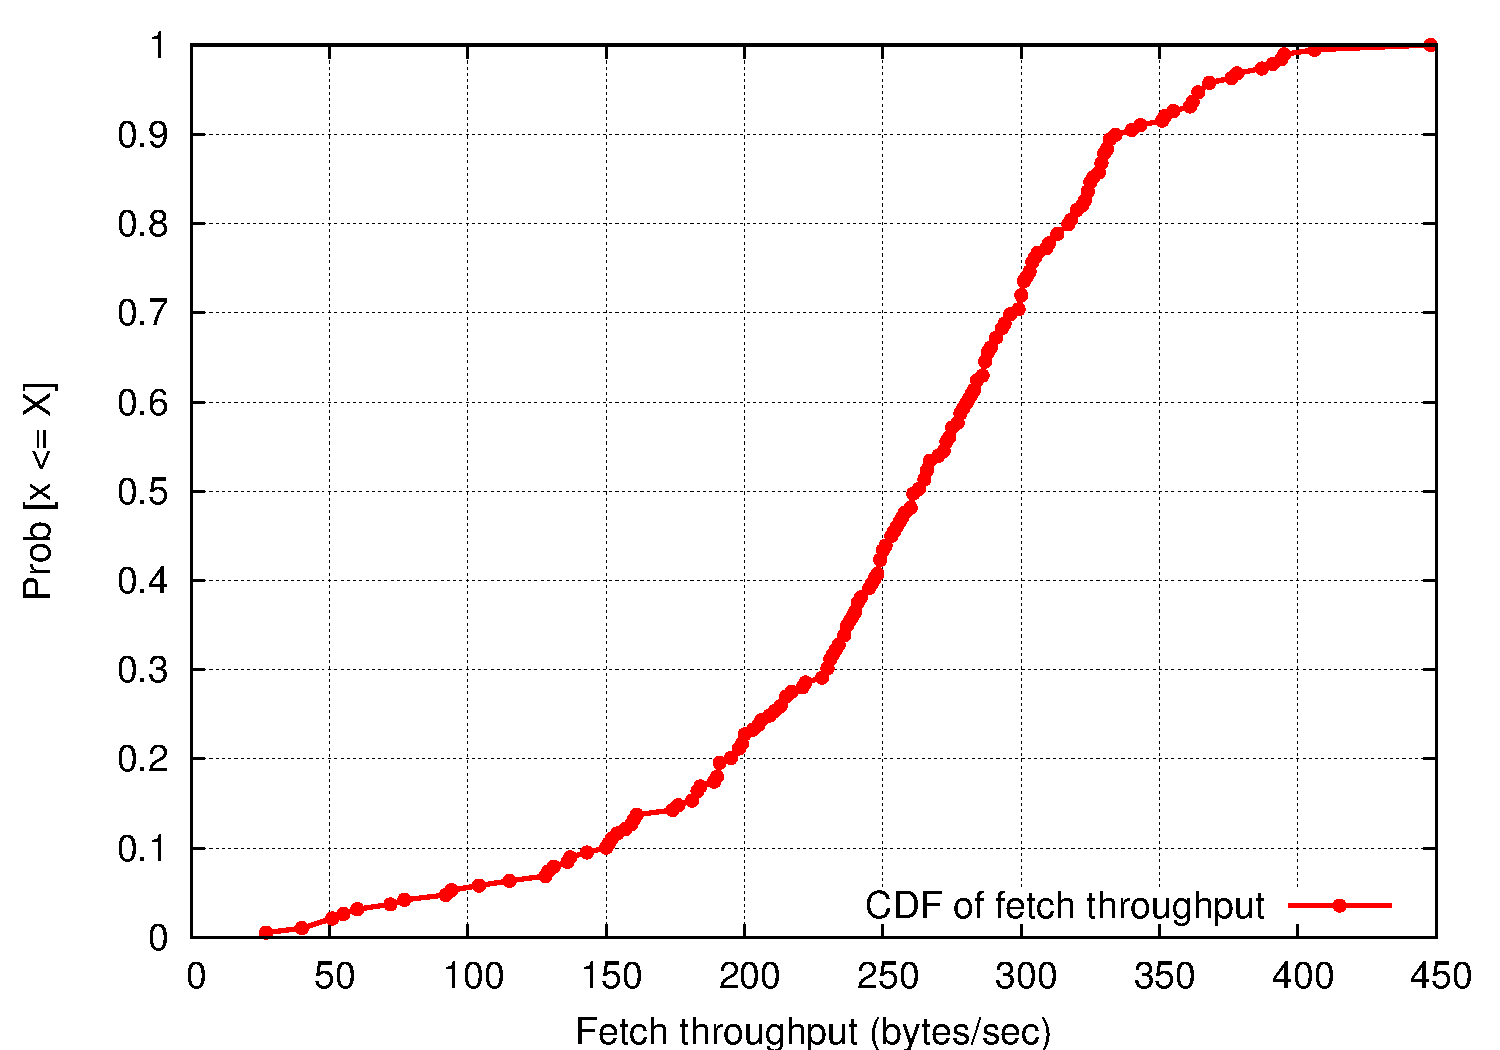
\includegraphics[width=\hsize]{./5-evaluation/figs/performance/fetchspeed/fetchspeed-cdf.pdf}
%\end{center}
%\caption{\small{\bf Fetch throughput.}
%{\em This graph shows a CDF of the the throughput for each fetch
%operation. The median throughput was XXX~bytes/sec and the
%mean~XXX~bytes/sec.}}
%\label{fig-fetchspeed}
%\end{figure}

% 23 Apr 2006 : GWA : Need to discuss this in text... TODO.

%    - Latency for data transfer
%\begin{figure}[t]
%\begin{center}
%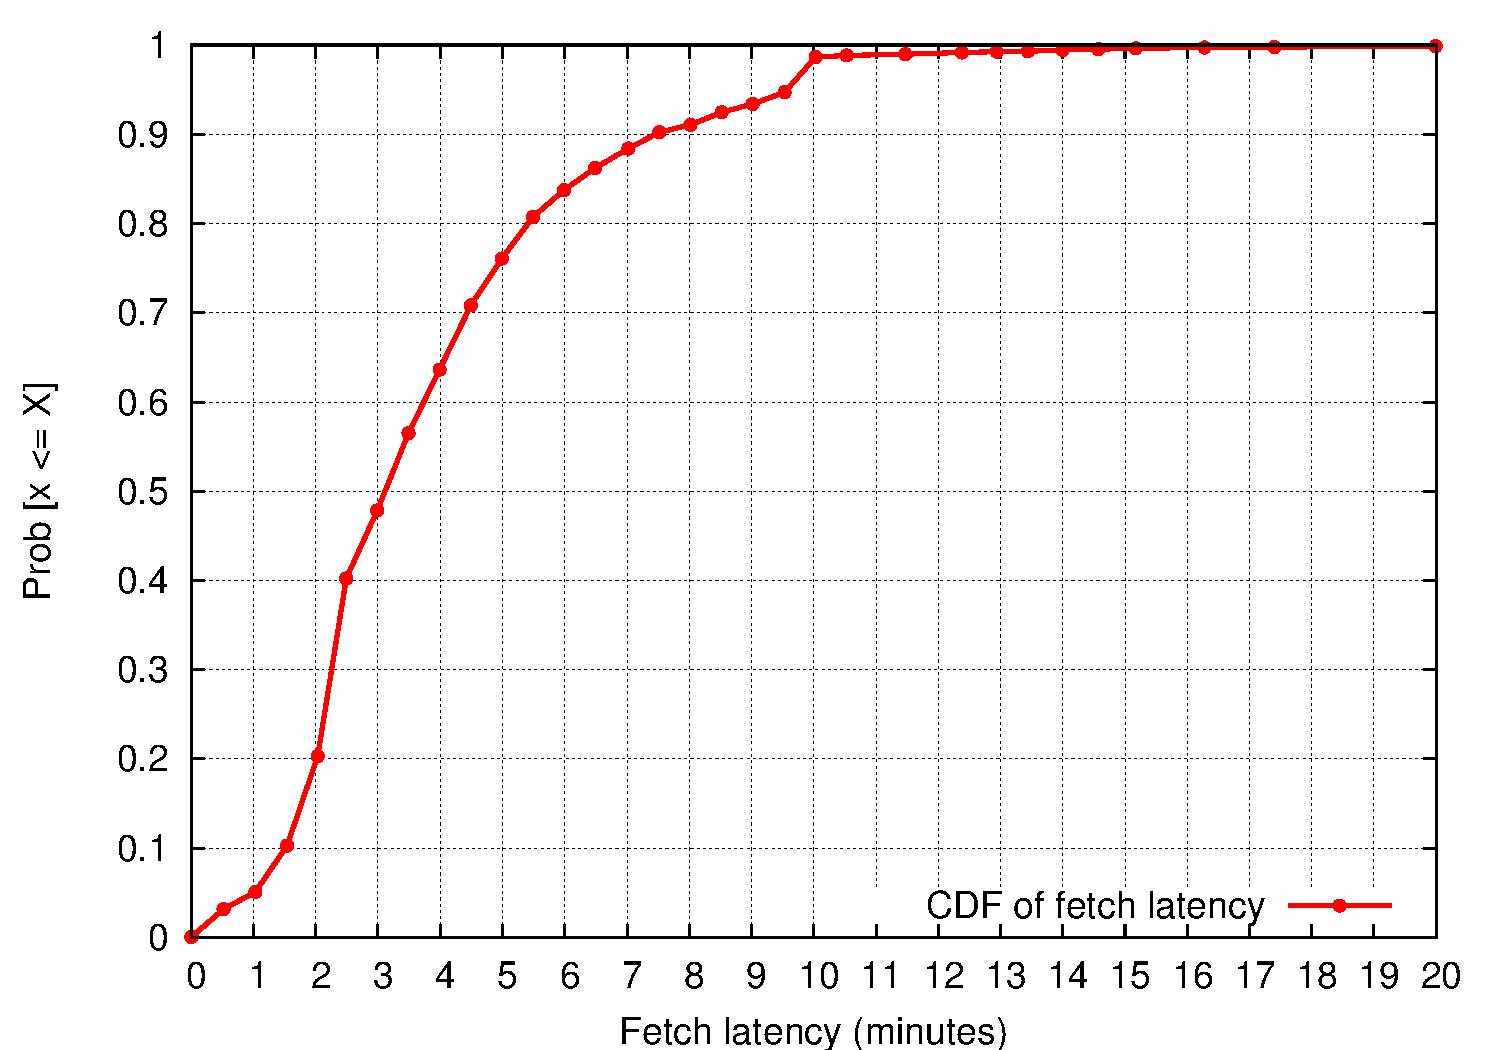
\includegraphics[width=\hsize]{./5-evaluation/figs/performance/fetchlatency/fetch-latency-cdf.pdf}
%\end{center}
%\caption{\small{\bf Fetch latency.}
%{\em This is a CDF of the latency for each fetch operation on a
%per-node basis. The median latency is just over 3~minutes, and the
%maximum latency (in all but a few cases) is 10~minutes.}}
%\label{fig-fetchlatency}
%\end{figure}

%    - Latency by hopcount
%\begin{figure}[t]
%\begin{center}
%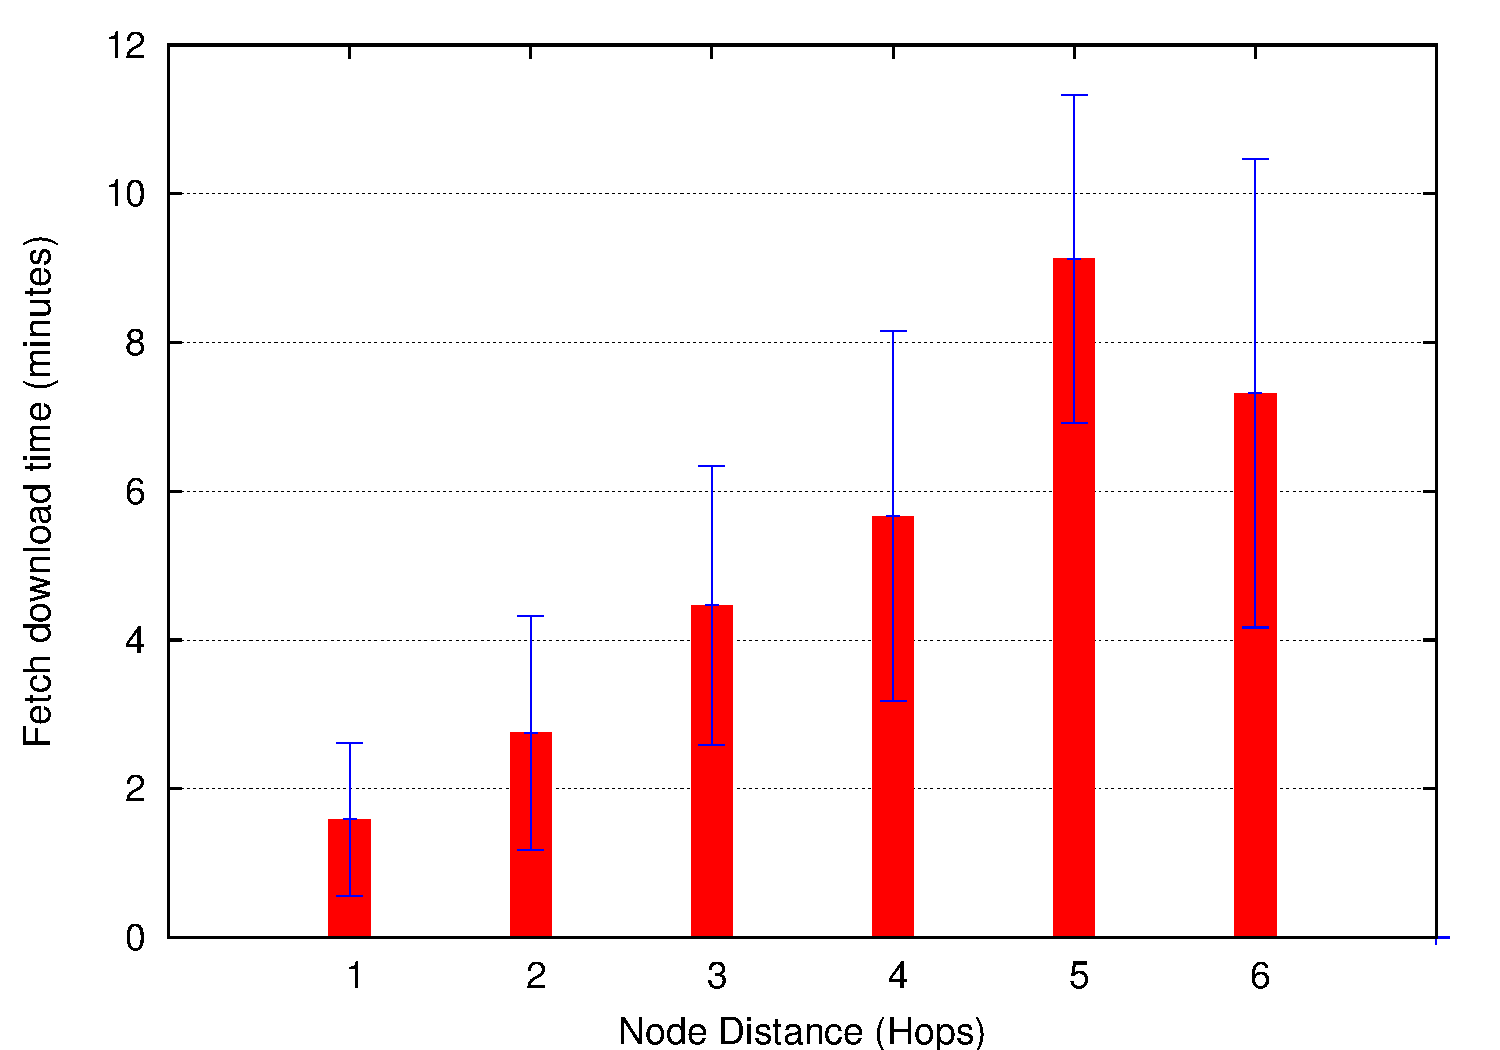
\includegraphics[width=\hsize]{./5-evaluation/figs/performance/fetchlatency/fetchlatency-byhops.pdf}
%\end{center}
%\caption{\small{\bf Fetch latency by hopcount.}
%{\em The latency for a Fetch download depends on the hop distance of
%the node from the root of the spanning tree, which affects both
%command propagation latency and reliability of the routing path.}}
%\label{fig-fetchlatency-byhops}
%\end{figure}


\section{Time Rectification and Accuracy}
\label{evaluation-sec-timing}

\begin{figure}[t!]
\begin{center}
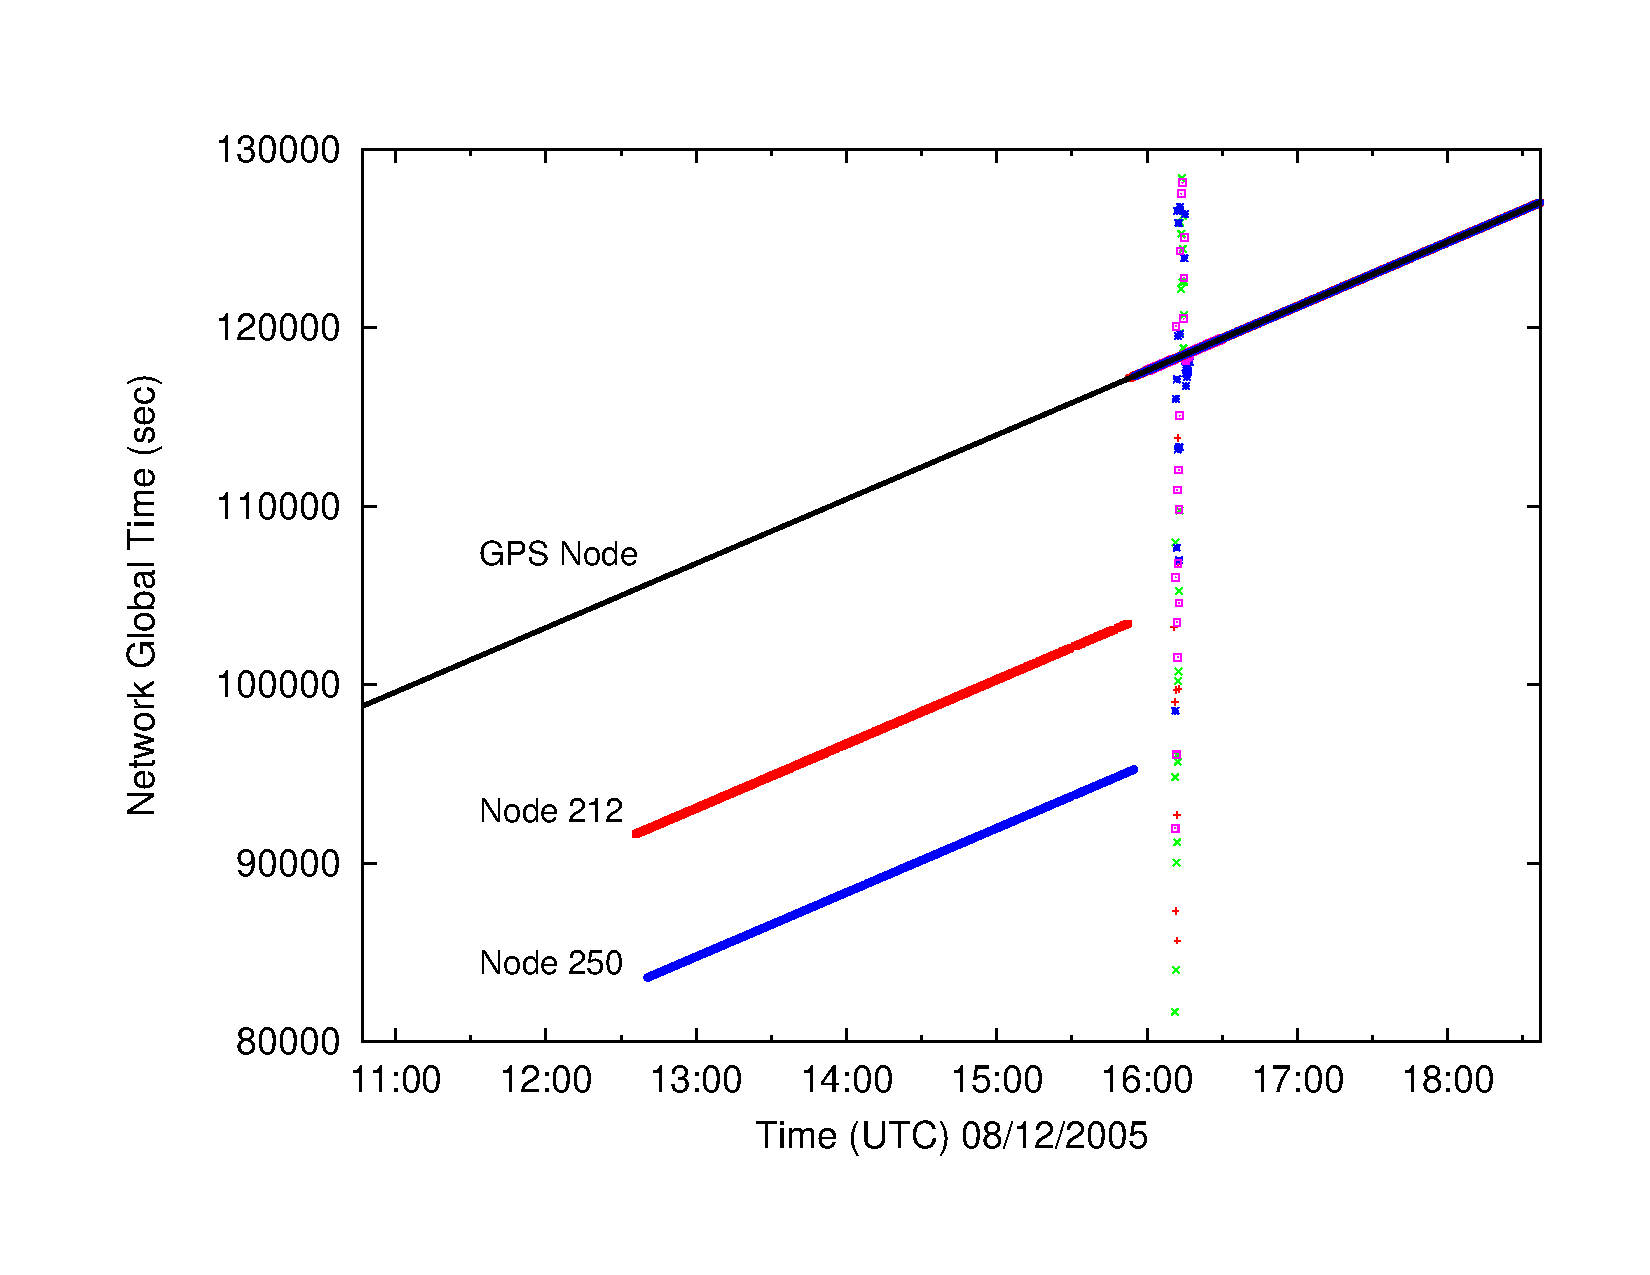
\includegraphics[width=\hsize]{./3-evaluation/figs/globaltimeproblem.pdf}
\end{center}

\caption{\textbf{Example of observed FTSP instability.} The global time value
reported by sensor nodes and the GPS node is plotted against the time that
the base station received the corresponding status messages. All nodes are
initially synchronized, but starting at 1230 GMT, Nodes~212 and 250 report
incorrect global times for the next 4.5~hours. When the nodes eventually
resynchronize, the global timestamps of other nodes initially experience some
instability.}

\label{evaluation-fig-globaltimeproblem}
\end{figure}

When analyzing seismoacoustic data acquired at volcanoes, accurate timing of
recorded signals is paramount. Studying volcanic source processes
necessitates precisely identifying the arrival time of P-~and S-waves at each
sensor, and correlating signals across the sensor array requires accurately
timestamping each sample.

Ideally, timing should be accurate to within one sample interval, or 10~ms
when sampling at 100~Hz. This requirement is an outgrowth of the prevalent
use of continuous wired data loggers within the seismological community,
which provide highly-accurate timestamps. Since these devices provide such
high-fidelity data, scientists within this community have not had to grapple
with the impacts of larger timing errors or sample reordering. It would be
interesting to discover how these kinds of errors would impact the end-to-end
process of seismological data analysis, but for the purposes of developing
trust in our initial collaboration we chose to try and match the capabilities
of existing instrumentation.

As described earlier, seismologists typically deploy a GPS receiver at each
station. Because GPS receivers are expensive and power hungry, we opted to
use a single GPS receiver and employ a multihop time-synchronization protocol
to establish a global timebase. The protocol worked well in laboratory
experiments. However, it experienced significant failures in the field,
requiring extensive postprocessing of the data to recover accurate timing for
each signal.

Prior internet measurement work has examined similar techniques for error
detection and recovery and produced valuable insights and
advice~\cite{paxson98calibrating,1028824} However, the specific techniques do
not map directly to our application for several reasons. First, they focus
more on error detection and do not address rectification. Second, the sensor
network time synchronization protocols we deployed are new and have goals
distinct from common network time-synchronization protocols. Additionally,
most network measurements can be performed using relative times only, whereas
the scientific requirements of our application required assigning an accurate
absolute timestamp to each collected sample.

In this section, we provide an overview of the time synchronization errors
observed in the field. We then present a novel \textit{time rectification}
technique that allows us to recover accurate timing despite protocol
failures. We evaluate our approach through lab experiments with a known,
ground-truth timebase and by comparing our signals with signals recorded by
the colocated data loggers.

\subsection{Time Synchronization Architecture}

We chose to use the Flooding Time Synchronization Protocol
(FTSP)~\cite{ftsp}, an existing protocol developed for wireless sensor nodes.
The original FTSP work reports timing errors of less than 67~$\mu$s for an
11-hop network of Mica2 nodes. We verified in our testbed that FTSP provided
a 90th-percentile time error of under 2.1~ms in a 5-hop linear network of
TMote Sky nodes.

FTSP works by using broadcast transmission and reception as a synchronous
moment that can identify the same time in two different frames: the sender's
and the receiver's\footnote{This ignores message propagation delay which,
given the speed of light, is taken to be neglible.}. FTSP uses the time kept
by a single node --- the FTSP root --- as the frame to which all other nodes
are synchronized. It uses special radio hooks to timetstamp outgoing messages
at the moment that they actually hit the air, which is typically different
from the time that the FTSP component sent them due to MAC delays. Incoming
messages are also timestamped at the moment of radio reception. By using
these two timestamps, one in the sender's frame of reference, the other in
the receiver's, a linear mapping from the sender's time to the receiver's can
be constructed. This mapping accounts for both time \textit{offset}
(resulting from nodes being booted or resetting their clocks at different
times) and \textit{skew}, differences in clock rates caused by oscillator
variation or environmental conditions. By performing a linear fit over only
the last several received timestamps, FTSP also accounts for \textit{drift},
slow changes in the oscillator rate over time. Each node participating in
FTSP periodically broadcasts messages allowing neighbors to construct a
timebase based on its own. This allows nodes multiple hops from the root node
to synchronize to the global timebase.

A single MicaZ sensor node was used as the root of the FTSP synchronization
tree. It interfaced to a Garmin GPS receiver and received a 1~Hz interrupt
synchronized to within 1~$\mu$s of the GPS ``pulse per second'' signal.
When the interrupt is raised, the node records the GPS time and corresponding
FTSP global time and sends a short message containing this information to the
base station. Each sensor node runs the FTSP protocol which maintains a
global timebase. Every 10~s, each node records its local time and the
corresponding FTSP global time, sending this information in its status
message to the base station. Finally, as each node records data, the first
sample of each block is marked with the node's local time. After downloading
data from each node following an event, this local time can be used to
recover the time for each sample in the block.

Therefore, we have three relevant timebases: the \textit{local time} at each
node; the \textit{global time} established by the FTSP protocol; and the
\textit{GPS time} recorded by the FTSP root. The information in the nodes'
status messages can be used to map local time to global time, and the
information in the GPS node's status messages can be used to map global time
to GPS-based GMT.

\subsection{FTSP Field Failures}
\label{evaluation-timing-deploymentfailures}

In the absence of failures, this mapping would be a straightforward process.
However, in the field, we noticed that nodes would occasionally lose
synchronization with the rest of the network and report FTSP global times
with significant errors, sometimes exceeding several hours. We suspect that
the sparse deployment conditions at the volcano might have led to different
behavior in the time synchronization protocol than in the lab. For example,
occasional message loss or failure of a neighbor could cause the node's
global time to drift from the rest of the network. However, in lab tests that
constrained the network topology we did not observe these instabilities.

Figure~\ref{evaluation-fig-globaltimeproblem} shows an example of the FTSP
instability observed in the field. The global time reported by two nodes
suddenly jumps off by several hours, and the nodes do not resynchronize until
rebooted 4.5~hours later. It turns out that two bugs conflated to cause this
problem. First, the TinyOS clock driver would occasionally return bogus local
timestamps. This bug was fixed in February 2006, several months after our
deployment. Second, FTSP does not check the validity of synchronization
messages, so a node reading an incorrect value for its local clock can
corrupt the state of other nodes, throwing off the global time calculation.

\begin{figure}[t]
\begin{center}
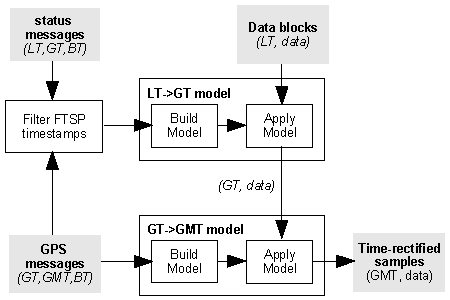
\includegraphics[width=0.8\hsize]{./3-evaluation/figs/rectificationcartoon.pdf}
\end{center}

\caption{\textbf{Time rectification process overview.}}

\label{evaluation-fig-rectificationcartoon}
\end{figure}

The failures of the time synchronization protocol make establishing the
correct GPS-based timestamp for each data sample extremely challenging. Our
\textit{time rectification} approach filters and remaps recorded timestamps
to accurately recover timing despite these failures. The time rectification
process is illustrated in Figure~\ref{evaluation-fig-rectificationcartoon}.
The first step is to \textit{filter} the global timestamps recorded by each
node, discarding bogus data. Second, we build a model mapping the local time
on each node to FTSP-based global time. Third, we use the GPS timestamp
information to build a second model mapping FTSP time to GMT. Finally, both
models are applied to the timestamps recorded in each data block producing a
GMT time for each sample.

\subsection{Timestamp Filtering}
\label{evaluation-subsection-filtering}

We begin by filtering out status messages appearing to contain incorrect
global timestamps. To do this, we correlate global timestamps from each node
against a common reference timebase and reject those that differ by more than
some threshold. For this, we use the base station laptop's local time, which
is \textit{only} used for filtering FTSP timestamps, not for establishing the
correct timing. The filtering process in is many ways similar to prior
work~\cite{paxson98calibrating,1028824} on detecting adjustments in
network-synchronized clocks.

We use the following abbreviations: \textit{LT} is the local time of a node;
\textit{GT} is the FTSP global time; \textit{BT} is the base station's local
time; and \textit{GMT} is the true GMT from the GPS signal. Each GPS status
message logged by the base station consists of the triple \textit{(GT, GMT,
BT)}. We use linear regression on this data to produce a reference timebase
mapping \textit{BT} to \textit{GT}.\footnote{We assume that the global time
reported by the GPS node is always correct; indeed, the definition of
``global time'' is the FTSP time reported by the GPS node. We verified that
the FTSP instability affecting the sensor nodes did not occur on the GPS
node, most likely because the MicaZ uses a different processor that is
unaffected by the clock driver bug.} For each node status message logged by
the laptop \textit{(LT, GT, BT)}, we map \textit{BT} to the expected
$\mathit{GT}_{\mathit{ref}}$ using the reference timebase. If $ \mid
\mathit{GT}_{\mathit{ref}} - \mathit{GT} \mid > \delta$, we discard the
status message from further consideration. We use a threshold of $\delta =
1$~s. Although radio message propagation and delays on the base station can
affect the \textit{BT} for each status message, a small rejection threshold
$\delta$ makes it unlikely that any truly incorrect FTSP timestamps pass the
filter. Indeed, of the 7.8\% of timestamps filtered out, the median
\textit{GT} error was 8.1~hours.
Figure~\ref{evaluation-fig-rectificationexample} shows an example of errant
timestamps being removed.


\subsection{Timestamp Rectification}
\label{evaluation-subsec-timerectification}

\begin{figure}[t]
\begin{center}
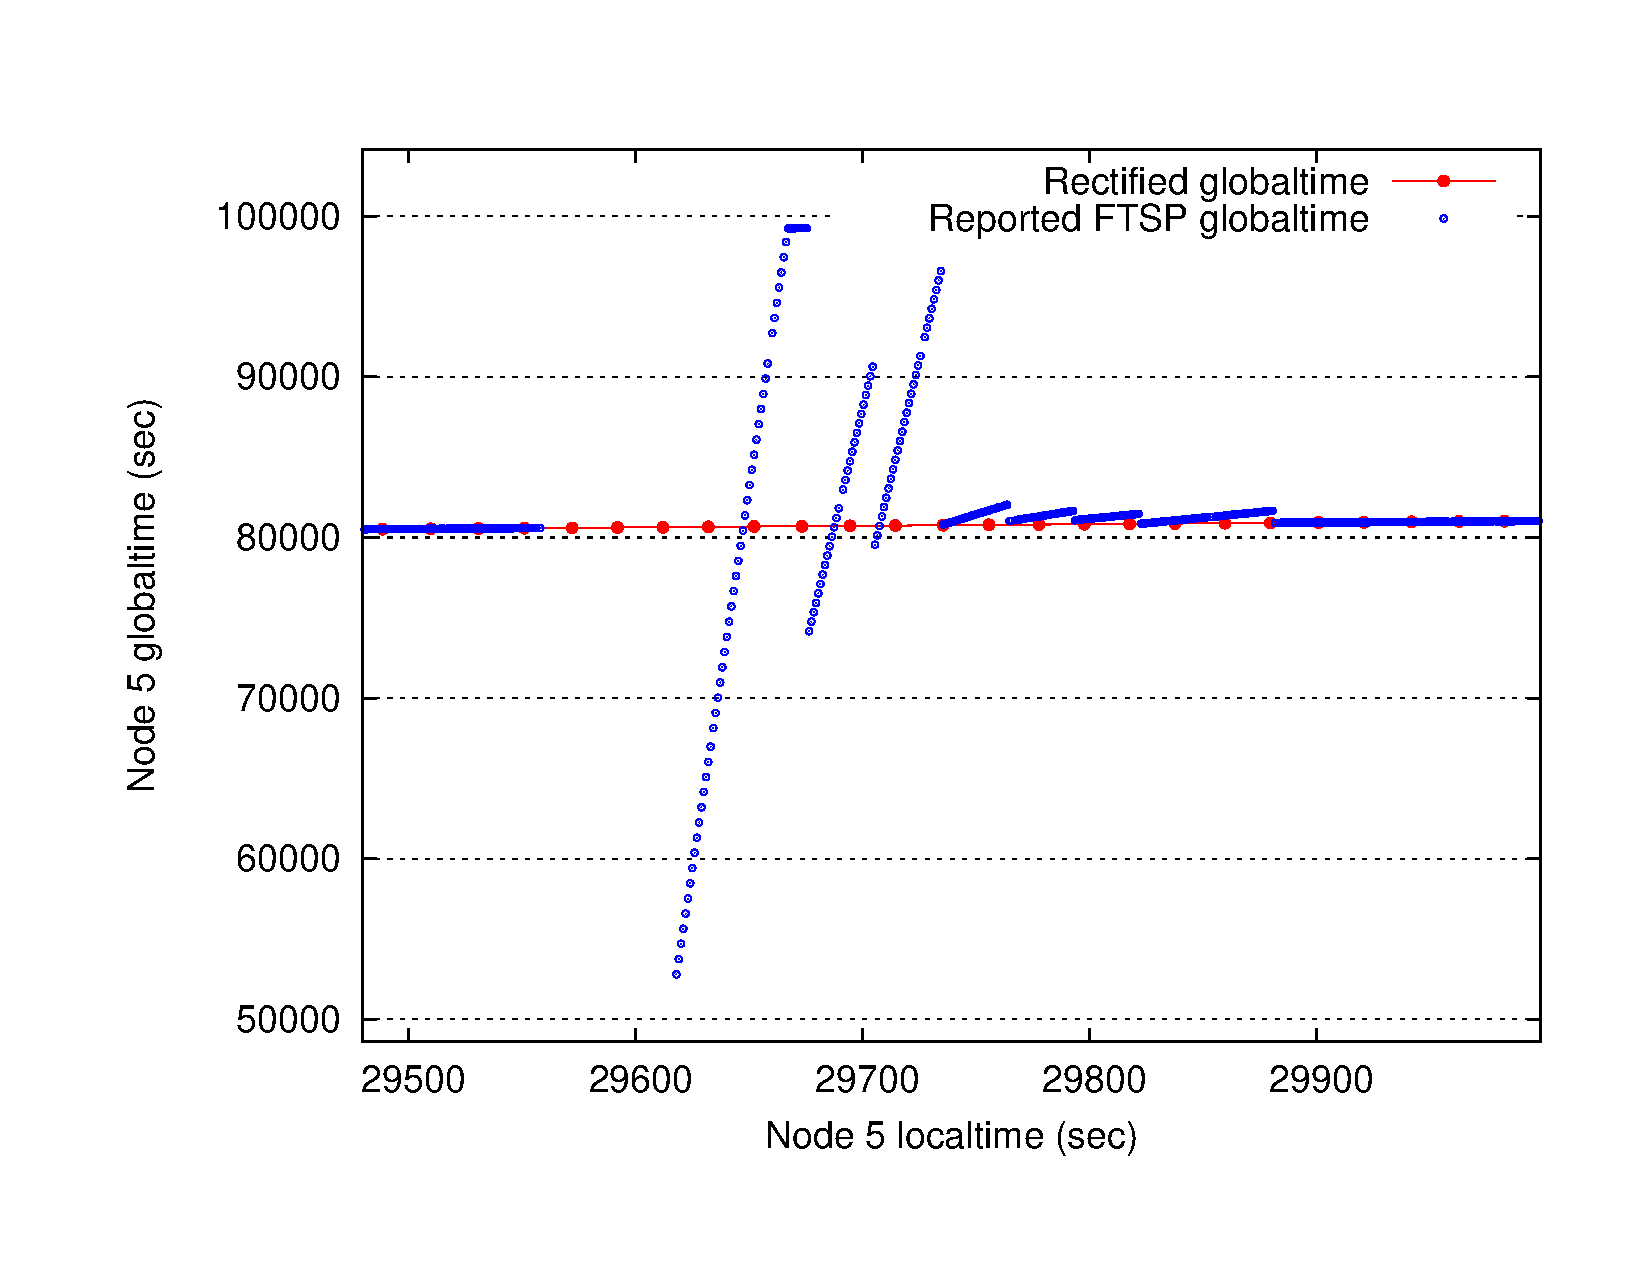
\includegraphics[width=\hsize]{./3-evaluation/figs/rectificationexample.pdf}
\end{center}

\caption{\textbf{Time rectification example.} The raw (LT, GT) pairs
collected from the node show that it experiences a period of FTSP
instability. The time rectification process removes the errant timestamps
creating an accurate mapping between LT and GT created using a linear
regression on the remaining timestamps.}

\label{evaluation-fig-rectificationexample}
\end{figure}

The goal of \textit{time rectification} is to assign a GMT timestamp to each
sample in the recorded data. In order to do so, we build two models: one
mapping a node's local time to global time, and another mapping global time
to GMT.

From those status messages that pass the filter, we build a piecewise linear
model mapping \textit{LT} to \textit{GT} using a series of linear
regressions. We construct separate models for each node, since local times
vary significantly between nodes. Each regression spans up to 5~minutes of
data and we initiate a new regression if the gap between subsequent
\textit{(LT, GT)} pairs exceeds 5~minutes. Each interval must contain at
least two valid status messages to construct the model. We take the
\textit{LT} value stored in each data block and use this model to recover the
corresponding \textit{GT} value.

The next step is to map global time to GMT. Each of the GPS node's status
messages contain a \textit{(GT, GMT)} pair. As above, we build a piecewise
linear model mapping \textit{GT} to \textit{GMT}, and apply this model to the
\textit{GT} values for each data block. Finally, we assign a GMT value to
each sample contained in the block, using linear interpolation between the
GMT values assigned to the first sample in each block. This process makes no
assumptions about sampling rate, which varies slightly from node to node due
to clock drift.

\subsection{Evaluation}
\label{evaluation-timing-postdeployment}

Evaluating this time rectification process has proved difficult, primarily
because we have no ground truth for the timing of the signals recorded in the
field. However, by reproducing the deployment conditions in the lab, we were
able to measure the accuracy of the recovered timing in a controlled setting.
In addition, as described earlier, two GPS-synchronized data loggers were
colocated with our sensor network, providing us the opportunity to directly
compare our time-rectified signals with those recorded by conventional
instrumentation.

Our first validation took place in the lab. Feeding the output of a signal
generator to both a miniature version of our sensor network and to a
Reftek~130 data logger allowed us to directly compare the data between both
systems. The miniature network consisted of a single sensor node, routing
gateway, and GPS receiver node. The same software was used as in the field
deployment. The Reftek~130 logs data to a flash memory card and timestamps
each sample using its own GPS receiver. The Reftek~130 is commonly used in
volcano field studies and its timing accuracy has been extensively validated.

The results showed a consistent 15~ms offset between the time-rectified
signals recorded by the sensor node and the Reftek data logger. We discovered
that this offset was due to delays introduced by the digital filtering
performed by the ADC on our sensor board. Adjusting for this delay resulted
in an indiscernible offset between the sensor node and Reftek signals. While
this experiment does not reproduce the full complexity of our deployed
network, it does serve as a baseline for validation.

In the second lab experiment, we set up a network of 7~sensor nodes in a
6-hop linear topology. The topology is enforced by software, but all nodes
are within radio range of each other, making it possible to stimulate all
nodes simultaneously with a radio message. Each node samples data and sends
status messages using the same software as the field deployment. The FTSP
root node periodically transmits a beacon message. On reception of the
beacon, each node records the FTSP global timestamp of the message reception
time (note that reception of the beacon message is not limited by the
software-induced topology). Because we expect all nodes to receive this
message at the same instant, modulo interrupt latency jitter, we expect the
FTSP time recorded by each node to be nearly identical. The FTSP root also
records the time that the beacon was transmitted, accounting for MAC delay.
The experiment ran for 34~hours, during which time FTSP experienced
instabilities similar to those seen during our deployment.

\begin{table}[t]
\begin{center}
\begin{tabular}{|lll|} \hline & \textbf{Raw error} & \textbf{Rectified error} \\ \hline
\textbf{1 hop}, 50th percentile & 1.52 ms & 1.42 ms \\
\textbf{1 hop}, 90th percentile & 9.86 ms & 6.77 ms \\ \hline
\textbf{6 hops}, 50th percentile & 2.63 ms & 2.18 ms \\
\textbf{6 hops}, 90th percentile & 13.5 ms & 6.8 ms \\ \hline
\end{tabular}
\end{center}

\caption{\textbf{Timestamp errors in a 6-hop lab testbed.} This table shows
the 50th and 90th-percentile timing errors on both the raw FTSP timestamps,
and rectified timestamps.}

\label{evaluation-fig-time-rect-lab}
\end{table}

This allows us to compare the \textit{true} global time of each beacon
message transmission and the \textit{apparent} global time on each receiving
node, both before and after subjecting the data to our time rectification
process. We call the difference between the true and apparent times the
\textit{timestamp error}. Figure~\ref{evaluation-fig-time-rect-lab} shows the
results for nodes one and six hops away from the FTSP root. After
rectification, 99.9\% of the errors for the one-hop node and 93.1\% of the
errors for the six-hop node fall within our 10~ms error envelope.

\subsection{Comparison with Broadband Station}
\label{evaluation-sec-datagroundtruthing}

\begin{figure}[t]
\begin{center}
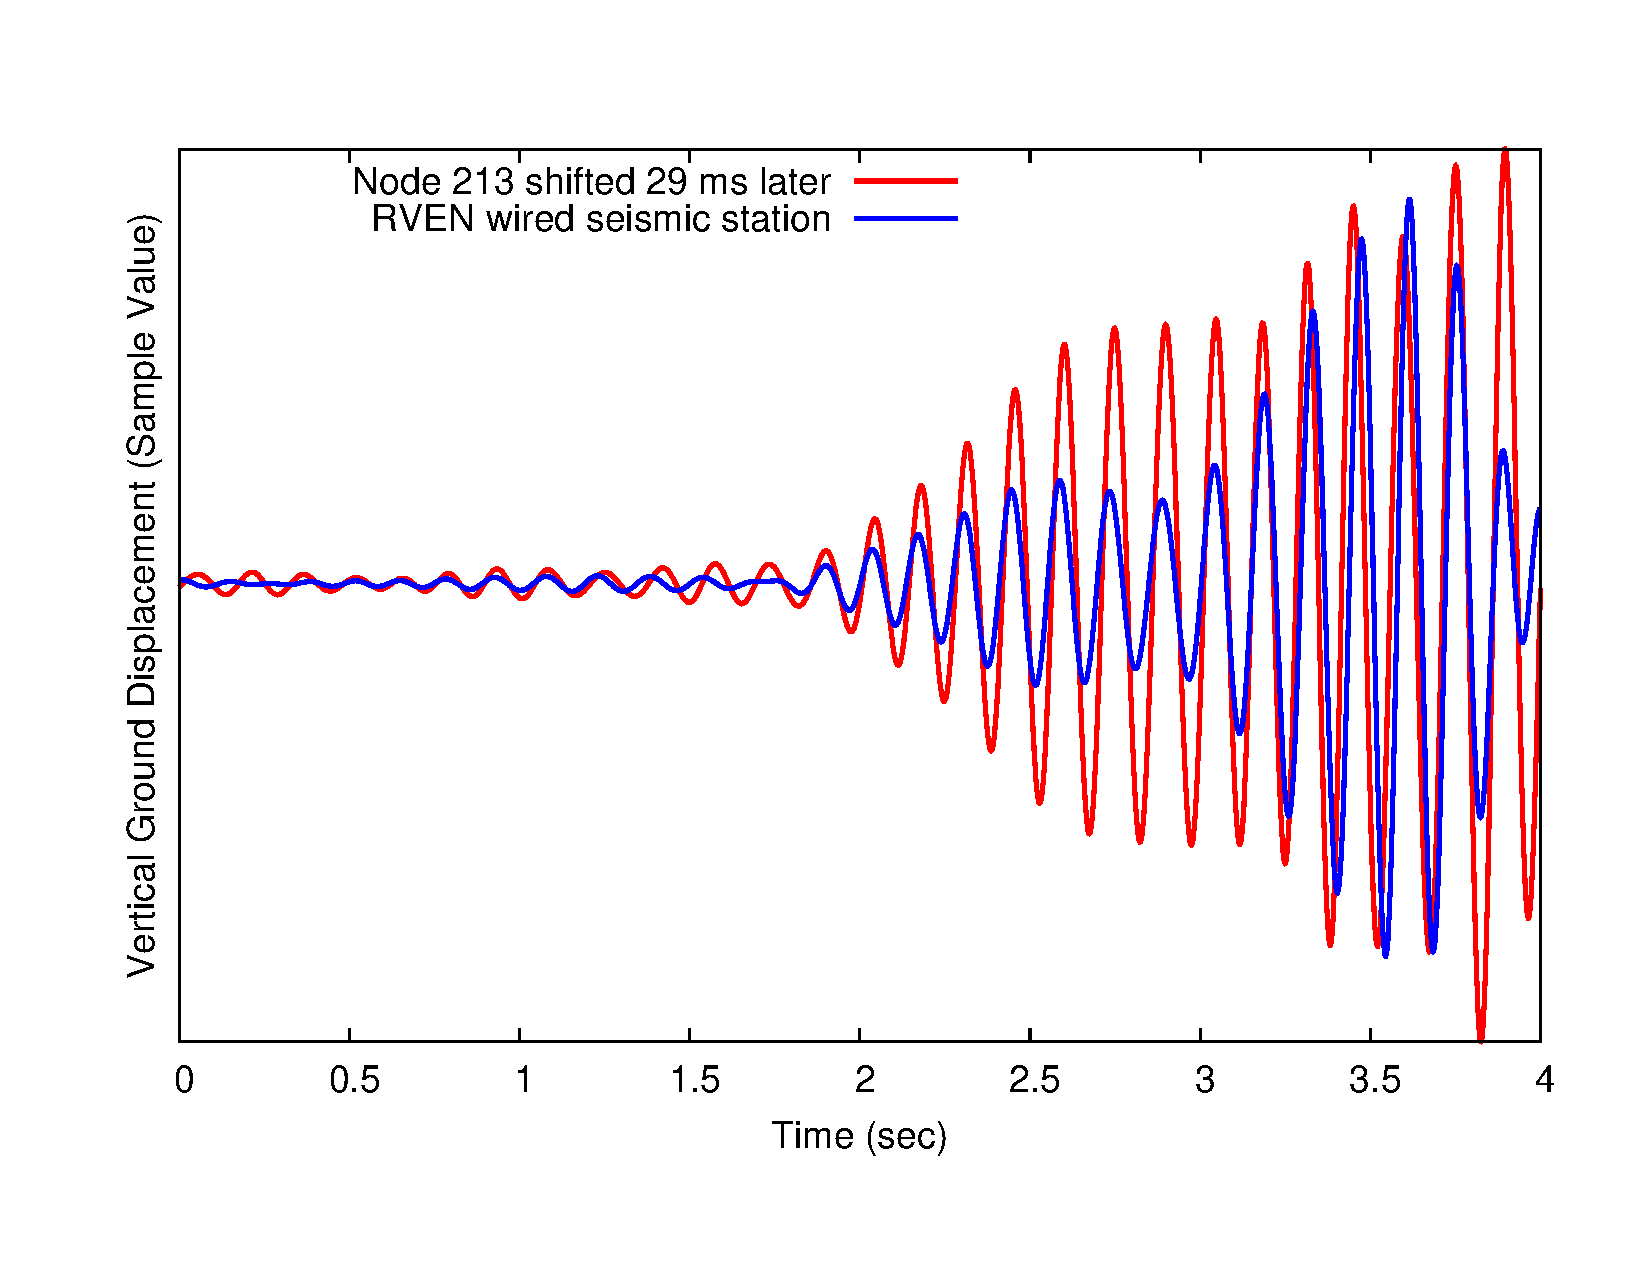
\includegraphics[width=\hsize]{./3-evaluation/figs/broadbandmatch.pdf}
\end{center}

\caption{\textbf{Comparison of RVEN and Node~213 signals.} This figure shows
two seismic waves recorded by sensor node 213 and a broadband seismometer
located 56~m away. After time rectification, a 29~ms time shift produces an
excellent match.}

\label{evaluation-fig-broadbandmatch}
\end{figure}

\begin{figure}[t]
\begin{center}
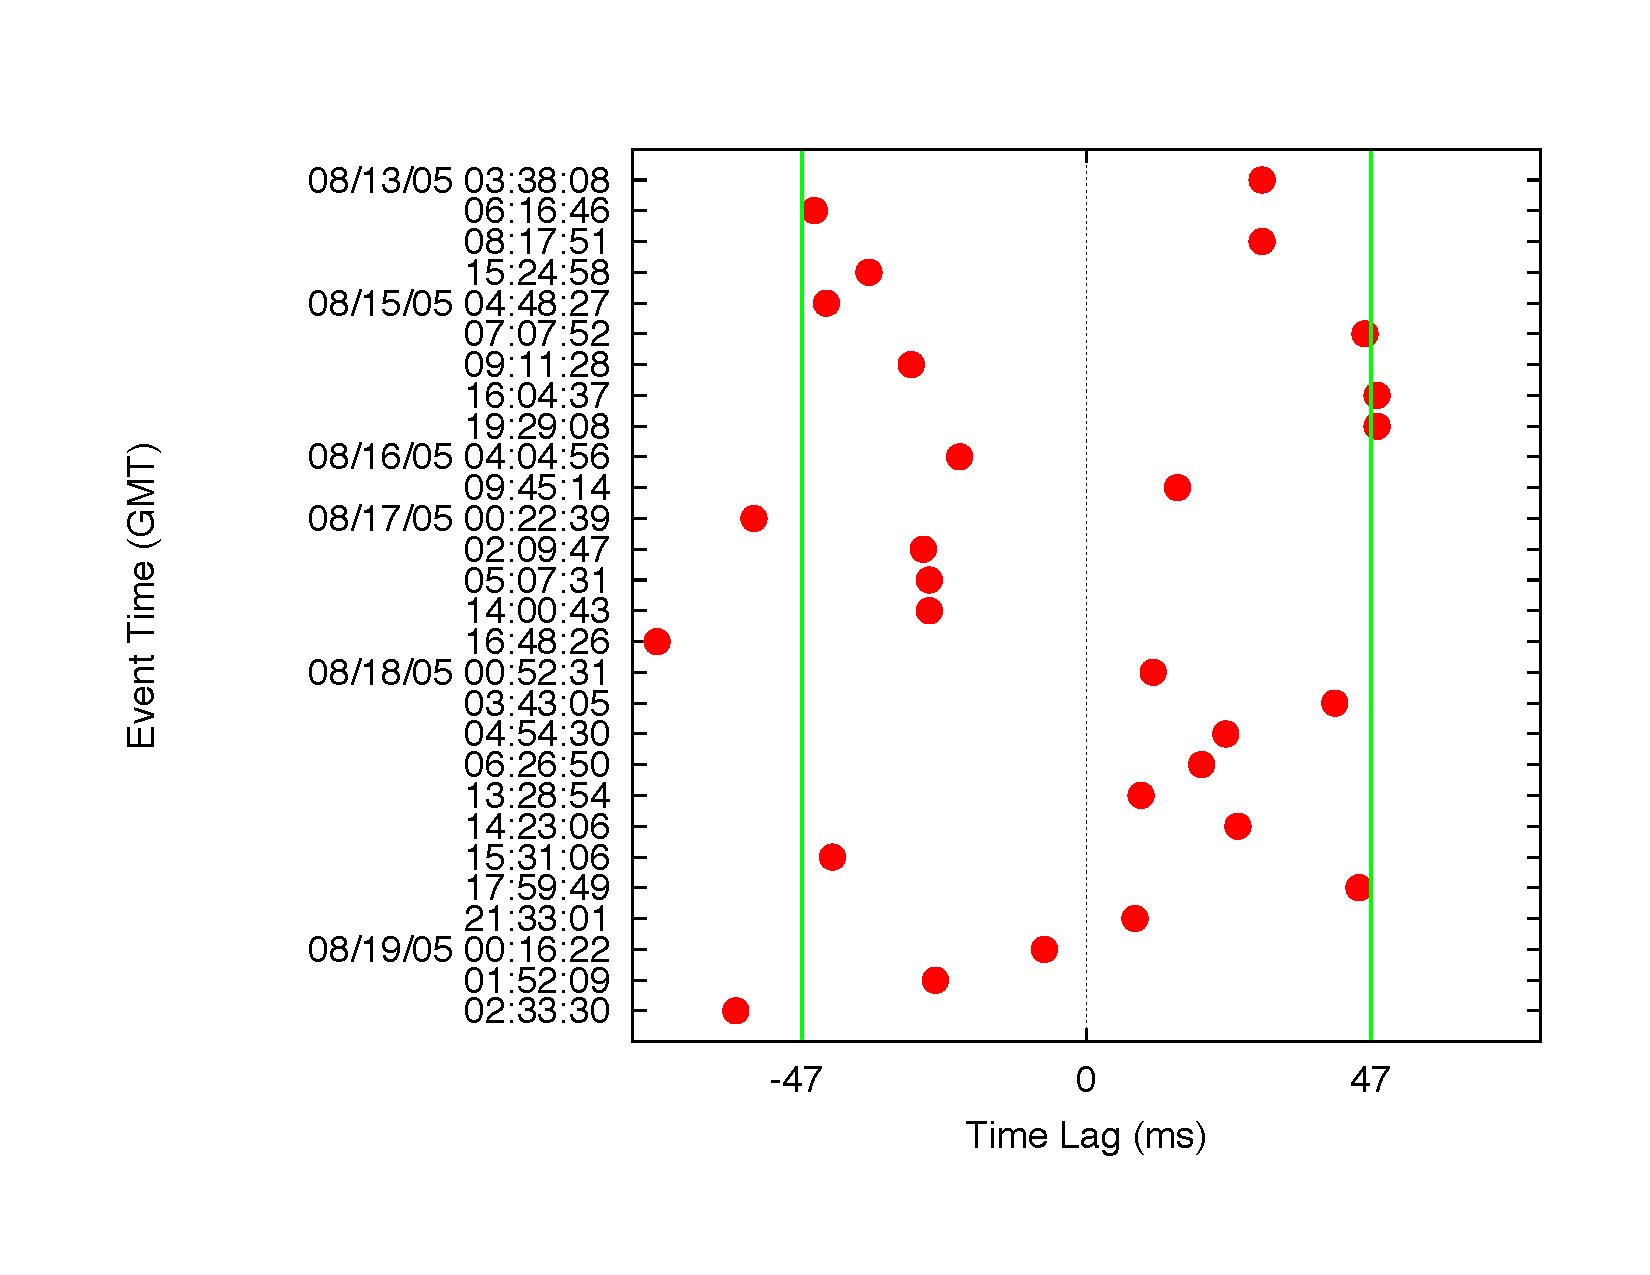
\includegraphics[width=\hsize]{./3-evaluation/figs/timingscatterplot.pdf}
\end{center}

\caption{\textbf{Lag times between Node~213 and RVEN.} The best lag time
between the two stations is shown for 28 events. Most time shifts fall into
the +/-~47~ms window that we would expect given the distance between the two
stations and up to 10~ms of timing error.}

\label{evaluation-fig-timingscatterplot}
\end{figure}


Although time rectification works well in the laboratory, it is also
necessary to evaluate its accuracy on the data collected during the field
deployment. For this purpose, we made use of one of the broadband seismometer
stations colocated with our sensor network. The RVEN (for ``Reventador
vent'') station was located 56~m from sensor Node~213. Given their proximity,
we would expect the seismic waveforms captured by both RVEN and Node~213 to
be well correlated. Some time shift between the two signals would be
expected: a seismic wave passing each station could be as slow as 1.5~km/sec,
so the time lag between the signals could be as high as 37~ms. However, due
to differences in the seismometers and the placement and ground coupling of
the sensors, we would not expect perfectly correlated signals in every case.

We identified 28~events recorded by both RVEN and Node~213. The data for
Node~213 was time rectified as described earlier, and the RVEN data was
timestamped by the Reftek's internal GPS receiver. We applied a bandpass
filter of 6--8~Hz to each signal to reduce sensor-specific artifacts. The
cross-correlation between the signals produces a set of of \textit{lag times}
indicating possible time shifts between the two signals. Due to the periodic
nature of the signals, this results in several lag times at multiples of the
dominant signal period. For each lag time, we visually inspected how well the
time-shifted signals overlapped and picked the best match by hand.

Figure~\ref{evaluation-fig-broadbandmatch} shows an example of this process
that demonstrates excellent correlation between the RVEN and Node~213 signals
with a 29~ms time shift. Figure~\ref{evaluation-fig-timingscatterplot} shows
a scatterplot of the best lag times for all~28~events. Of these, only
5~events fall outside of a $+/-$~47~ms window defined by the distance between
the stations ($+/-$~37~ms) and our acceptable sampling error (10~ms). We have
high confidence that our time rectification process was able to recover
accurate timing despite failures of the FTSP protocol.

\section{Data Fidelity}
\label{evaluation-sec-fidelity}

The final and most important measure of our network is its ability to provide
scientifically-meaningful data on the volcano's activity. In this section, we
perform an initial analysis of the seismic and acoustic signals from a
seismological perspective, with the goal of validating the accuracy of the
signal quality and timing.

\subsection{Acoustic wave propagation}

The infrasonic (low-frequency acoustic) waves generated by the volcano are
primarily the result of explosive events. 
%% As such, infrasound is a useful complement to seismic monitoring and
%% can be used to differentiate explosions from other kinds of
%% earthquakes.
We start by measuring the velocity of infrasonic waves recorded by our
network, which is more straightforward than seismic analysis for several
reasons.  First, infrasonic waves generate a clear impulse in the microphone
signal, making it easy to determine the time of the wave arrival at each
sensor. In addition, acoustic waves propagate about an order of magnitude
slower than seismic waves (roughly 340~m/s versus 1500-4000~m/s).
%% , and compared to ground-propagating seismic waves, air is a
%% relatively homogenous medium.
We also expect an infrasonic wave to originate at the vent of the volcano,
simplifying the wave velocity calculation.

%% \begin{figure*}[t]
%% \begin{center}
%% \begin{tabular}{cc}
%% 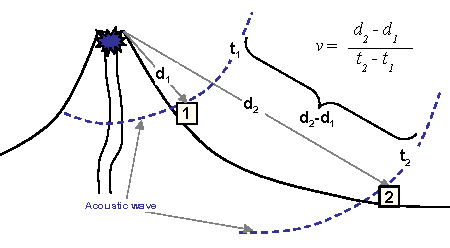
\includegraphics[width=0.4\hsize]{./5-evaluation/figs/fidelity/acousticSeismicSketches.pdf}
%% &
%% 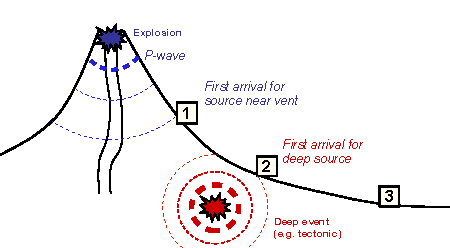
\includegraphics[width=0.4\hsize]{./5-evaluation/figs/fidelity/acousticSeismicSketches2.pdf}
%% \\
%% {\small\bf (a) Acoustic wave propagation} &
%% {\small\bf (b) Seismic wave propagation} \\
%% \end{tabular}
%% \end{center} 
%% \caption{\small {\bf Computing wave arrivals of seismic and acoustic
%% waves.} {\em These sketches show the propagation of (a) acoustic
%% and (b) seismic waves from the volcano. While acoustic waves emanate
%% from the vent, seismic waves may be generated by explosions from the
%% vent or sources within the volcano.}}
%% \label{fig-acousticSketch}
%% \label{fig-seismicSketch}
%% \end{figure*}

\begin{figure}[t]
\label{evaluation-fig-acousticSketch}
\begin{center}
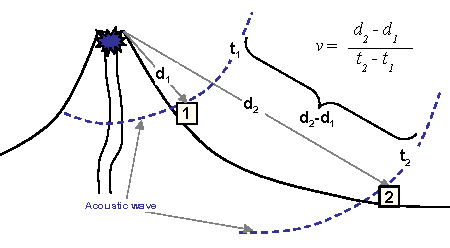
\includegraphics[width=\hsize]{./5-evaluation/figs/fidelity/acousticSeismicSketches.pdf}
\end{center}
\caption{\textbf{Computing acoustic wave velocity.}
The velocity of the acoustic wave is calculated based on the distance of each
station from the vent, $d_i$, and the arrival time of the wave at each
station, $t_i$.}
\end{figure}

We identified four events in our data set with a clear infrasonic component.
For each event, we hand-picked the arrival time of the wave at each node
using the time-rectified signal.  Figure~\ref{evaluation-fig-acousticArrival}
plots the wave arrival time versus the distance of each node from the vent.
As shown in Figure~\ref{evaluation-fig-acousticSketch}, the velocity of the
wave can be calculated by performing a linear regression on this dataset.

\begin{figure}[t]
\label{evaluation-fig-acousticArrival}
\begin{center}
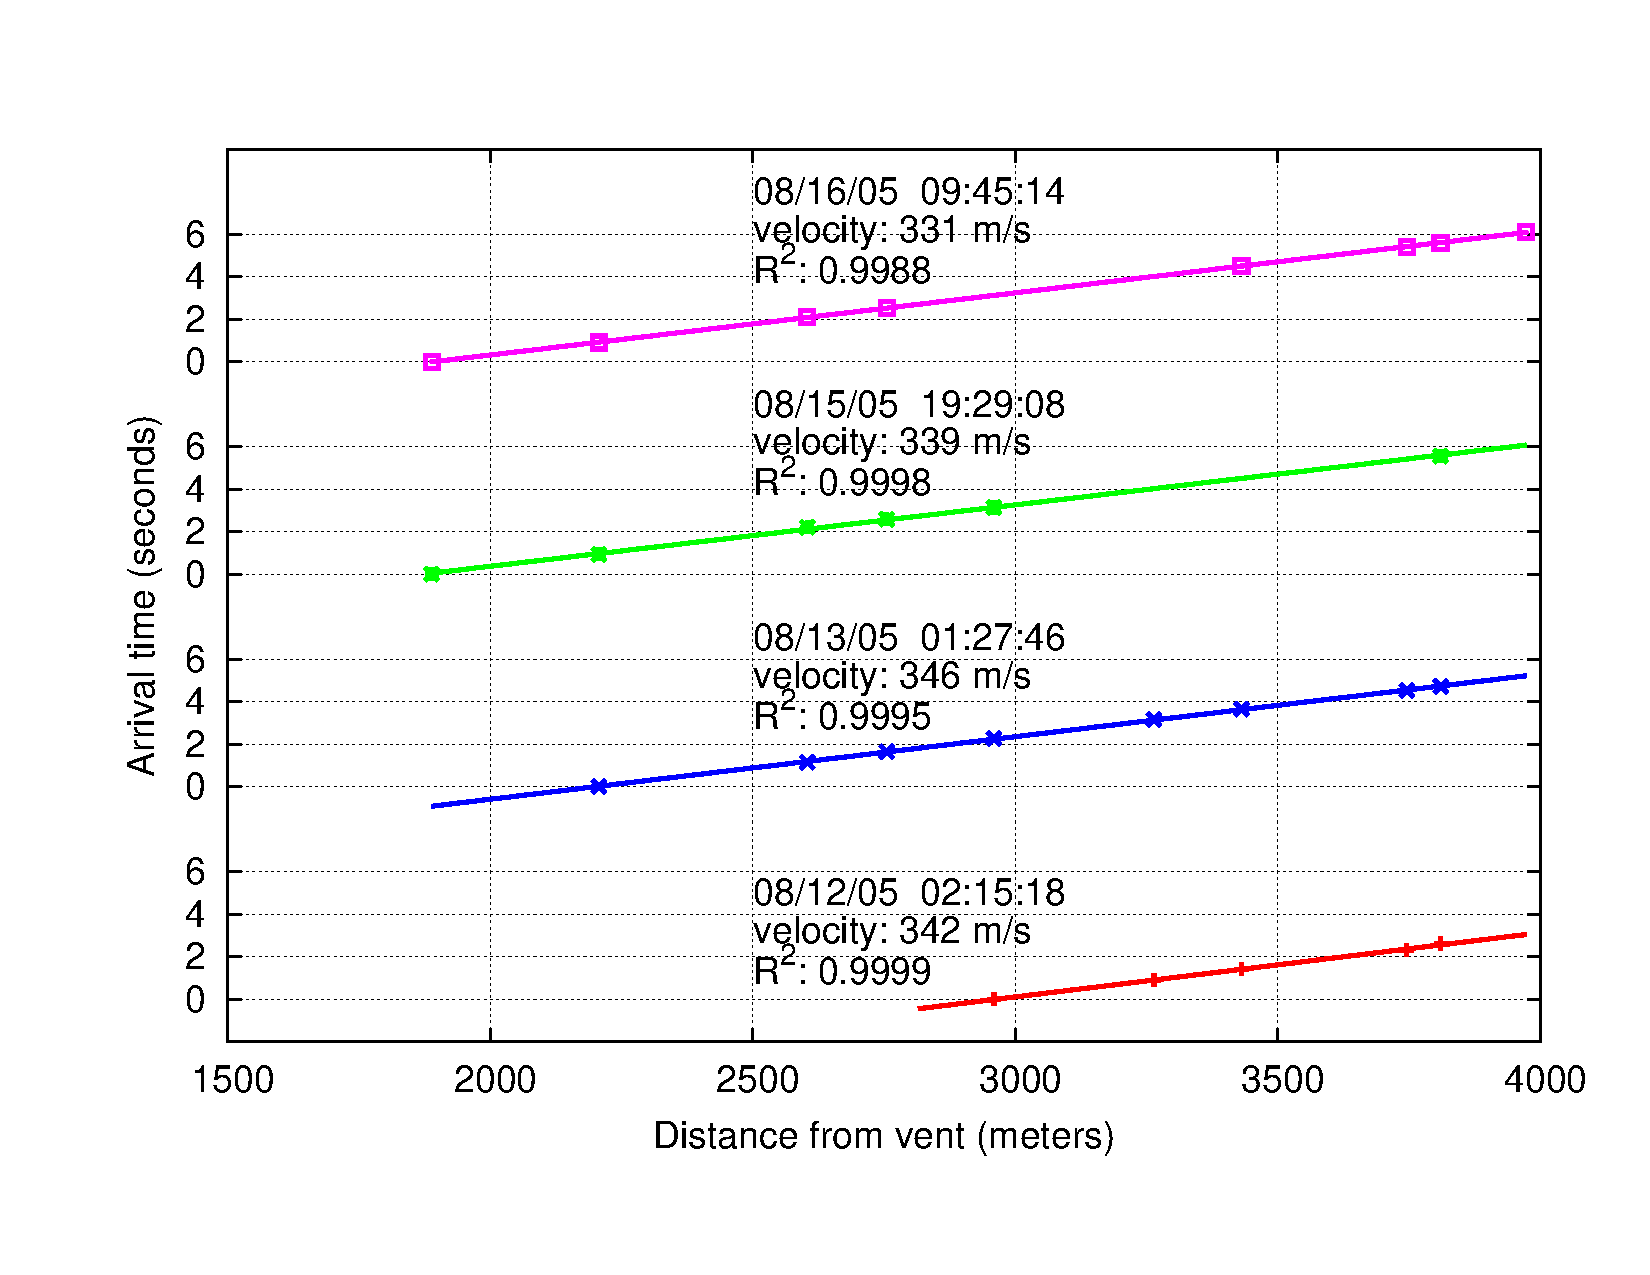
\includegraphics[width=\hsize]{./5-evaluation/figs/fidelity/acousticArrival/acoustic.pdf}
\end{center}
\caption{\textbf{Acoustic wave arrival times and velocity.}
This figure shows the acoustic wave arrival time vs. distance from the vent
for 4~separate events. Also shown is the resulting acoustic wave velocity and
the $R^2$ coefficient of determination.}
\end{figure}

The result of this calculation is also shown in
Figure~\ref{evaluation-fig-acousticArrival}.  The velocity of sound in air is
temperature-dependent; for temperatures between 10--20 $^{\circ}$C the
velocity range is 337--343~m/s.  The calculated wave velocities are mostly in
this range, with a mean of 339.5~m/s. The coefficients of determination $R^2$
are very high, between 0.9988~and~0.9999, showing that the timing and quality
of the acoustic data closely matches our expectation of the infrasonic waves
produced by the volcano.

%\begin{figure}[t]
%  \begin{small}
%    \begin{center}
%      \begin{tabular}{|ccc|} \hline
%               {\bf Event} & {\bf Velocity m/s)} & {\bf $R^2$} \\ \hline
%               08/12/05 02:15:18 & 331 & 0.9988 \\
%               08/13/05 01:27:46 & 339 & 0.9998 \\
%               08/15/05 19:29:08 & 346 & 0.9995 \\
%               08/16/05 09:45:14 & 342 & 0.9999 \\ \hline
%               {\bf Mean} & 339.5 & 0.9995 \\
%               {\bf StdDev} & 6.35 & 0.0005 \\ \hline
%      \end{tabular}
%    \end{center}
%  \end{small}
%  \caption{\small{\bf Acoustic time of arrival summary.}  {\em This
%          table summarizes the acoustic wave velocity and $R^2$ from
%          our linear regression.  The mean velocity for the 4 events
%          is 339.5~$m/s$ which is between the expected velocity of
%          soundm, 337~$m/s$ at 10\textcelsius $ $ and 343~$m/s$ at
%          20\textcelsius. The $R^2$ coefficient is very close to 1.0,
%          indicating a very strong correlation.}}
%  \label{fig-acousticArrivalReg}
%\end{figure}

\subsection{Seismic wave propagation}

Analyzing the seismic waves captured by our network is significantly more
challenging. This is primarily because the source locations of seismic waves
are unknown.  Seismic events may originate at the vent (in the case of an
explosion) or deep within the edifice, producing very different patterns of
P-~and S-wave arrivals at each node. A full seismological analysis of our
data is beyond the scope of this paper. However, we present a high-level
measure of the {\em consistency} of the signals captured by our network: that
is, we evaluate whether the seismic wave arrivals are consistent with
expected volcanic activity.

%% Our sensor array was established in a radial geometry for two primary
%% reasons: (1) to understand the attenuation structure of volcanic
%% explosion earthquakes, and (2) to calculate the seismic wavefield
%% incidence for events occurring near the volcanic conduit. Seismic
%% wavefield incidence is an especially important parameter to recover
%% because it provides us with information about the relative depth of
%% volcanic earthquakes. In addition, knowing the velocity structure of the volcanic edifice 
%% provides important geophysical constraints that are used to assess
%% earthquake source parameters.

%% Our sensor array was established in a radial geometry for two 
%% primary reasons: (1) to understand the attenuation structure of 
%% volcanic explosion earthquakes, and (2) to calculate the seismic 
%% wavefield incidence for events occurring near the volcanic
%% conduit.  
%% %Both seismic attenuation, which is the study of how seismic
%% %ground shaking decreases with propagation distance and frequency
%% %content, and wavefield analyses are the focus of ongoing study with
%% %the collected dataset.
%% Seismic wavefield incidence is an especially important parameter to
%% recover because it provides us with information about the relative
%% depth of volcanic earthquakes.  
%For a simplified 2-D geometry, the apparent velocity $V_a$ of seismic
%wave arrivals across the array is determined by the intrinsic 
%P-wave velocity $V_p$ of the medium and angle of incidence $\theta$ 
%of seismic energy on the array: $V_a = V_p / \cos(\theta)$.  
%Typically depth is hard
%to determine through traditional means because seismic stations at
%volcanoes are most easily deployed around the periphery of the volcano
%(providing good epicentral locations but poor depth constraints).  
%
%Our sensors were deployed along a radial trajectory away
%from the vent in order to calculate the move-out of first arrivals
%(i.e., time distribution of compressional P-Wave first arrivals).
%This allows us to discriminate sources originating in the shallow
%portion of the cone near the vent from events occurring more deeply.
%Furthermore, variations in apparent velocity, calculated from the
%move-out, enable us to estimate origin depth of various events.
%
%For a near-surface source in the vicinity of the
%vent, $\theta$ approaches zero and apparent velocity approaches intrinsic
%compressional velocity of the medium.  Conversely, for a deeper source
%(i.e., volcano-tectonic event), seismic angles can steeply impinge
%upon the free surface of the volcanic edifice leading to infinite
%apparent velocity.  For both types of events presented in Figure 3, the
%lowest apparent velocities (1.5 to 2.0 km/s) is observed towards the
%far end of the array (Figure 3).  This is the value that most closely
%approximates the seismic P-wave velocity of the volcano in this locale.
%% In addition, knowing the velocity structure of the volcanic edifice 
%% provides important geophysical constraints that are used to assess earthquake
%% source parameters.

\begin{figure}[t]
\label{evaluation-fig-seismicArrivalScatteredNode}
\begin{center}
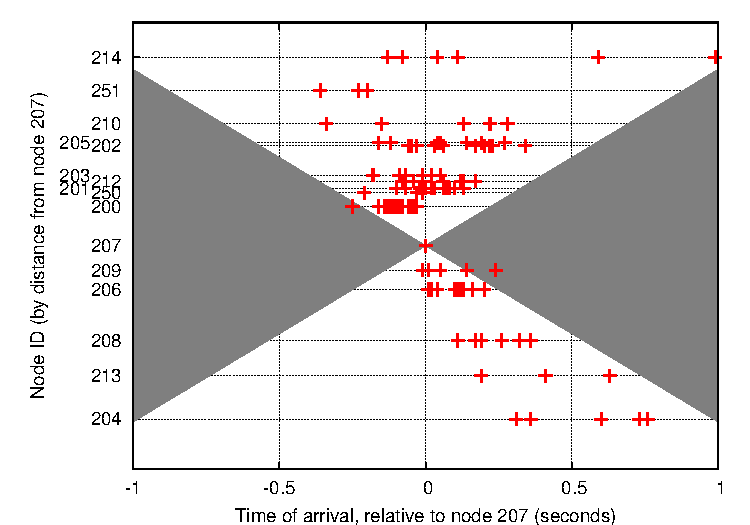
\includegraphics[width=\hsize]{./5-evaluation/figs/fidelity/seismicArrival/arrivalTimesPlotScatteredNode.pdf}
\end{center}
\caption{\textbf{Time of arrival of each node over multiple events.}
This graph shows the spread of arrival times for each node.  The arrival time
and distance is relative to node~207.  The arrival time for each node is
fairly consistent over multiple events, with the exception of node~214.  The
shaded area indicates a move-out velocity of less than 1,500 $m/s$.}
\end{figure}

The most natural measure of data consistency is whether the time of the
seismic P-wave arrival at each sensor falls within an expected {\em envelope}
based on the minimum speed at which seismic waves are believed to propagate
at Reventador, which we estimate as 1500~m/s. We took 15~seismic events with
clear P-wave arrivals and used an automatic algorithm~\cite{pwave-picking} to
determine the wave arrival time.\footnote{Unlike acoustic waves, determining
seismic wave arrival times is notoriously difficult. The seismograms in
Figures~\ref{evaluation-fig-jjExplosion} and
Figure~\ref{evaluation-fig-jjTectonic} should give the reader some
appreciation for this.} 

Figure~\ref{evaluation-fig-seismicArrivalScatteredNode} shows a scatterplot
of the arrival times with respect to node~207, which was chosen as an
arbitrary reference point since data for this node appeared in all 15~events.
The $y$-axis represents the distance of each node from~207. Depending on the
seismic source location, we expect waves to arrive both before and after
node~207.  However, the slowest wave speed (1500~m/s) dictates the maximum
difference in the wave arrival between each station.\footnote{Note that there
is no lower bound on arrival times, since a wave emanating from a deep source
could arrive at all stations nearly simultaneously.} The shaded area in
Figure~\ref{evaluation-fig-seismicArrivalScatteredNode} covers the
``exclusion envelope'' of arrival times at each station.  As the figure
shows, only 2~out of~124 arrivals fall outside of this envelope.

%It is interesting to note that although node~204 is closest
%to the vent, seismic waves do not appear to reach this node first;
%this suggests a deep source under the middle of the sensor array,
%which is by itself an interesting scientific finding.

%The automated picking algorithm uses a tiered approach.  Seismograms
%are initially prepared by extracting the envelope waveform using the
%Hilbert transform.  This is followed by a median smoothing filter to
%remove noise glitches and otherwise undesirable high frequency
%signals.  The smoothed envelopes are then passed through a series of
%gradually refined forward-backward (sometimes called STA/LTA)
%root-mean-square ratio estimate.  Arrival times where significant
%changes in the ratio curves occur are saved.  Several thresholds are
%examined statistically and the initial estimate of the pick is
%determined by robust quantile cut-offs.
%
%This initial arrival time estimate is then used as a first guess
%provided to the so-called ARAIC algorithm (Auto-Regressive Akaiki
%Information Criterion) of Sleeman and van Eck~\cite{pwave-picking}.
%The ARAIC method uses an autoregressive characterization of the noise
%and signal and finds the time along the trace that minimizes the
%maximum likelihood function fit to the AR models.  The algorithms were
%implemented in R~\cite{r-book}, an interactive computation platform.

\begin{figure}[t]
\label{evaluation-fig-jjExplosion}
\begin{center}
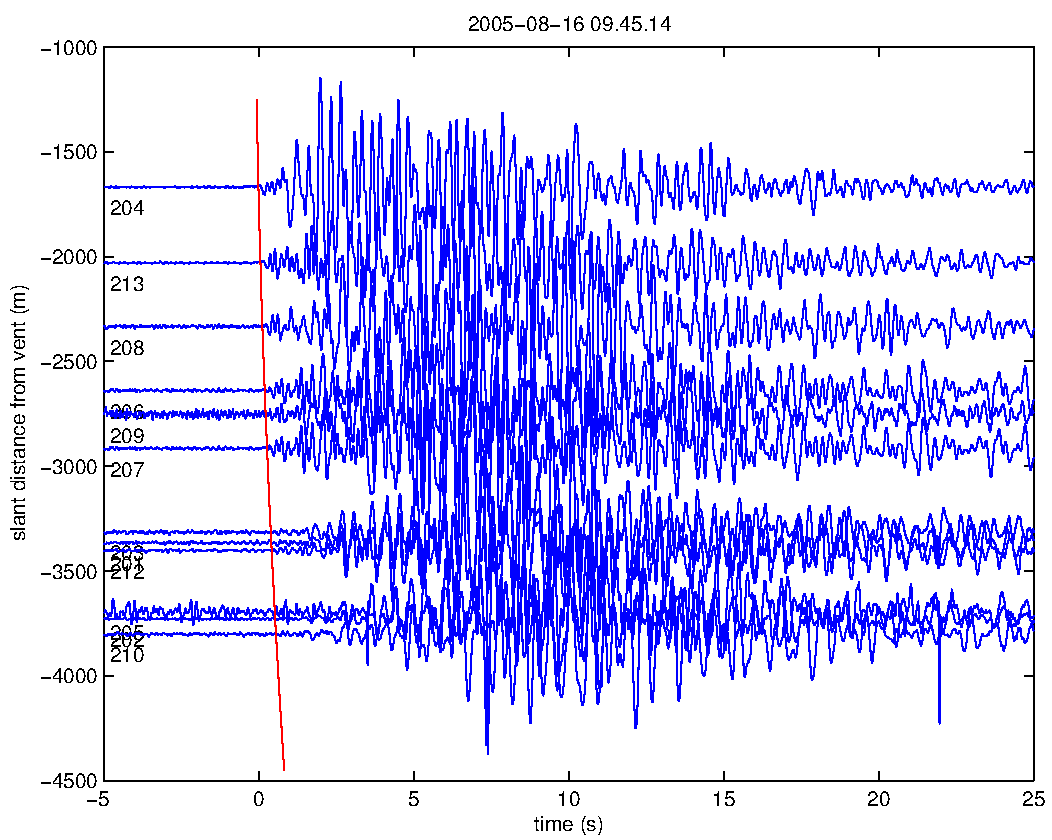
\includegraphics[width=\hsize]{./5-evaluation/figs/fidelity/seismicArrival/johnson/2005-08-16_09-45-14.pdf}
\end{center}
\caption{\textbf{Explosion earthquake event at 08/16/2005 09:45:14 GMT.}
P-wave arrivals have been identified manually and a second-order polynomial
(solid line) is fit to the arrivals. The arrival time move-outs are
consistent with a shallow near-vent source.}
\end{figure}

Finally, we take a closer look at two seismic events recorded by our array.
Figures~\ref{evaluation-fig-jjExplosion}~and~\ref{evaluation-fig-jjTectonic}
show seismograms from each of the sensor nodes after time rectification.  The
$y$-axis corresponds to the distance of each node from the vent.  For each
event, the P-wave arrivals have been determined by hand and a second-order
polynomial has been fit to the arrival times at each node for clarity.

These two events show a very different pattern of wave arrival times.
Figure~\ref{evaluation-fig-jjExplosion} shows the seismic wave arriving first
at stations near the vent (nodes~204 and 213). This is consistent with a
shallow near-vent source corresponding to an explosion. This is confirmed by
the corresponding acoustic data (shown in
Figure~\ref{evaluation-fig-acousticArrival}) attributed to explosive
expansion of gas. 

In contrast, Figure~\ref{evaluation-fig-jjTectonic} shows an event with the
earliest arrivals in the middle of the sensor array and the endpoints
relatively delayed; many such events were recorded by our network.  This
distribution implies a deeper source.  At the same time, seismic velocity in
the uppermost cone, which is comprised of unconsolidated volcanic deposits,
is presumed to be slower.  Such volcano-tectonic events are likely generated
by the fracturing of solid media typically induced by pressurization within
the edifice. This preliminary study demonstrates the value of our wireless
sensor network for collecting accurate signals that can be subjected to
seismological analysis.

\begin{figure}[t]
\label{evaluation-fig-jjTectonic}
\begin{center}
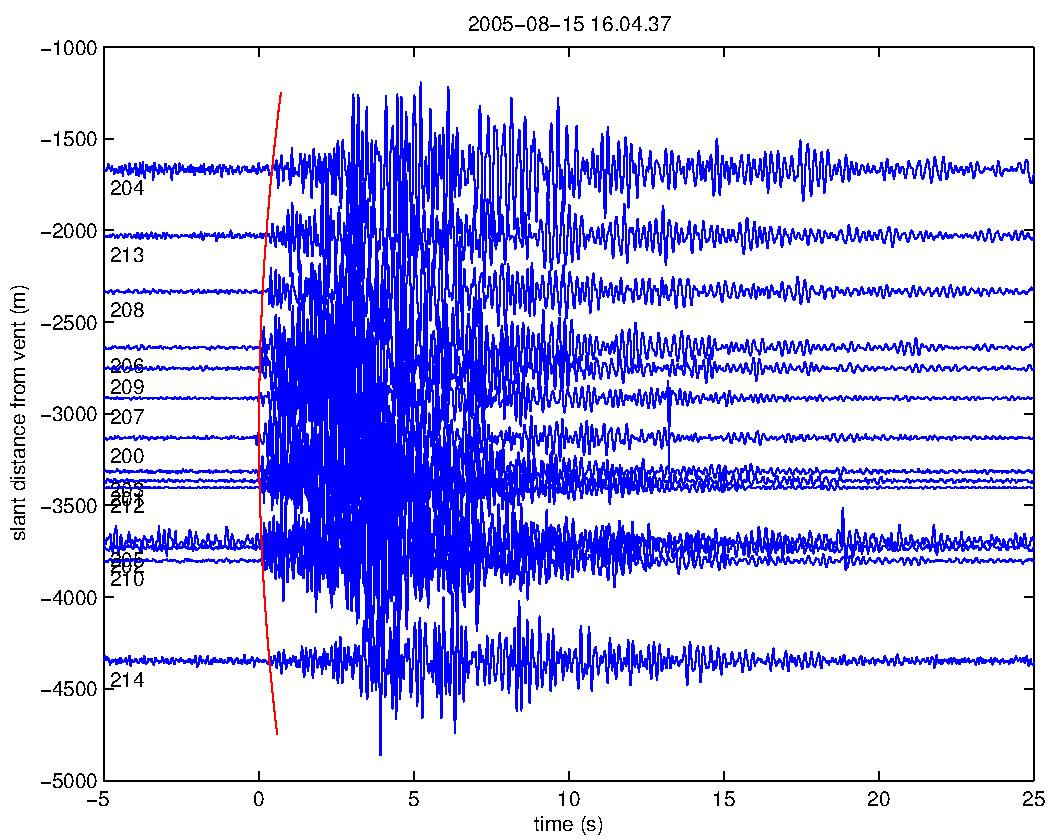
\includegraphics[width=\hsize]{./5-evaluation/figs/fidelity/seismicArrival/johnson/2005-08-15_16-04-37.pdf}
\end{center}
\caption{\textbf{Tectonic earthquake event at 08/15/2005 16:04:37 GMT.}
In this event, seismic waves are first recorded near the middle of the sensor
array. This is due either to a source closer to the center of the array,
variations in velocity structure, or most likely both.}
\end{figure}


%%%%%%%%%%%%% OLD text %%%%%%%%%%%%%%%%%%%%%%%%
% - How different from acoustic
% - Subset of events that we analyzed
% - How we did linear fit and table fo results

%% \begin{figure}[t]
%% \begin{center}
%% 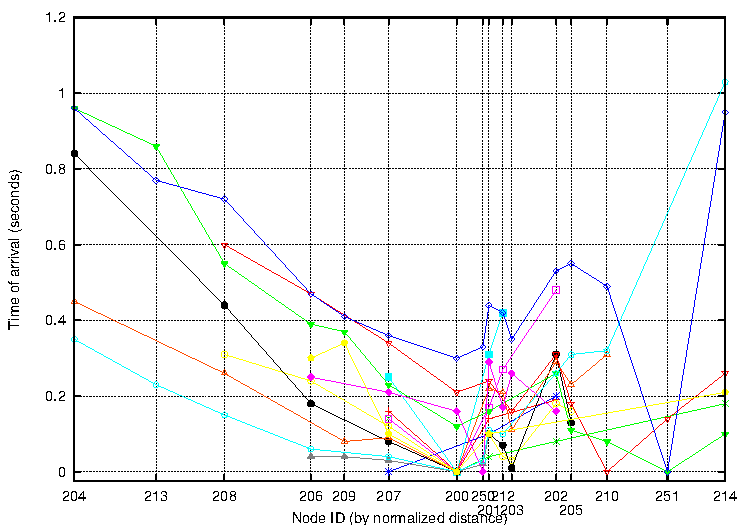
\includegraphics[width=\hsize]{./5-evaluation/figs/fidelity/seismicArrival/arrivalTimesPlot.pdf}
%% \end{center}
%% \caption{\small{\bf Time of arrival for the seismic data.}
%% {\em This figure shows the seismic wave arrival time offset by the
%% first arrival vs. normalized distance between nodes.  The graph indicates that
%% most events originate closer to the center of the array.}}
%% \label{fig-seismicArrival}
%% \end{figure}

%% \begin{figure}[t]
%% \begin{center}
%% 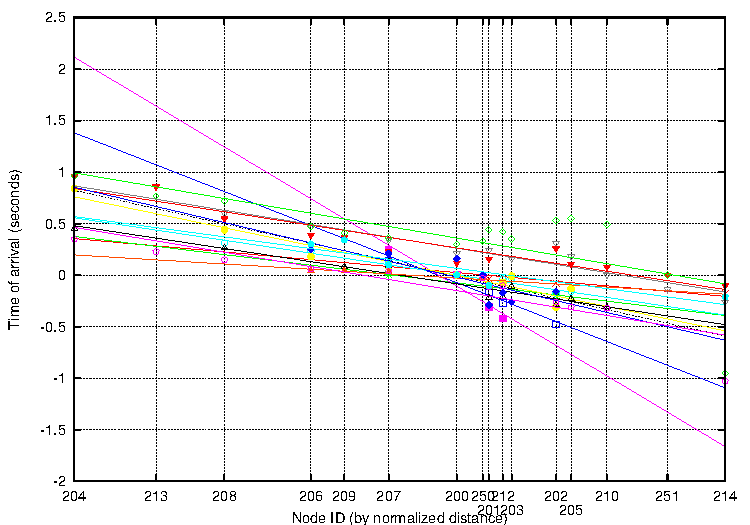
\includegraphics[width=\hsize]{./5-evaluation/figs/fidelity/seismicArrival/arrivalTimesPlotFit.pdf}
%% \end{center}
%% \caption{\small{\bf Liner regression for the time of arrival for the seismic data.}
%% {\em This arrival times of nodes to the right of the node with
%% the first arrival are mirrored about the x-axis.  This allows us to
%% draw a linear fit through the data points.  As we can see, most events
%% have a similar slope which indicates consistent wave velocities.}}
%% \label{fig-seismicArrivalFit}
%% \end{figure}

%% \begin{figure}[t]
%% \begin{center}
%% 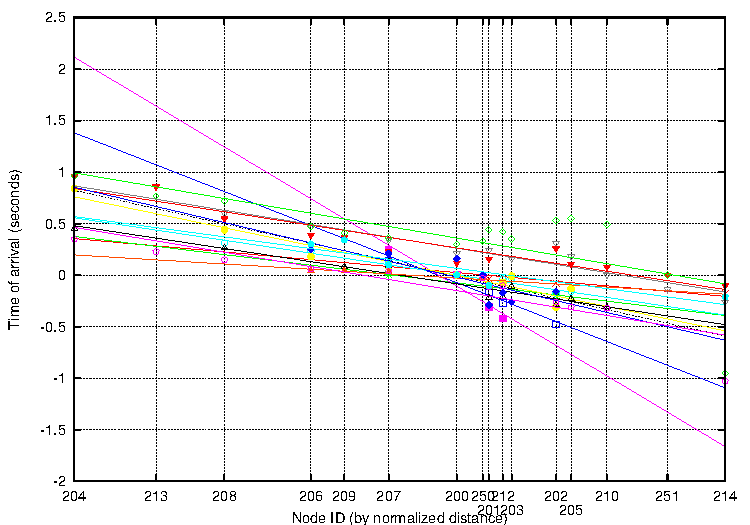
\includegraphics[width=\hsize]{./5-evaluation/figs/fidelity/seismicArrival/arrivalTimesPlotFit.pdf}
%% \end{center}
%% \caption{\small{\bf Liner regression for the time of arrival for the seismic data.}
%% {\em This arrival times of nodes to the right of the node with
%% the first arrival are mirrored about the x-axis.  This allows us to
%% draw a linear fit through the data points.  As we can see, most events
%% have a similar slope which indicates consistent wave velocities.}}
%% \label{fig-seismicArrivalFit}
%% \end{figure}

%% \begin{figure}[t]
%% %  \begin{minipage}[t]{.45\textwidth}
%%   \begin{small}
%%     \begin{center}
%%       \begin{tabular}{|ccc|} \hline
%%                {\bf Event} & {\bf Velocity (m/s)} & {\bf $R^2$} \\ \hline
%%                2005-08-11\_08.33.49 & 2356.97 & 0.91 \\
%%                2005-08-11\_09.12.38 & 5519.13 & 0.89 \\
%%                2005-08-11\_15.04.27 & 4287.73 & 0.99 \\
%%                2005-08-12\_00.30.40 & 1324.12 & 0.96 \\
%%                2005-08-12\_02.15.18 &  832.95 & 0.93 \\
%%                2005-08-13\_02.17.32 & 3376.40 & 0.96 \\
%%                2005-08-13\_04.24.42 & 2406.30 & 0.94 \\
%%                2005-08-13\_07.08.05 & 3241.98 & 0.95 \\
%%                2005-08-14\_04.32.29 & 8204.96 & 0.67 \\
%%                2005-08-14\_20.17.02 & 3061.23 & 0.87 \\
%%                2005-08-15\_09.11.28 & 3175.71 & 0.89 \\
%%                2005-08-15\_16.04.37 & 2903.11 & 0.51 \\
%%                2005-08-16\_01.32.19 & 2173.40 & 0.65 \\
%%                2005-08-16\_18.30.04 & 2981.71 & 0.77 \\
%%                2005-08-18\_02.45.51 & 3621.04 & 0.81 \\ \hline
%%       \end{tabular}
%%     \end{center}
%%   \end{small}
%%   \caption{\small{\bf Coefficient of determination ($R^{2}$) for events.}
%%           {\em The coefficien of determination is a measure of how well the
%%           regression line represents the data.  A coefficient value greater than
%%           0.65 is generally described as a strong correlation.  As we can see,
%%           most of our events have a coorelation higher than 0.65 indicating a good fit.}}
%%   \label{fig-seismicArrivalReg}
%% %  \end{minipage}
%% \end{figure}


%% \begin{figure}[t]
%% \begin{center}
%% 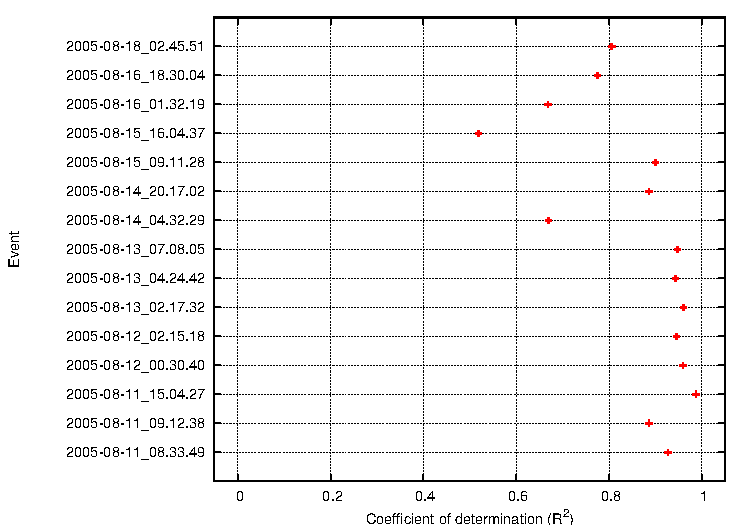
\includegraphics[width=\hsize]{./5-evaluation/figs/fidelity/seismicArrival/arrivalTimesPlotReg.pdf}
%% \end{center}
%% \caption{\small{\bf Coefficient of determination ($R^{2}$) for events.}
%% {\em The coefficien of determination is a measure of how well the
%% regression line represents the data.  A coefficient value greater than
%% 0.65 is generally described as a strong correlation.  As we can see,
%% most of our events have a coorelation higher than 0.65 indicating a good fit.}}
%% \label{fig-seismicArrivalReg}
%% \end{figure}


%% \begin{figure}[t]
%% \begin{center}
%% 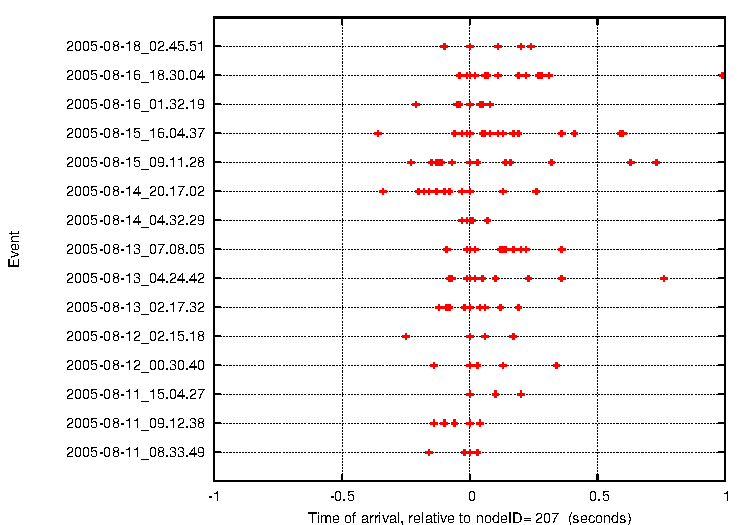
\includegraphics[width=\hsize]{./5-evaluation/figs/fidelity/seismicArrival/arrivalTimesPlotScatteredEvent.pdf}
%% \end{center}
%% \caption{\small{\bf Time of arrival of nodes for each event.}
%% {\em This graph shows the spread of arrival times.  The arrival times
%% are relative to node 207.  As we can see, most arrival times are
%% within a 1 second window of each other with a few outliers.}}
%% \label{fig-seismicArrivalScatteredEvents}
%% \end{figure}

%\begin{figure}[t]
%\begin{center}
%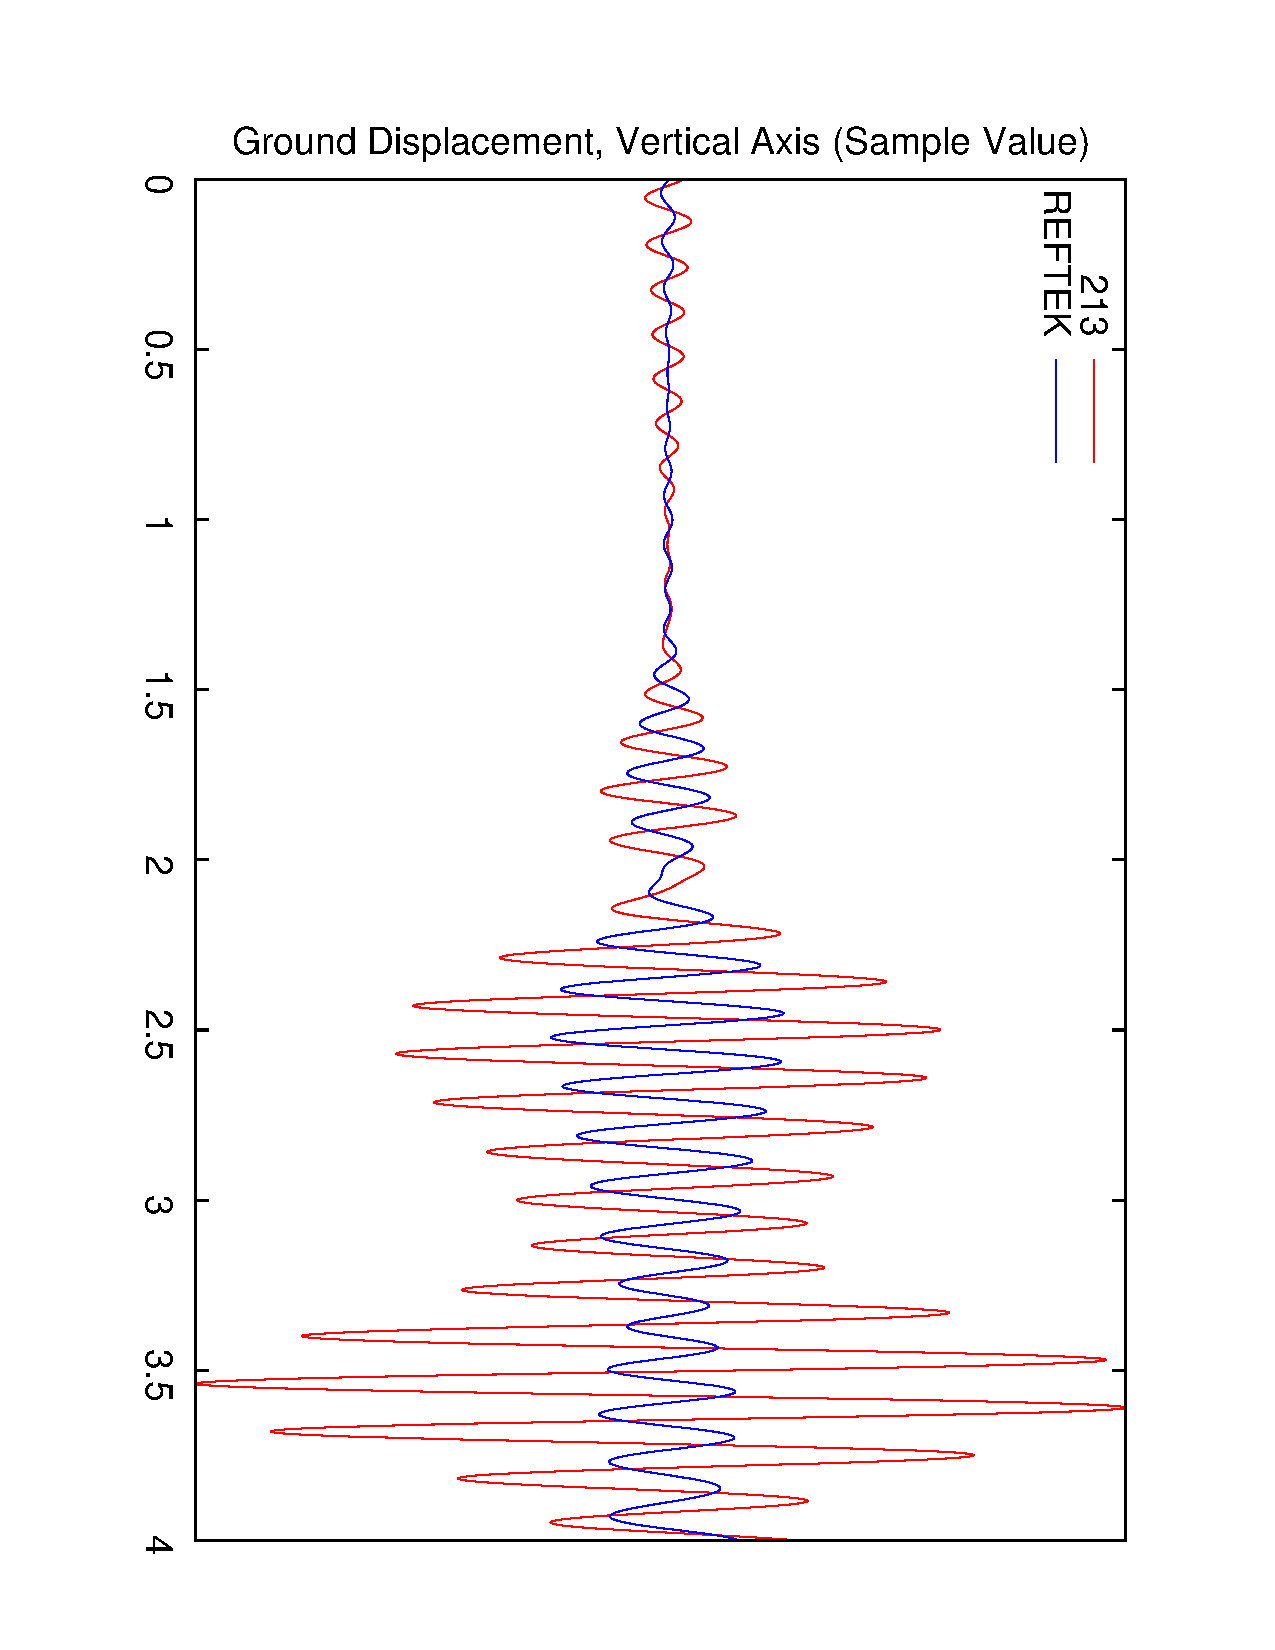
\includegraphics[width=0.8\hsize,angle=90]{./5-evaluation/figs/timing/RV213/2005-08-15_16.04.37/213VREFTEK-NO-OFFSET.pdf}
%(a)
%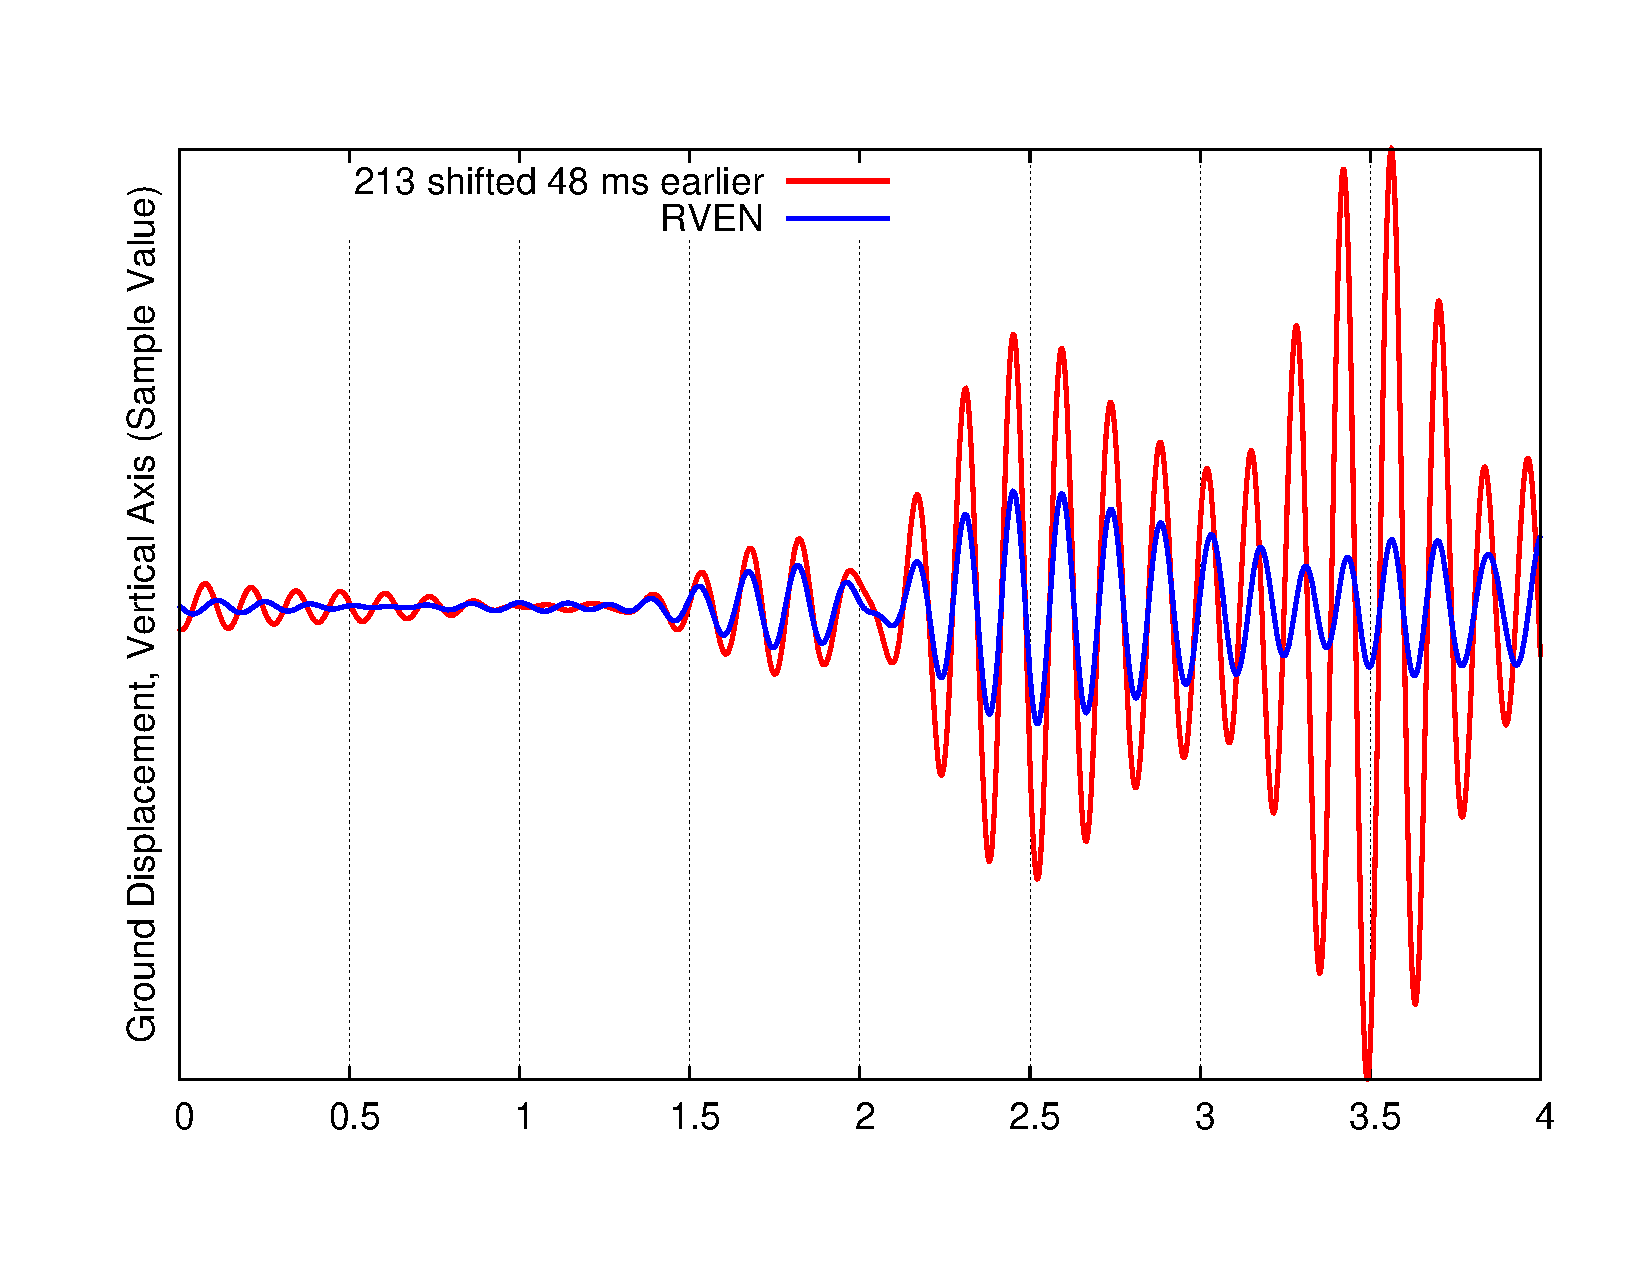
\includegraphics[width=0.8\hsize,angle=90]{./5-evaluation/figs/timing/RV213/2005-08-15_16.04.37/213VREFTEK-POSITIVE48MS-OFFSET.pdf}
%(b)
%\end{center}
%\caption{\small{\bf Comparison of Node 213 and Reftek Signals}
%{\em The figures above show two signals, one collected by a sensor
%network station, Node 213, the other collected by a Reftek data logger
%attached to a broadband seismometer. Figure (a) shows the signals before a
%shift is applied, and Figure (b) shows the signals with a 48 ms shift
%applied. Both signals have been bandpass filtered between 6 and 8 Hz to
%reduce the differences in instrument response.  As these figures show a 48 ms
%shift produces a good match at the arrival time of the energy.  The
%signals are expected to differ throughout the coda showing the arrival of
%S-waves. \GWAnote{Need a better way to describe this...}}}
%\label{fig-rvenv213}
%\end{figure}


\section{Related Work}
\label{sec-relatedwork}

This section discusses four kinds of related systems, those designed to cope
with high data rates, designed to operate in scientific contexts, and related
to Lance or IDEA.

\subsection{High Data Rate Sensing}

Many sensor network applications require collecting high-resolution signals
using low-power nodes. Examples include monitoring acoustic, seismic, and
vibration waveforms in bridges, industrial equipment, and animal habitats.
These systems all attempt to acquire high data rate (100~Hz or higher),
high-fidelity data across the network subject to severe constraints on radio
bandwidth and energy usage.

A group from UC Berkeley performed the largest deployment to date of sensor
network nodes for structural health monitoring: 46 nodes placed on the Golden
Gate Bridge~\cite{ggb-ipsn07}. Nodes collect vibration data at 1~kHz, and the
network uses many of the same routing and time synchronization protocols used
by our volcano monitoring system. A special bulk data collection protocol,
called Straw, was developed for the deployment. The highly linear topology of
the deployed network was later used to test the Flush data collection
protocol~\cite{flush-sensys07}. The deployment at the Golden Gate Bridge also
gave rise to a system called the Structural Health Monitoring Toolkit
(Sentri) that interfaces between the outside world and the sensor network by
transmitting commands to nodes as necessary.

NetSHMis a wireless sensor network for structural health monitoring, which
involves studying the response of buildings, bridges, and other structures to
localize structural damage, e.g., following an
earthquake~\cite{netshm-ewsnsubmission,netshm-emnets05,wisan}. This system
shares many of the challenges of geophysical monitoring. Indeed, the data
rates involved (500~Hz per channel) are higher than are typically used in
volcano studies. The Wireless Modular Monitoring System (WiMMS) is another
structural monitoring network with similar goals that has been validated both
in field deployments at the Geumdang Bridge in Icheon, South Korea, and in
laboratory tests~\cite{wimms-lynch06}. This system is designed to supporting
decentralize control algorithm that respond to structural changes using
actuators. In this context decentralization reduces the amount of data that
must be transmitted to a central location while eliminating the base station
as a single point of failure.

NetSHM implements reliable data collection using both hop-by-hop caching and
end-to-end retransmissions. The work explores the use of local computations
on sensors to reduce bandwidth requirements. Rather than a global
time synchronization protocol, the base station timestamps each sample upon
reception. The \textit{residence time} of each sample as it flows from sensor
to base is calculated based on measurements at each transmission hop and used
to deduce the original sample time.

Several factors distinguish our work on volcano science from structural
monitoring applications. First, structural monitoring networks typically
either collect data following controlled excitations of a structure or at
periodic intervals, which simplifies transmission scheduling. In our case,
volcanic activity is bursty and highly variable, requiring more sophisticated
approaches to event detection and data transfer. While the Golden Gate Bridge
system is sparsely deployed like our volcano sensor networks, many structural
monitoring applications are deployed in relatively dense networks, making
data collection and time synchronization more robust. 

Condition-based maintenance is another emerging area for wireless sensor
networks. The typical approach is to collect vibration waveforms from
equipment (e.g., chillers, pumps, etc.) and perform time- and
frequency-domain analysis to determine when the equipment requires servicing.
Intel Research has explored this area through deployments at a fabrication
plant and an oil tanker in the North Sea~\cite{intel-northseasensys}.
Although this application involves high sampling rates, it does not
necessarily require time synchronization as signals from multiple sensors
need not be correlated. The initial evaluation of these deployments only
considers the network performance and does not address data fidelity issues.

While many early environmental monitoring applications are characterized by
low data rates, some have focused on applications requiring high-speed data
acquisition. An example application is monitoring colonies of marmots. A
group at MIT led by Lew Girod has explored several generations of hardware
and software solutions for distributed acoustic monitoring driven by this
application~\cite{girod-marmots}. This work produced the Acoustic
ENSBox~\cite{girod-ensbox}, a self-calibrating hardware solution designed to
be easy to deploy in support of acoustic sensing applications. The ENSBox
features an ARM processor, which puts it at a different point on the
power-performance curve from typical sensor network nodes and makes it more
suitable for the high-speed processing necessary to capture acoustic signals.

The software environment for the ENSBox was originally provided by
EmStar~\cite{emstar}, which targets Linux-based platforms. More recently, the
ENSBox has been used as the basis of the VoxNet platform, an environment
designed for acoustic signal collection and processing.
VoxNet~\cite{voxnet-ipsn08} is comprised of three pieces:
Wavescope~\cite{wavescope}, a programming environment targeting
heterogeneous sensor networks. Wavescope programs are written in
WaveScript~\cite{wavescript-techreport08}, a stream-processing language.
Users compose a set of filters and other stream operators into a ``script''
similar to a data-flow graph.

The VoxNet platform includes a variety of network services, such as
time synchronization, routing, and node localization that applications
running in this environment can make use of. Once the program is written and
installed on nodes, VoxNet includes a set of control and visualization tools
intended to allow users to interact with the running system and view the data
as it is collected. A system using VoxNet was deployed in 2008 at the Rocky
Mountain Biological Laboratory and used to study the alarm calls of marmots.
Acoustic monitoring has scientific applications to other species as well, as
a variety of animals and birds produce scientifically-interesting
vocalizations.

Another application of high data rate sensing to habitat monitoring is the
cane toad monitoring project run by a team at Portland State University,
CSIRO, and the University of New South Wales. The cane toad is an invasive
species in Australia, and their spread is being monitored due to concerns
about their impact on the country's native fauna. The goals of the project
are to design a system permitting \textit{in situ} classification of various
frog species based on their vocalizations.

After completing a pilot study, two additional iterations advanced the design
of the system. In the first, a hybrid network was developed, mating low-power
sensor nodes and middle-tier devices with more advanced processing and
storage capabilities. Data reduction is performed on the sensor nodes in
order to limit the amount of information that must be sent to the high-power
devices, thus prolonging the lifetime of the embedded
nodes~\cite{canetoad-tosn}. The second iteration explores compressive
sampling techniques and also deploys a classification algorithm that can be
run directly on the resource-constrained sensor nodes.

Camera-based sensor networks also produce high data rates and have been the
subject of considerable study. A group at UCLA built a system called
Cyclops~\cite{cyclops-sensys05} which brings vision technology to sensor
network devices by offering a low-power imaging devices better suited to mating
with resource-constrained sensor nodes. They show that Cyclops nodes can
successfully perform fundamental vision-recognition tasks such as object
detection and hand posture recognition. Another team at UMass Amherst sees
motes fitted with imagers as forming one tier of a multi-tier multi-modal
($M^2$) sensor network~\cite{m2-nossdav05}. Such $M^2$ networks consist of
several tiers operating at different power levels while attempting to combine
the capabilities of multiple types of devices. The lowest tier might consist of
low-power sensor nodes equipped with vibration sensors and be used to trigger
the operation of more power-hungry devices --- such as
Stargates~\cite{stargate} fitted with webcams --- in the upper tiers.

\subsection{Scientific Sensing}

The first generation of sensor network deployments focused on distributed
monitoring of environmental conditions. Representative projects include the
Great Duck Island~\cite{spm:04habitat,polastre-masters,mainwaring-habitat},
Berkeley Redwood Forest~\cite{berkeley-redwoods}, and James
Reserve~\cite{cerpa-habitat} deployments. These systems are characterized by
low data rates (sampling intervals on the order of minutes) and very
low-duty-cycle operation to conserve power. Research in this area has made
valuable contributions in establishing sensor networks as a viable platform
for scientific monitoring and developing essential components used in our
work. 

This previous work has not yet focused on the efficacy of a sensor network as
a scientific instrument. The best example is the Berkeley Redwood Forest
deployment~\cite{berkeley-redwoods}, which involved 33~nodes monitoring the
microclimate of a redwood tree for 44~days. Their study focuses on novel ways
of visualizing and presenting the data captured by the sensor network, as
well as on the data yield of the system. The authors show that the
microclimactic measurements are consistent with existing models, but ground
truth of the data is not established. This paper does highlight many of the
challenges involved in using wireless sensors to augment or replace existing
scientific instrumentation.

A group at UCLA has built a system for soil monitoring and deployed it in the
AMARSS transect in the James Reserve, a biological field station operated by
the University of California. The goal was to augment a set of wired data
loggers with wireless sensor technology, similar in spirit to what we have
attempted with our volcano monitoring system. Since 2005 the deployed system
has collected over 26~million measurements, which are retrieved periodically
by a technician visiting the deployment site. The goal is to study the carbon
cycle and estimate the flux of carbon dioxide from the soil.

The largest challenge facing these researchers was coping with missing data.
To address it, they built a system called Suelo~\cite{suelo-sensys09}.  Suelo
is intended to aid human researchers in monitoring and assisting the health
of the deployment, sense the soil-monitoring sensors used are quite fragile.
Suelo monitors the readings capture by the network and tries to distinguish
between ``interesting'' and ``faulty'' data, and initiating human
intervention when sensors require replacement or recalibration.

Computer scientists at UMass Amherst have been deploying GPS-enabled sensors
to study the movement of a threatened species of turtle. This work led to
Eon, a language and runtime system designed to enable energy-aware
programming. Eon claims to be the first energy-aware programming language and
tries to make resource usage explicit to programmers by allowing them to
annotate their code with energy states. At runtime, Eon will adapt the
behavior of the node based on resource availability.

Similar to our work in its application to environmental hazard mitigation,
previous projects have explored sensor networks for flood and landslide
detection, at MIT and John Hopkins University, respectively. The MIT system
feeds data from a network of sensors into a model designed to predict
rainfall-triggered flooding~\cite{basha-sensys08}. They were able to show the
demonstrate the accuracy of their approach using data collected over multiple
field deployments on Honduras between 2004 and 2007. JHU's approach to
landslide detection employs sensor columns, vertical underground
installations of several different sensors~\cite{landslide-sensys05}. When a
portion of the deployed network detects that a slip surface is forming, nodes
cooperate to estimate the position of the slip surface which is fed into a
model that predicts whether and when a landslide will occur. Both of these
projects differ from our work by involving significant modeling and
prediction components, whereas we have focused primarily on raw data
collection.

Of particular interest is ongoing work at Washington State University using
camera-dropped sensor networks to monitor the activity of Mt. St.
Helens~\cite{wsuvolcano-mobisys09}. This project shares many of our goals,
including ease of deployment and data fidelity, but differs in its focus on
system lifetimes of up to 1~year, and in its aim to replace, rather than
augment, existing volcano monitoring stations. The reliance on helicopter
support while deploying nodes also leads to a different set of design
decisions, including much larger batteries and more capable nodes.

The WSU group uses an iMote2~\cite{imote2} sensor node, which shares the
CC2420 802.15.4 radio with our TMote but features the PXA271 XScale processor
with significantly more computational horsepower than the MSP430. The
expanded form factor and power budget permits the use of GPS at each node,
simplifying time sychronization (although FTSP is available as a backup if
the GPS signal is lost).

While the system aims to provide continuous data collection, the limited
bandwidth of the 802.15.4 radios on each sensor node and the 900~MHz
Freewave~\cite{freewave} modem used to maintain a connection with the
observatory limit the data that can be collected. Similar to our
volcano-monitoring system, an impulse detector implemented as a short-term
average over long-term average (STA/LTA) is used to assign a priority to the
data as it is collected. Data prioritization is used during data collection
and routing to ensure that data from detected events reaches the observatory
first. Currently the system works around energy limitations by using heavy
AIR-ALKALINE batteries, which are feasible because the nodes are being
deployed by helicopter.

\subsection{Data Quality Optimization Frameworks}
\label{lance-sec-related}

Several systems are related to Lance but differ substantially in their goals
and assumptions.

EnviroMic~\cite{enviromic} is a system designed to support distributed
acoustic recording by leveraging the collective storage resources of multiple
sensor nodes. It performs cooperative recording by organizing nodes into
groups when multiple nodes detect the same acoustic event, and using these
groups to ensure that only one node is recording acoustic data for as long as
the event of interest continues. This is intended to reduce the amount of
data that must be stored by eliminating redundant signal collection.

EnviroMic also focuses on distributing the storage load within the network to
ensure that the distributed storage can be utilized and signals of interest
not lost due to full Flash drives. While nodes may exchange data to rebalance
storage during the experiment, the fundamental assumption of the architecture
is that data will be manually retrieved from sensor nodes following the
deployment. Unlike Lance, EnviroMic is not intended for applications with
real-time data needs.

ICEDB~\cite{zhang2007icedb} supplies a delay-tolerant and priority-driven
query processor for the CarTel~\cite{cartel} system. ICEDB provides SQL
extensions allowing queries to assign both inter- and intra-stream
priorities, which are used by the query processor to manage bandwidth and
storage resources. ICEDB also uses a similar node-level summarization
technique to that used by Lance.

While ICEDB considers bandwidth limitations, it does not consider energy as a
constraint. The fundamental goal of ICEDB --- to provide database-like access
to mobile nodes that may experience periods of disconnection or poor
connectivity --- differs from that of Lance, which explains the architectural
differences. CarTel nodes are much higher-power and assumed to be attached to
power sources in the vehicles that they are deployed in.

VanGo~\cite{vango} provides an architecture for collecting and processing
high-resolution sensor data on resource-constrained nodes. VanGo focuses on a
programming model based on a linear filter chain and implementing efficient
signal-processing operations with limited computational power.
WaveScope~\cite{wavescope} and Flask~\cite{flask-tr} are languages for stream
processing applications. These systems are largely complementary to Lance,
and could be used to process signal data prior to collection, although our
focus is on collecting \textit{raw} sensor data from large networks. These
systems do not attempt to optimize data collection under varying energy and
bandwidth constraints. 

\subsection{Energy Load-Balancing Services}
\label{idea-sec-related}

Previous work has addressed the problem of energy load balancing in contexts
such as sensor coverage, role assignment, and energy-aware routing. Other
efforts in sensor networks have focused on reducing the power consumption at
individual nodes without considering energy distribution. Many of these
efforts are specific to a particular application or component and do not
provide a service like IDEA that can be used by a variety of applications. 

A number of existing systems such as Odyssey~\cite{odyssey-osr99},
PowerScope~\cite{powerscope-wmcsa99} and more recently
Cinder~\cite{cinder-mobiheld09}, have addressed measuring or adapting to
energy variations on battery-powered devices, primarily to support mobile
applications. This naturally produces a difference in approach from IDEA,
since IDEA targets networks consisting of multiple nodes but treated as a
single entity. Since nodes are collaborating we can enable more sharing and
ask nodes to sacrifice for each other, whereas mobile device users would
likely be upset if they discovered that their phone was running low on power
because it was trying to improve the lifetime of a stranger's phone located
nearby.

Quanto~\cite{quanto-osdi08} provides a framework for tracking and
understanding energy consumption in embedded sensor systems. The existence of
systems such as Quanto was a primary motivation for IDEA, since the
visibility distributed resource tracking provides creates an opportunity to
adapt to changes in availability across the network. Currently IDEA requires
that components model their own energy consumption, which may be difficult
for components with complex behavior. We are exploring integrating Quanto
into IDEA to provide more precise tracking of energy at runtime, which could
eliminate the need for component-specific modeling and ease the process of
integrating applications with IDEA.

Eon~\cite{eon-sensys07} performs similar energy tracking and forward
projection but focuses on single-node, not network-wide adaptations.
SORA~\cite{sora-nsdi05} focuses on decentralized resource allocation based on
an economic model in which nodes respond to incentives to produce data or
perform specific tasks, with each node trying to maximize its profit for
taking a series of actions. While SORA, using correctly set prices, could
produce similar network-wide behavior to that enabled by IDEA, the connection
between prices and the behavior of the network is not completely clear. IDEA
simplifies the problem of global network control through the energy objective
function which encapsulates the application's goal.

Some work on energy-aware routing~\cite{ShahRabaey2002,381685} has addressed
equitable energy distribution within the network by probabilistically
choosing between multiple good paths between each source and sink pair.
LEACH~\cite{leach} and other similar approaches attempt to distributed energy
in an entirely decentralized way, using local heuristics to do so.
Lexicographically maximum rate allocation~\cite{fairrate-sensys08} uses a
decentralized algorithm to tune optimum data collection rates in perpetual
networks when static routes are used, all nodes route to a single sink, and
the recharging profiles of the nodes are known ahead of time. Rate allocation
could be implemented in IDEA and comparing the two is planned future work.

VigilNet~\cite{vigilnet} is a target-tracking system that attempts to save
energy by rotating ``sentry'' duties between a group of nearby nodes. Nodes
that are not assigned as sentries can sleep and conserve energy while the
sentry monitors the area. When an event occurs, the sentry awakes nearby
nodes and initiates the tracking process. VigilNet assigns sentry duties
based on each node's energy availability while trying to ensure that the
entire area being monitoring is covered. Given the desire both to extend
system lifetime and maintain a desired application fidelity, VigilNet could
be implemented using IDEA, allowing both energy availability and harvesting
to be considered when assigning setries.

EnviroMic~\cite{enviromic} is a distributed acoustic storage system for
sensor networks. When EnviroMic nodes hear an acoustic event, a leader is
elected to assign recording tasks to nodes in the group. As storage space is
limited, EnviroMic attempts to push data to quiet sections of the network
with unused storage, balancing storage consumption across the network. Both
of these tasks involve choosing from a set of nodes that can perform the same
storage task, and so EnviroMic could be integrated with IDEA allowing the
energy overheads of data transfers to be considered.

The IDEA architecture emerged from our own prior work on energy management
for wireless sensor networks, including Lance (Chapter~\ref{chapter-lance})
Pixie~\cite{pixie-sensys08}, and Peloton~\cite{peloton-hotos09}. Pixie
proposed an operating system and programming framework for sensor network
nodes that promotes resources to a first-class primitive, using tickets to
manage resource consumption and brokers to enable specialized management
policies. Pixie does not consider the energy impact of a node on other nodes.

Peloton proposed an architecture for distributed resource management in
sensor networks combining state sharing, vector tickets to represent
distributed resource consumption and a decentralized architecture in which
nodes serve as ticket agents managing the resource consumption of themselves
and on behalf of nearby nodes. IDEA shares many features with Peloton and can
be viewed as the beginnings of an implementation of the Peloton design, with
state sharing to enable energy decision making and every node serving as a
ticket agent for itself but considering the distributed impact of its own
local state.

%\section{Conclusions}
\label{sec-conclusions}

\section{Lessons Learned}
\label{sec-lessons}

% MDW: I wanted to reword this since the tone was a bit lofty ("we
% spent all this time/money so you can save some of yours...") 
Sensor network deployments, particularly in remote areas, involve 
significant cost in terms of time and equipment. Failures of hardware
and software can have a negative impact on the uptake of this technology 
by domain science experts. Our experiences at Reventador have yielded 
a number of valuable lessons for future sensor network deployments. 

%\begin{itemize}

%\item 
{\bf 1. Ground truth and self-validation mechanisms are critical:}
We did not initially consider colocating several of our wireless
sensors with existing data loggers in order to establish ground
truth. This would have clearly aided our analysis, though we 
were fortunate to locate one of
our sensors near (but not immediately adjacent to) the RVEN station.
%validate the system output we should have planned to colocate trusted, wired
%data loggers alongside several of our stations. This would have made the time
%synchronization and data validity analyses much easier.  
In addition, self-validation mechanisms are needed to provide detailed
information on the health and accuracy of the data recorded by the
network. The periodic ``heartbeat'' messages that we built into our 
system proved essential to remotely tracking system operation.

%\item 
{\bf 2. Coping with infrastructure and protocol failures:} As discussed
previously, the sensor nodes themselves were the most reliable 
components of the system. Even without classifying the 3-day network outage 
as an infrastructure failure, this downtime was far exceeded by outages 
caused by power failures at the base station. 
% MDW: Gotta keep in mind that many folks reading this paper are quite
% senior and will have "seen it all" - let's not be preachy.
We did not devote enough attention to assuring the reliability of the
base station and radio modem infrastructure, assuming it would be a
trivial matter of plugging into wall power. This single point
of failure was more fragile than expected.

Additionally, several pieces deployed software, including Deluge and FTSP,
exhibited failures in the field than we not had expected given our laboratory
experiments.  These failures both speak for and show the limitations of
careful, pre-deployment testing.  We were fortunate to be able to correct
protocol errors in the field and during post-processing, but the risk of
uncorrectable problems will lead us towards more rigorous testing and
analysis in the future.

%\item 
{\bf 3. Building confidence inside cross-domain scientific collaborations:}
It is important when working with domain scientists to understand their
expectations and plan carefully to meet them. There is a clear tension
between the desire of CS researchers to develop more interesting and
sophisticated systems, and the needs of domain science, which relies
upon thoroughly validated instrumentation. Pushing more
complexity into the sensor network can improve lifetime and
performance, but the resulting system must be carefully validated
before deployment to ensure that the resulting data is scientifically
accurate.

% MDW: Here "us" refers to all authors of the paper, including Jeff
% and Jonathan. Gotta be careful.
Good communication between CS and domain scientists is also critical.
During the deployment, the seismologists were eager to see the
collected signals, which were initially in an unprocessed format with
timing errors as described earlier. From the CS perspective, the
early data provided evidence of successful data collection, but from
the geophysics perspective it highlighted failures in the time
synchronization protocol. It took a great deal of effort after 
the deployment to build confidence in the validity of our data.

%\end{itemize}

\section{Conclusions and Future Work}
\label{sec-conclusions}
\label{sec-future}
\label{sec-futurework}

As sensor networks continue to evolve for scientific monitoring,
taking a domain science-centric view of their capabilities is essential.
%While most aspects of our system were developed with geophysical
%monitoring in mind, there is a natural tension between the needs of domain 
%scientists and the desire to push the technology envelope. 
In this
paper, we have attempted to understand how well a wireless sensor
network can serve as a scientific instrument for volcano monitoring. 
We have presented an evaluation of the data fidelity and yield of a real sensor 
network deployment, subjecting the system to the rigorous standards 
expected for geophysical instrumentation.

We find that wireless sensors have great potential for
rapid and dense instrumentation of active volcanoes, although challenges 
remain including improving reliability and validating the timing 
accuracy of captured signals. The network was able to detect and
retrieve data for a large number of seismic events, although our event
detection parameters require tuning to capture more signals.
% MDW: I may be misinterpreting the data in
% figs/robustness/nodesalive/node-downtime.dat. From what I can tell,
% we had a average of 3.63% downtime of the nodes themselves,
% and 31.23% downtime of the node-level and basestation-level outages.
% Taking 31.23-3.63 I get 27.6%. 
In terms of reliability, base station outages affected the network about 
27\%~of the time during our deployment, with a single software failure 
causing a 3-day outage. However, nodes appeared to exhibit an uptime of
96\%, which is very encouraging. Clearly, work is needed to improve 
the robustness of the base station and system software infrastructure.

% 24 Aug 2006 : GWA : This seems to just have been tossed here and sounds
% awkward.
%For those events that were detected, our reliable data collection 
%protocol had a 90th percentile event yield of 94\%.

Our most difficult challenge was correcting the timing in the captured
signals and validating timing accuracy. A comparative analysis against a
GPS-synchronized standalone data logger shows very good correlation: 23~out
of 28~events correlated against the Reftek broadband station exhibited lag
times within the expected 47~ms window.  Across the sensor array, only 2~out
of~124 P-wave arrivals fall outside of an expected velocity envelope,
suggesting that our timing rectification is very consistent.  This is further
reinforced by linear regression of acoustic wave arrival times with $R^2$
values of greater than $0.99$.  Finally, preliminary analysis of the recorded
seismic signals is consistent with expected volcanic activity, exhibiting
differences between explosion-related activity and deep-source events.

{\bf Future directions:} Our group is continuing to develop sensor networks
for volcano monitoring and we expect to conduct future deployments. Our eventual goal is to design a large (50 to 100 node) sensor
array capable of operating autonomously for an entire field season
of three~months.

A primary concern for future work is reducing power consumption to
extend network lifetimes. Although we did not experience power-related
failures of sensor nodes, we were fortunate that the deployment logistics
permitted us to change batteries as needed. The highest power draw on
our platform is the sampling board, which cannot be powered down since
we must sample continuously. One approach is to perform more extensive
signal analysis on the sensor nodes to reduce the amount of data 
that must be transmitted following an event. However, geophysicists
are accustomed to obtaining complete signals, so we must balance 
network lifetime with signal fidelity. 

In addition, we are interested
in exploring novel approaches to programming large sensor arrays to
perform collaborative signal processing. Domain scientists should
not have to concern themselves with the details of sensor node 
programming. We plan to develop a high-level programming interface 
to facilitate more rapid adoption of this technology. 

% MDW: We might be able to keep this but I think it's been said
% in the event-detection section.
%
%{\bf Lesson \#3:} {\em Establishing ground truth is more challenging
%than first expected.} Although we deployed several wired seismic stations
%near our array using their data to establish ground truth.  As discussed in
%Section~\ref{FIXME}, using the data collected by the Reftek data loggers to
%validate the eruption detector proved suprisingly difficult. We believe that
%this was primarily due to differences in site, instrument and data logger
%response. It was certainly aggravated by the timing problems that rendered
%data collected by one of the wired stations suspect. Future deployments will
%have to expend more energy to ensure the reliability of the stations set up
%to establish ground truth. In particular, in the future we intend to not only
%colocated wired and wireless stations but to to split the output of a single
%sensor into colocated stations, giving us identical signals which would
%greatly facilate fidelity analysis.


\XXXnote{GWA: TODO: Acknowledgements.}


%%%%%%%%%%%%%  THIS IS WHERE THE BIBLIOGRAPHY GOES %%%%%%%%%

\def\baselinestretch{0.92}
\begin{footnotesize}
\setlength{\itemsep}{1in}
\bibliographystyle{abbrv} \bibliography{osdi}
\end{footnotesize}

\end{document}
